\documentclass[a4paper,10pt,fleqn]{article} % Definiert Papier = A4;
%                                            % Schriftgrösse = 10Punkte;
%                                            % Mathe.-Gl. Modus = linksbündig
%                                            % (siehe http://lefti.amigager.de/latex/Aufbau.html)
%
\usepackage{../common/layout}
\newboolean{STANDALONE}
\setboolean{STANDALONE}{false}

\newboolean{EMBED}
\setboolean{EMBED}{false}

\newboolean{DC}
\setboolean{DC}{false}

\newboolean{BLDC}
\setboolean{BLDC}{false}

\newboolean{STEPPER}
\setboolean{STEPPER}{false}

\newcommand{\BLDCPath}{src/bldc}
\newcommand{\DCPath}{src/dc}
\newcommand{\STEPPERPath}{src/stepper}

\newcommand{\BIBLIOGRAPHY}{src/common/et-gruppe_source}


\newcommand{\myTitel}{Realisierung eines\\
autonomen Ballwerfers}
\newcommand{\myDokumentTyp}{Schlussdokumentation}
\setboolean{STANDALONE}{false}
\setboolean{EMBED}{true}
\setlength{\parindent}{0em} 
\begin{document}
    %
    % Deck- und Titelblatt
    %
    \begin{titlepage}
    \begin{center}
        \parindent0pt{\Huge\bfseries \myDokumentTyp}\\[0.5cm]
        {\huge PREN 1, Team 32}\\[1cm]
        Yves Studer\\
        Thomas Wiss\\
        Livio Kunz\\
        Niklaus Manser\\
        Matteo Trachsel\\
        Roger Gisler\\
        Pascal Roth\\
        \vspace*{1cm}
        {\Huge \myTitel}\\[0.5cm]
%        \begin{figure*}[h!]
%            \centering
%            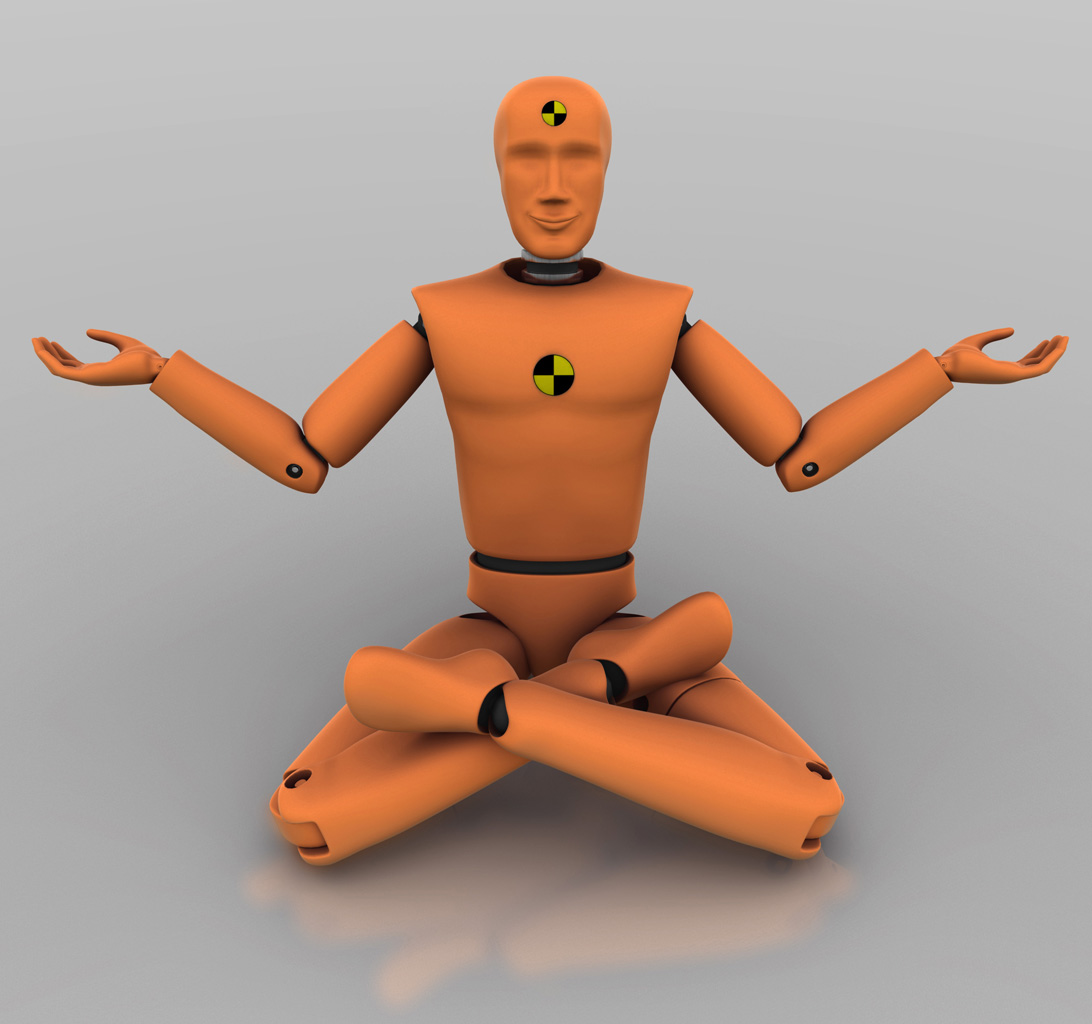
\includegraphics[width=0.7\textwidth]{Enddokumentation/Titelbild.JPG}
%        \end{figure*}
        
        \vfill{}
        {\normalsize Hochschule Luzern - Technik \& Architektur\\
         PREN 1}\\[0.6cm]
        {\normalsize Horw, Hochschule Luzern - T\&A, \today}
    \end{center}
\end{titlepage}

    \begin{titlepage}
    \begin{center}
        \parindent0pt{\Huge\bfseries \myDokumentTyp}\\[0.5cm]
		{\huge PREN 2, Team 32}\\[2em]
        \begin{tabular}{ll}
            Yves Studer                & Thomas Wiss \\
            Dorfstrasse 28             & Bachhüsliweg 4a \\
            6264 Pfaffnau              & 6042 Dietwil \\
            +41 79 705 48 88           & +41 79 604 93 61 \\
            yves.studer@stud.hslu.ch   & thomas.wiss@stud.hslu.ch \\
                                       & \\
            Livio Kunz                 & Niklaus Manser \\
            Hubelmatt 7                & Brunnmattstrasse 11\\
            6206 Neuenkirch            & 6010 Kriens \\
            +41 79 811 53 03           & +41 77 405 58 56 \\
            livio.kunz@stud.hslu.ch    & niklaus.manser@stud.hslu.ch \\
                                       & \\
            Matteo Trachsel			   & Roger Gisler \\
            Ogimatte 7                 & Eyrüti 16\\
            3713 Reichenbach           & 6467 Schattdorf\\
            +41 79 511 57 88           & +41 79 729 55 34 \\
            matteo.trachsel@stud.hslu.ch & roger.gisler@stud.hslu.ch \\
            						   & \\
            Pascal Roth			       & \\
            Dorfstrasse 18			   & \\
            6275 Ballwil		       & \\
            +41 79 717 68 94	       & \\
            pascal.roth@stud.hslu.ch   & \\
        \end{tabular}\\
        \vspace{3em}
        {\Huge \myTitel}\\[5em]
        Dozent: Markus Thalmann\\[2em]
        Hochschule Luzern - Technik \& Architektur\\   
        Interdisziplinäre Projektarbeit 2015
        \vfill{}
        Horw, Hochschule Luzern - T\&A, \today
    \end{center}
\end{titlepage}
    %
    % Inhlatsverzeichnis umbenennen und anschliessend einen Seitenumbruch
    %  
    
\section*{Abstract}
In der nachfolgenden Dokumentation wird der Prozess der Konzeptfindung für die Herstellung eines
autonomen Ballwerfers beschrieben. Durch die Aufteilung der Aufgabenstellung in Problembereiche werden
mehrere unterschiedliche Konzepte geschaffen. Von den erstellten Konzepten wurde eines weiter zu einem
Feinkonzept ausgearbeitet, in welchem sämtliche verwendeten Komponenten spezifiziert werden. Als
erstes wird das Startsignal von einem Laptop drahtlos via Bluetooth übertragen. Daraufhin lokalisiert
der fixstehende Ballwerfer den Korb unter Verwendung einer Smartphonekamera, auf welchem eine
entsprechende Applikation zur Korberkennung läuft. Ist die Position einmal bestimmt, wird die Position
an den Controller weitergegeben, welcher den Steppermotor für die Ausrichtung des Werfers betätigt und
anschliessend die Ballzuführung startet. Der Ballwerfer selbst ist statisch und richtet sich an der
Startposition für einen gewinkelten Wurf aus. Einmal ausgerichtet, werden die Bälle einzeln unter
Verwendung von Schwungrädern geworfen.

 
    \renewcommand{\contentsname}{Inhalt}
    \tableofcontents
    \newpage 
    %
    % Start mit der eigentlicher Arbeit
    %    
    \section{Danksagung}
Das PREN Team 32 wurde während der ganzen Projektphase von verschiedenen Dozenten der Hochschule Luzern Technik \& Architektur unterstützt. 
Ein grosses Dankeschön geht an Herr Markus Thalmann, Herr Ernst Lüthi und Herr Martin Vogel. Sie haben das Team aktiv unterstützt, 
indem sie wertvolle Hinweise und Ratschläge zum Produkt gegeben haben.

    \section{Einleitung}
Im heutigen Arbeitsumfeld ist es unerlässlich, dass man in der Lage ist, in 
einem interdisziplinär zusammengesetzten Team zu arbeiten. An diesem Punkt 
setzt die Hochschule Luzern Technik \& Architektur mit dem Modul 
\enquote{Produktentwicklung} (PREN) an. Das Ziel dieses Moduls ist, anhand 
einer Aufgabenstellung einen Entwicklungsprozess zu durchlaufen, in einem 
Team eine geeignete Lösung zu eruieren und umzusetzen. Die Teams bestehen 
aus Studierenden aus den Studiengängen Elektrotechnik, Informatik und 
Maschinenbau. Dieses Modul ist in zwei Teile aufgeteilt und erstreckt sich 
über zwei Semester. In PREN 1 wird anhand der Aufgabenstellung ein Konzept 
entwickelt, welches im anschliessenden Semester, in PREN 2, umgesetzt wird.\\
\\
In diesem Rahmen erhielten die Teams dieses Jahr die Aufgabe, einen autonomen 
Ballwerfer zu erarbeiten. Das Ziel besteht darin, fünf Tennisbälle in möglichst 
kurzer Zeit in einen Korb zu befördern. Als weiteres Bewertungskriterium gilt 
das Gewicht des Produkts, welches ab zwei Kilogramm einen stufenweisen 
Punkteabzug zur Folge hat. Das Spielfeld ist sowohl seitlich, als auch in der 
Höhe begrenzt. Zusätzlich befindet sich am hinteren Ende eine vertikale Wand, 
vor welcher der Korb auf einer zu dieser Rückwand parallelen Linie platziert 
wird. Die endgültige Position des Korbes wird kurz vor der Abgabe des Startsignals 
durch einen Dozenten festgelegt und ist somit zu Beginn nicht bekannt. Die 
Übermittlung des Startsignals muss drahtlos erfolgen, nach Ausführen der Aufgabe, 
muss entweder ein akustisches oder ein optisches Endsignal ausgegeben werden.\\
\\
In PREN 2 wurde nun das Konzept, welches im ersten Teil von PREN erarbeitet wurde, 
umgesetzt. Das bedeutet, dass ein lauffähiges Funktionsmuster gebaut wurde. 
Ausgehend von den gewonnenen Erkenntnissen des ersten Modulteils, konnten die 
einzelnen Bestandteile gebaut oder umgesetzt werden. In diversen Testläufen 
wurden Systemparameter eruiert und angepasst. Alle Komponenten des 
Gesamtfunktionsmusters wurden aufeinander angepasst und der Ballwerfer konnte in 
Betrieb genommen werden. 
    \newpage
    \section{Von der Idee zum Produkt}
Die Idee der Ballmaschine wurde im Modul PREN 1 ausführlich evaluiert und geplant. 
Ein sehr ausgereiftes Konzept wurde aufgestellt und es blieben nur noch wenige 
technische Unklarheiten. Mit dem Ziel, das erarbeitete Konzept aus PREN 1 möglichst 
unverändert in die Realität umzusetzen, startete das Modul PREN 2.
Bis zum Schluss wurde das Grundkonzept beibehalten und nur wenige kleine Anpassungen 
vorgenommen. So mussten z.B einige Kerben an der Acrylglaskonstruktion verstärkt werden
oder die Verzahnung der Grundplatte um einen grösseren Schwenkwinkel erweitert werden. 
Somit konnte gezeigt werden, dass das erarbeitete Konzept in die Praxis umgesetzt 
werden kann. Weiter stehen die Ziele, welche vom Team in PREN 1 in der folgenden Reihenfolge definiert 
worden sind, im Vordergrund,
\begin{enumerate}
	\item Treffgenauigkeit
	\item Geschwindigkeit
	\item Gewicht
\end{enumerate}
    \section{Grundaufbau}
	Im kommenden Kapitel wird der Grundaufbau des kompletten Ballwerfers ausführlich erläutert. 
	In diesem Sinne wird auf sämtliche Hard- und Software-Komponenten eingegangen.
    Der Ballwerfer ist so konzipiert, das er aus einem fix stehenden Basismodul besteht, 
    welches in der Mitte des Startbereiches positioniert wird. Die Abwurfeinheit, welche 
    den Ballwurfmechanismus und die Ballzuführung beinhaltet, ist auf dem Basismodul 
    drehend gelagert. Weiter ist auch das Smartphone für die Korberkennung und alle 
    Steuereinheiten auf dem Basismodul angebracht. Das Startsignal wird mittels WLAN 
    von einem externen Notebook übertragen. Im folgenden Bild sieht man die komplette Ballmaschine mit den Hauptkomponenten, Förderband
    Ausrichteinheit mit Brushlessmotor, Beschleunigungsräder und den Netzteilen, siehe Abbildung \ref{abb:Ballmaschine}.
    \begin{figure}[h!]
    	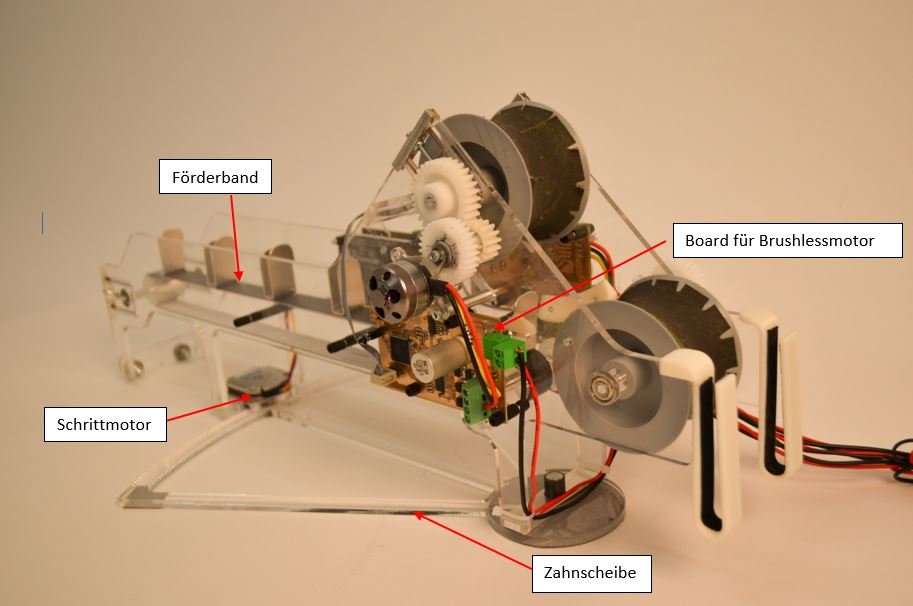
\includegraphics[width=.93\textwidth,clip,trim=0mm 0mm 0mm 0mm]
    	{Enddokumentation/Bilder/Geraeteuebersicht_2.jpg}
    	\centering
    	\caption{Aufsicht auf die rechte Seite}
    	\label{abb:Ballmaschine}
    \end{figure}
    
    Der ganze Aufbau des Ballwurfmechanismus ist möglichst simpel gehalten. Er besteht 
    hauptsächlich aus zwei $5\si{\milli\meter}$ dicken Acrylglasplatten, in welcher alle mechanischen 
    Vorrichtungen gelagert sind. Durch diesen Aufbau können Änderungen schnell und 
    einfach angepasst werden. Die Ausrichtung des Abwurfmechanismus erfolgt durch 
    einen flachen Steppermotor, welcher in der drehenden Abwurfeinheit angebracht 
    ist. Dadurch wird die Bauhöhe des Ballwerfers tief gehalten, was einen grossen 
    Vorteil in Sachen Stabilität bietet. Die Drehachse der Abwurfeinheit ist an der Spitze des 
    Ballwerfers mit einem Bolzen angebracht. Somit bleibt die Abwurfposition der 
    Tennisbälle konstant am gleichen Ort. Die Bälle werden durch zwei 
    Beschleunigungsräder beschleunigt, welche jeweils einzeln 
    über eine Übersetzung mit einem Brushlessmotor auf Touren gebracht. Die Beschleunigungsräder 
    drehen gegenläufig, wobei die Tennisbälle zum Abwurf dazwischen hindurchgeführt werden. Die Zuführung zu den Beschleunigungsräder erfolgt mit 
    einem Förderband. Das Förderband transportiert die Bälle mit einer 
    konstanter Geschwindigkeit zu den Beschleunigungsräder, damit alle Tennisbälle die 
    gleiche Startenergie aufweisen. Dadurch ist eine gleichmässige Wurfweite und eine 
    hohe Reproduzierbarkeit gewährleistet. \\
    Die zwei nachkommenden Bilder zeigen einer Übersicht der verschiedenen weiteren Komponenten, welche im Verlauf der Dokumentation explizit erklärt werden, siehe Abbildungen \ref{abb:Aufsicht auf die linke Seite} und \ref{abb:Frontale Aufsicht}.
	
	\begin{figure}[h!]
	   	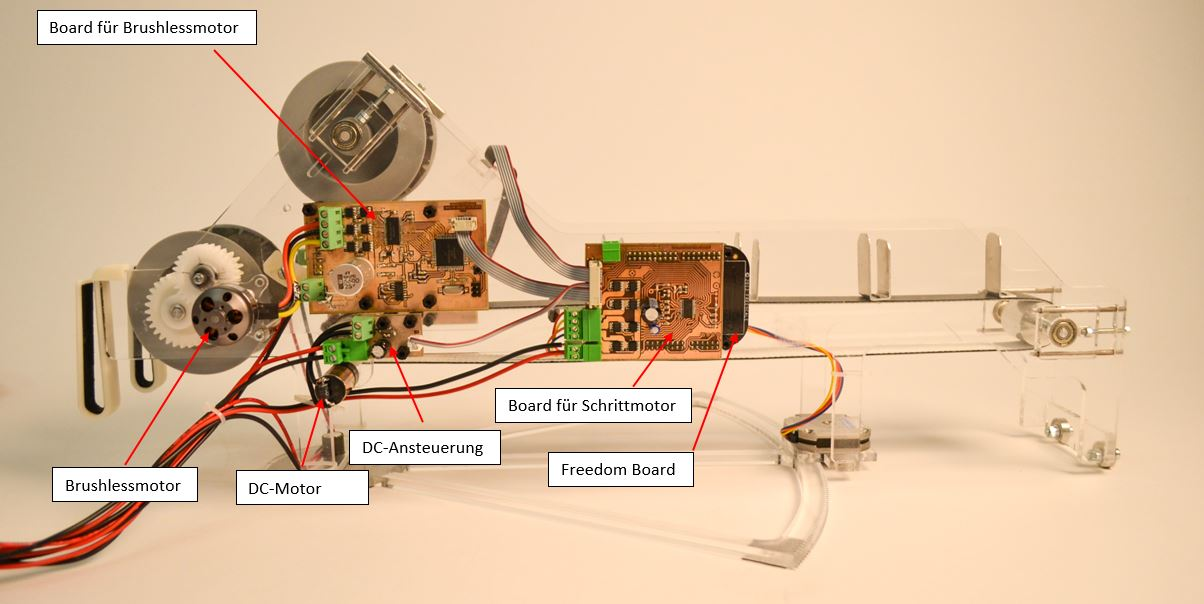
\includegraphics[width=.93\textwidth,clip,trim=0mm 0mm 0mm 0mm]
	   	{Enddokumentation/Bilder/Geraeteuebersicht_1.jpg}
	   	\centering
	   	\caption{Aufsicht auf die linke Seite}
	   	\label{abb:Aufsicht auf die linke Seite}
	\end{figure}
	
	\begin{figure}[h!]
	   	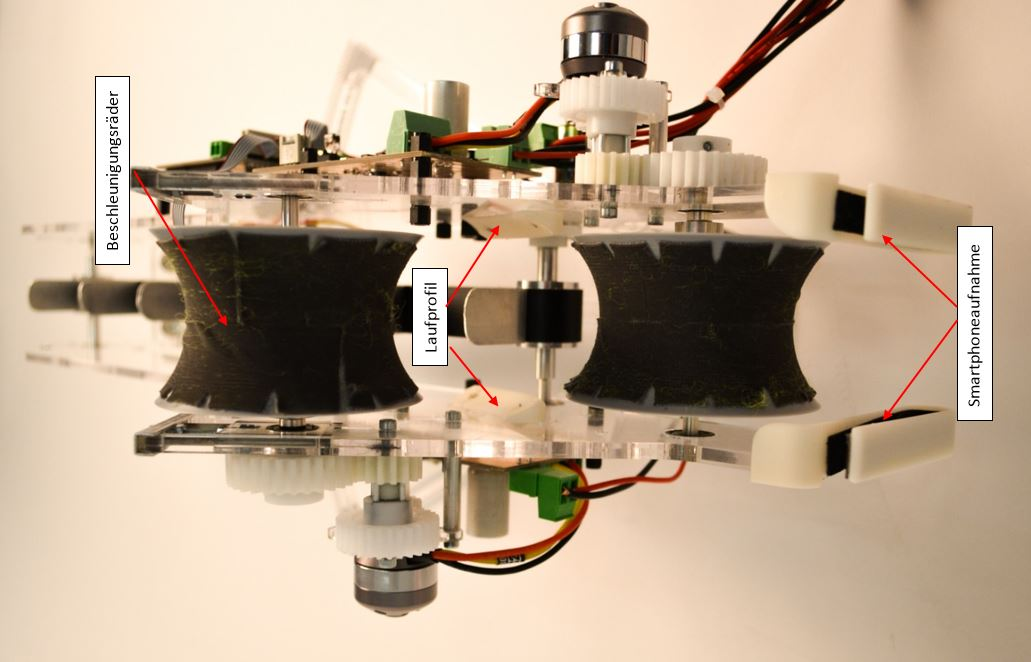
\includegraphics[width=0.58\textwidth,clip,trim=0mm 0mm 0mm 0mm]
	   	{Enddokumentation/Bilder/Geraeteuebersicht_3.jpg}
	   	\centering
	   	\caption{Frontale Aufsicht}
	   	\label{abb:Frontale Aufsicht}
	\end{figure}
    
    
    \newpage
    \subsection{Herstellung Acrylglas}
		Für die Seitenwände, die Zahnscheibe und für die Verbindungsstege wurde eine 
		$5\si{\milli\meter}$ Dicke Acrylglas (PMMA) Platte verwendet. Die Konturen 
		wurden mit dem Laser an der HSLU gefertigt. Damit der Laser die Daten lesen 
		konnte, wurde aus der CAD-Datei des Seitenprofiles eine dxf-Datei erstellt. Um die Nachbearbeitung 
		möglichst gering zu halten, wurden auch die Lager- und Durchgangsbohrungen 
		für die Schrauben direkt auf das Fertigmass gelasert. Die Lager passten dabei 
		sehr genau in die Bohrungen, sodass sie ein wenig klemmten und trotzdem keine 
		starken Spannungen erzeugten, die allenfalls zu Rissen führen könnten. Dies 
		wurde im Vorfeld getestet (siehe Doku PREN 1). Die einzigen Nachbearbeitungen 
		waren die Bohrungen an den Seitenwänden und an den Spannelementen. 
		Dabei musste auf eine gute Kühlung geachtet werden, da die Restwandstärke nur 
		noch je $1\si{\milli\meter}$ beträgt und das Acrylglas schnell weich wird. 
		Ebenfalls musste die Schnittgeschwindigkeit für das Bohren drastisch gesenkt 
		werden gegenüber einem normalen Kunststoff wie PE. Die Bohrungen an 
		den Seitenwänden wurden auf einer Universalfräsmaschine durchgeführt, die über eine 
		horizontale Frässpindel verfügt (siehe Abbildungen \ref{fig:Acrylglas_1} und 
		\ref{fig:Acrylglas_2}). Die Bohrungen für die 
		Elekronikprints und andere kleine Anpassungen wurden ebenfalls erst nach dem 
		Lasern gefertigt. Zum Beispiel die Ansenkungen für die Schraubenköpfe oder bei 
		den Elekronikprints weil der endgültige Platz noch nicht festgelegt war.
		\begin{figure}[h!]
			\begin{minipage}[hbt]{0.5\textwidth}
		   		\centering
		   		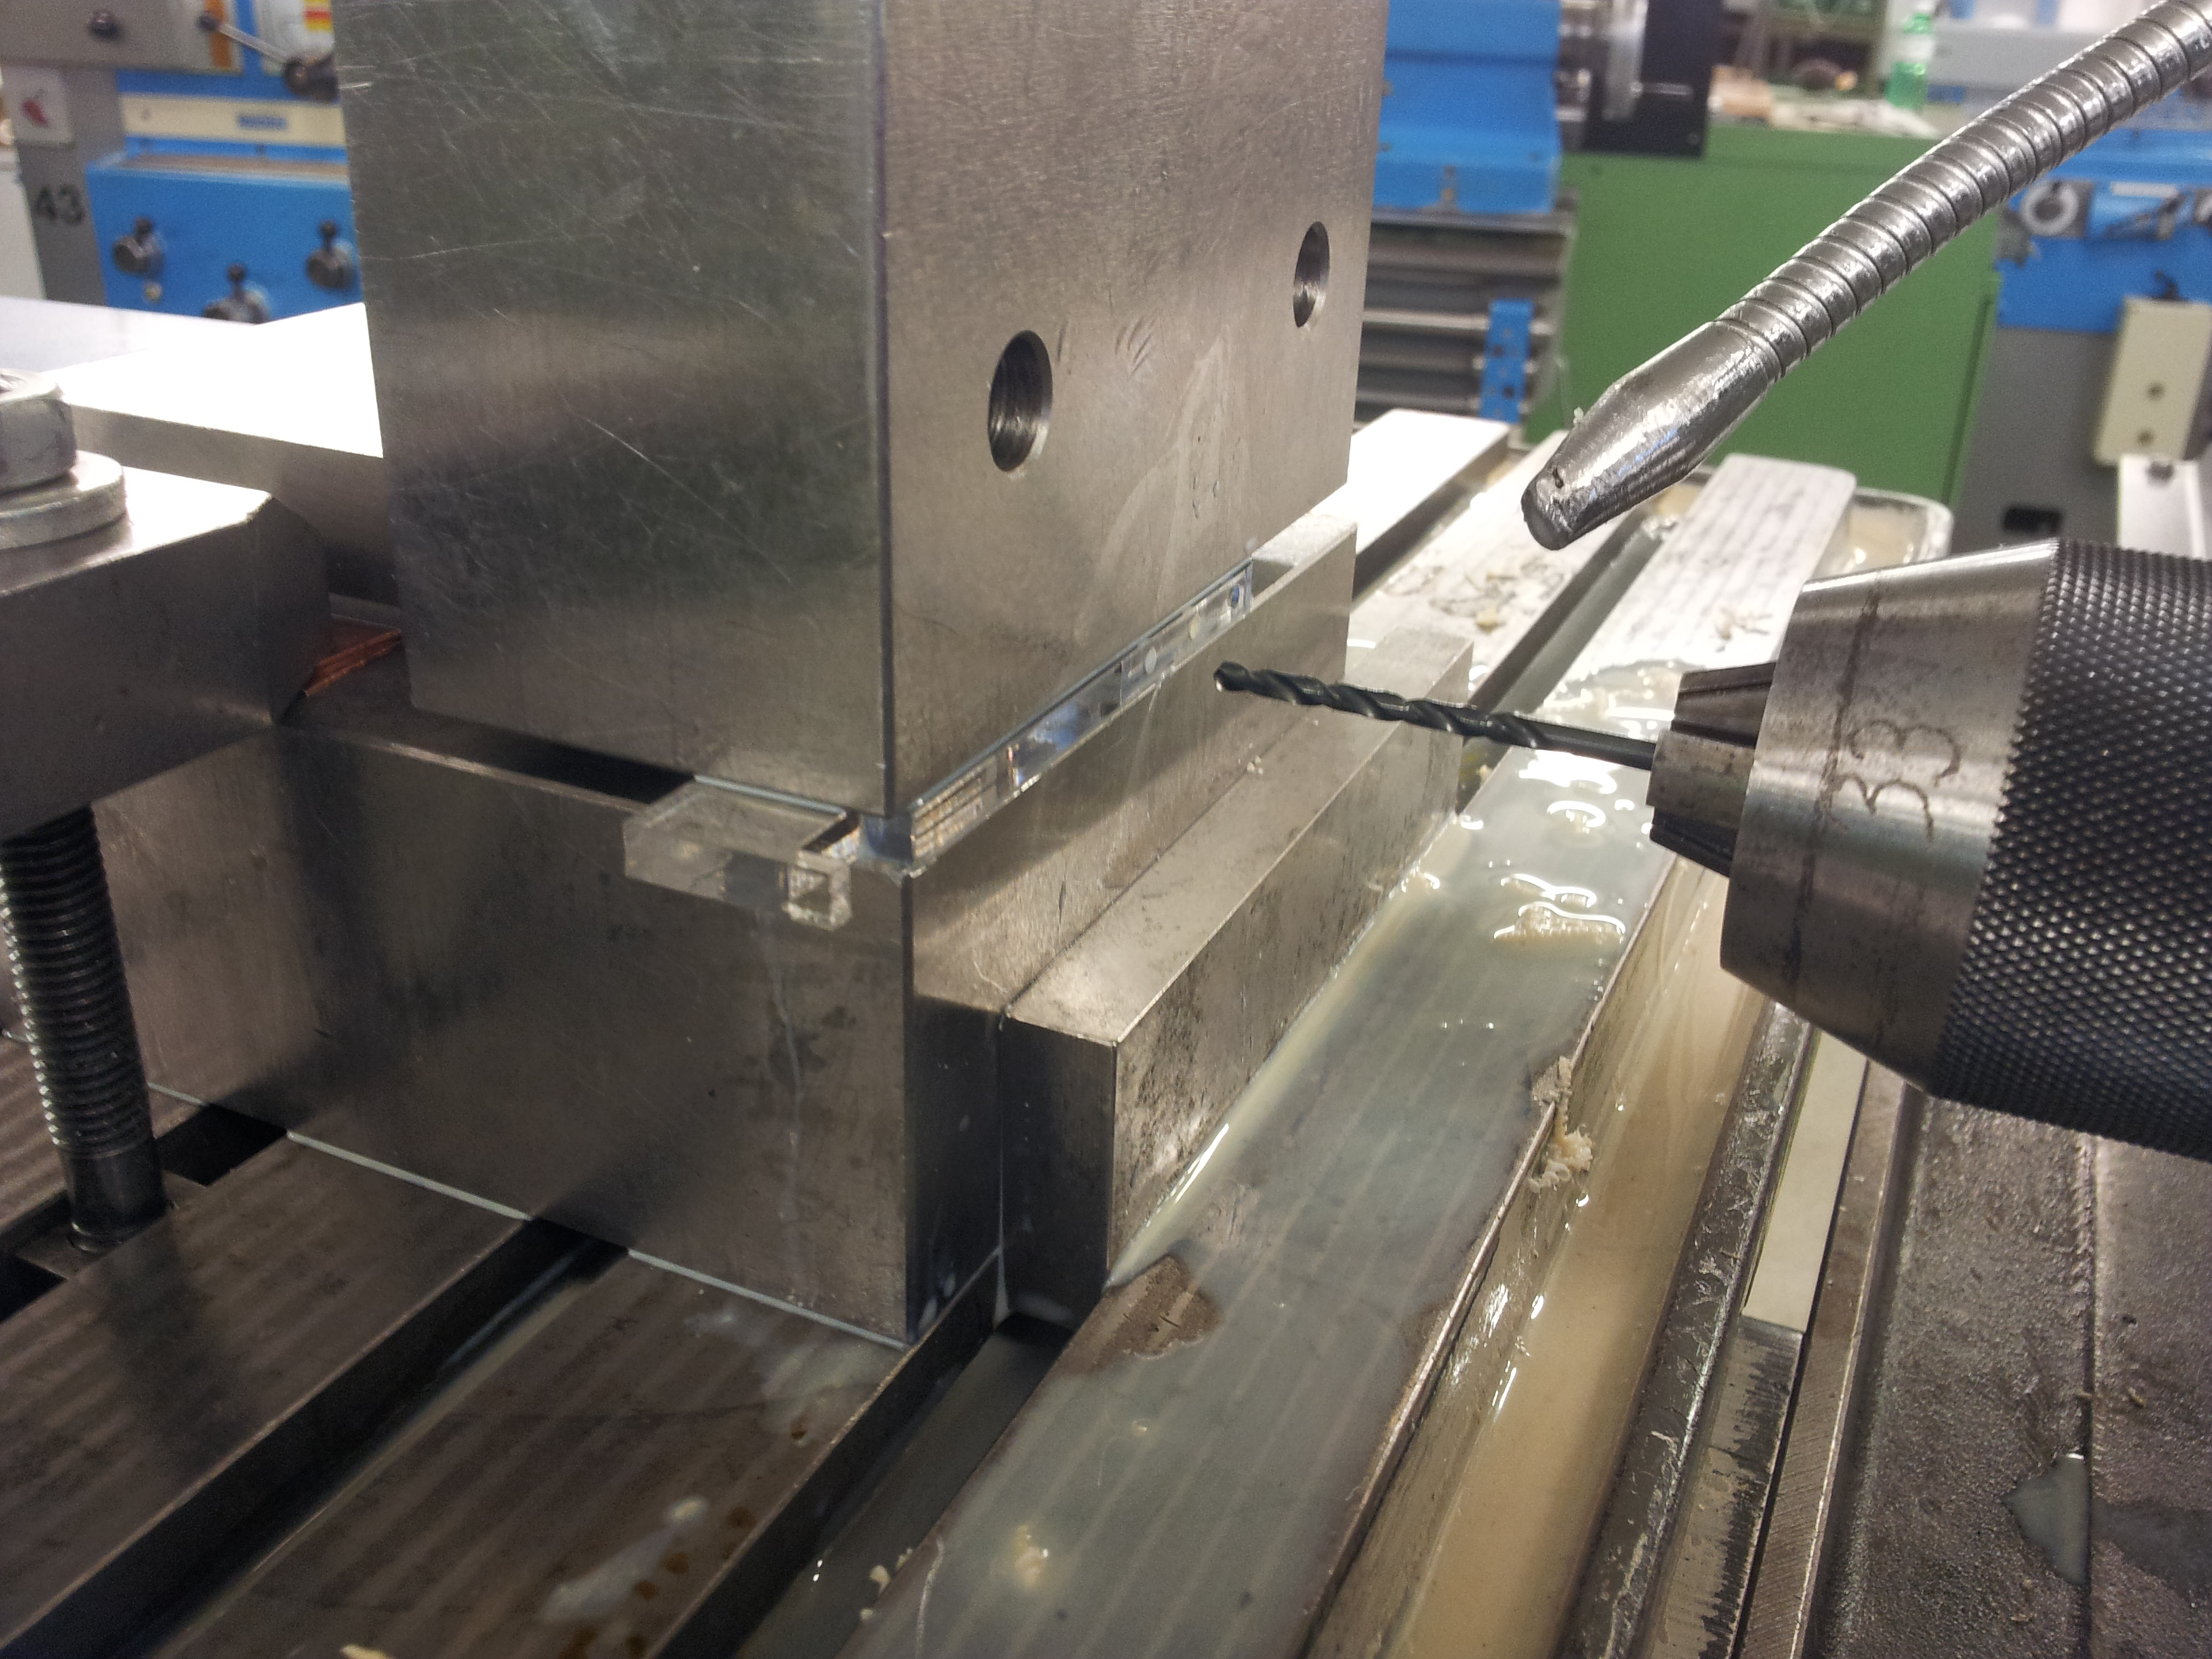
\includegraphics[width=1\textwidth,clip,trim= 0mm 0mm 0mm 0mm]
		   		{Enddokumentation/Bilder/Herstellung_Acrylglas_1.jpg} 
		   		\caption{Herstellung der Acrylglas-Teile}
		   		\label{fig:Acrylglas_1}
			\end{minipage}
			\hfill
			\begin{minipage}[hbt]{0.5\textwidth}
		   		\centering
		   		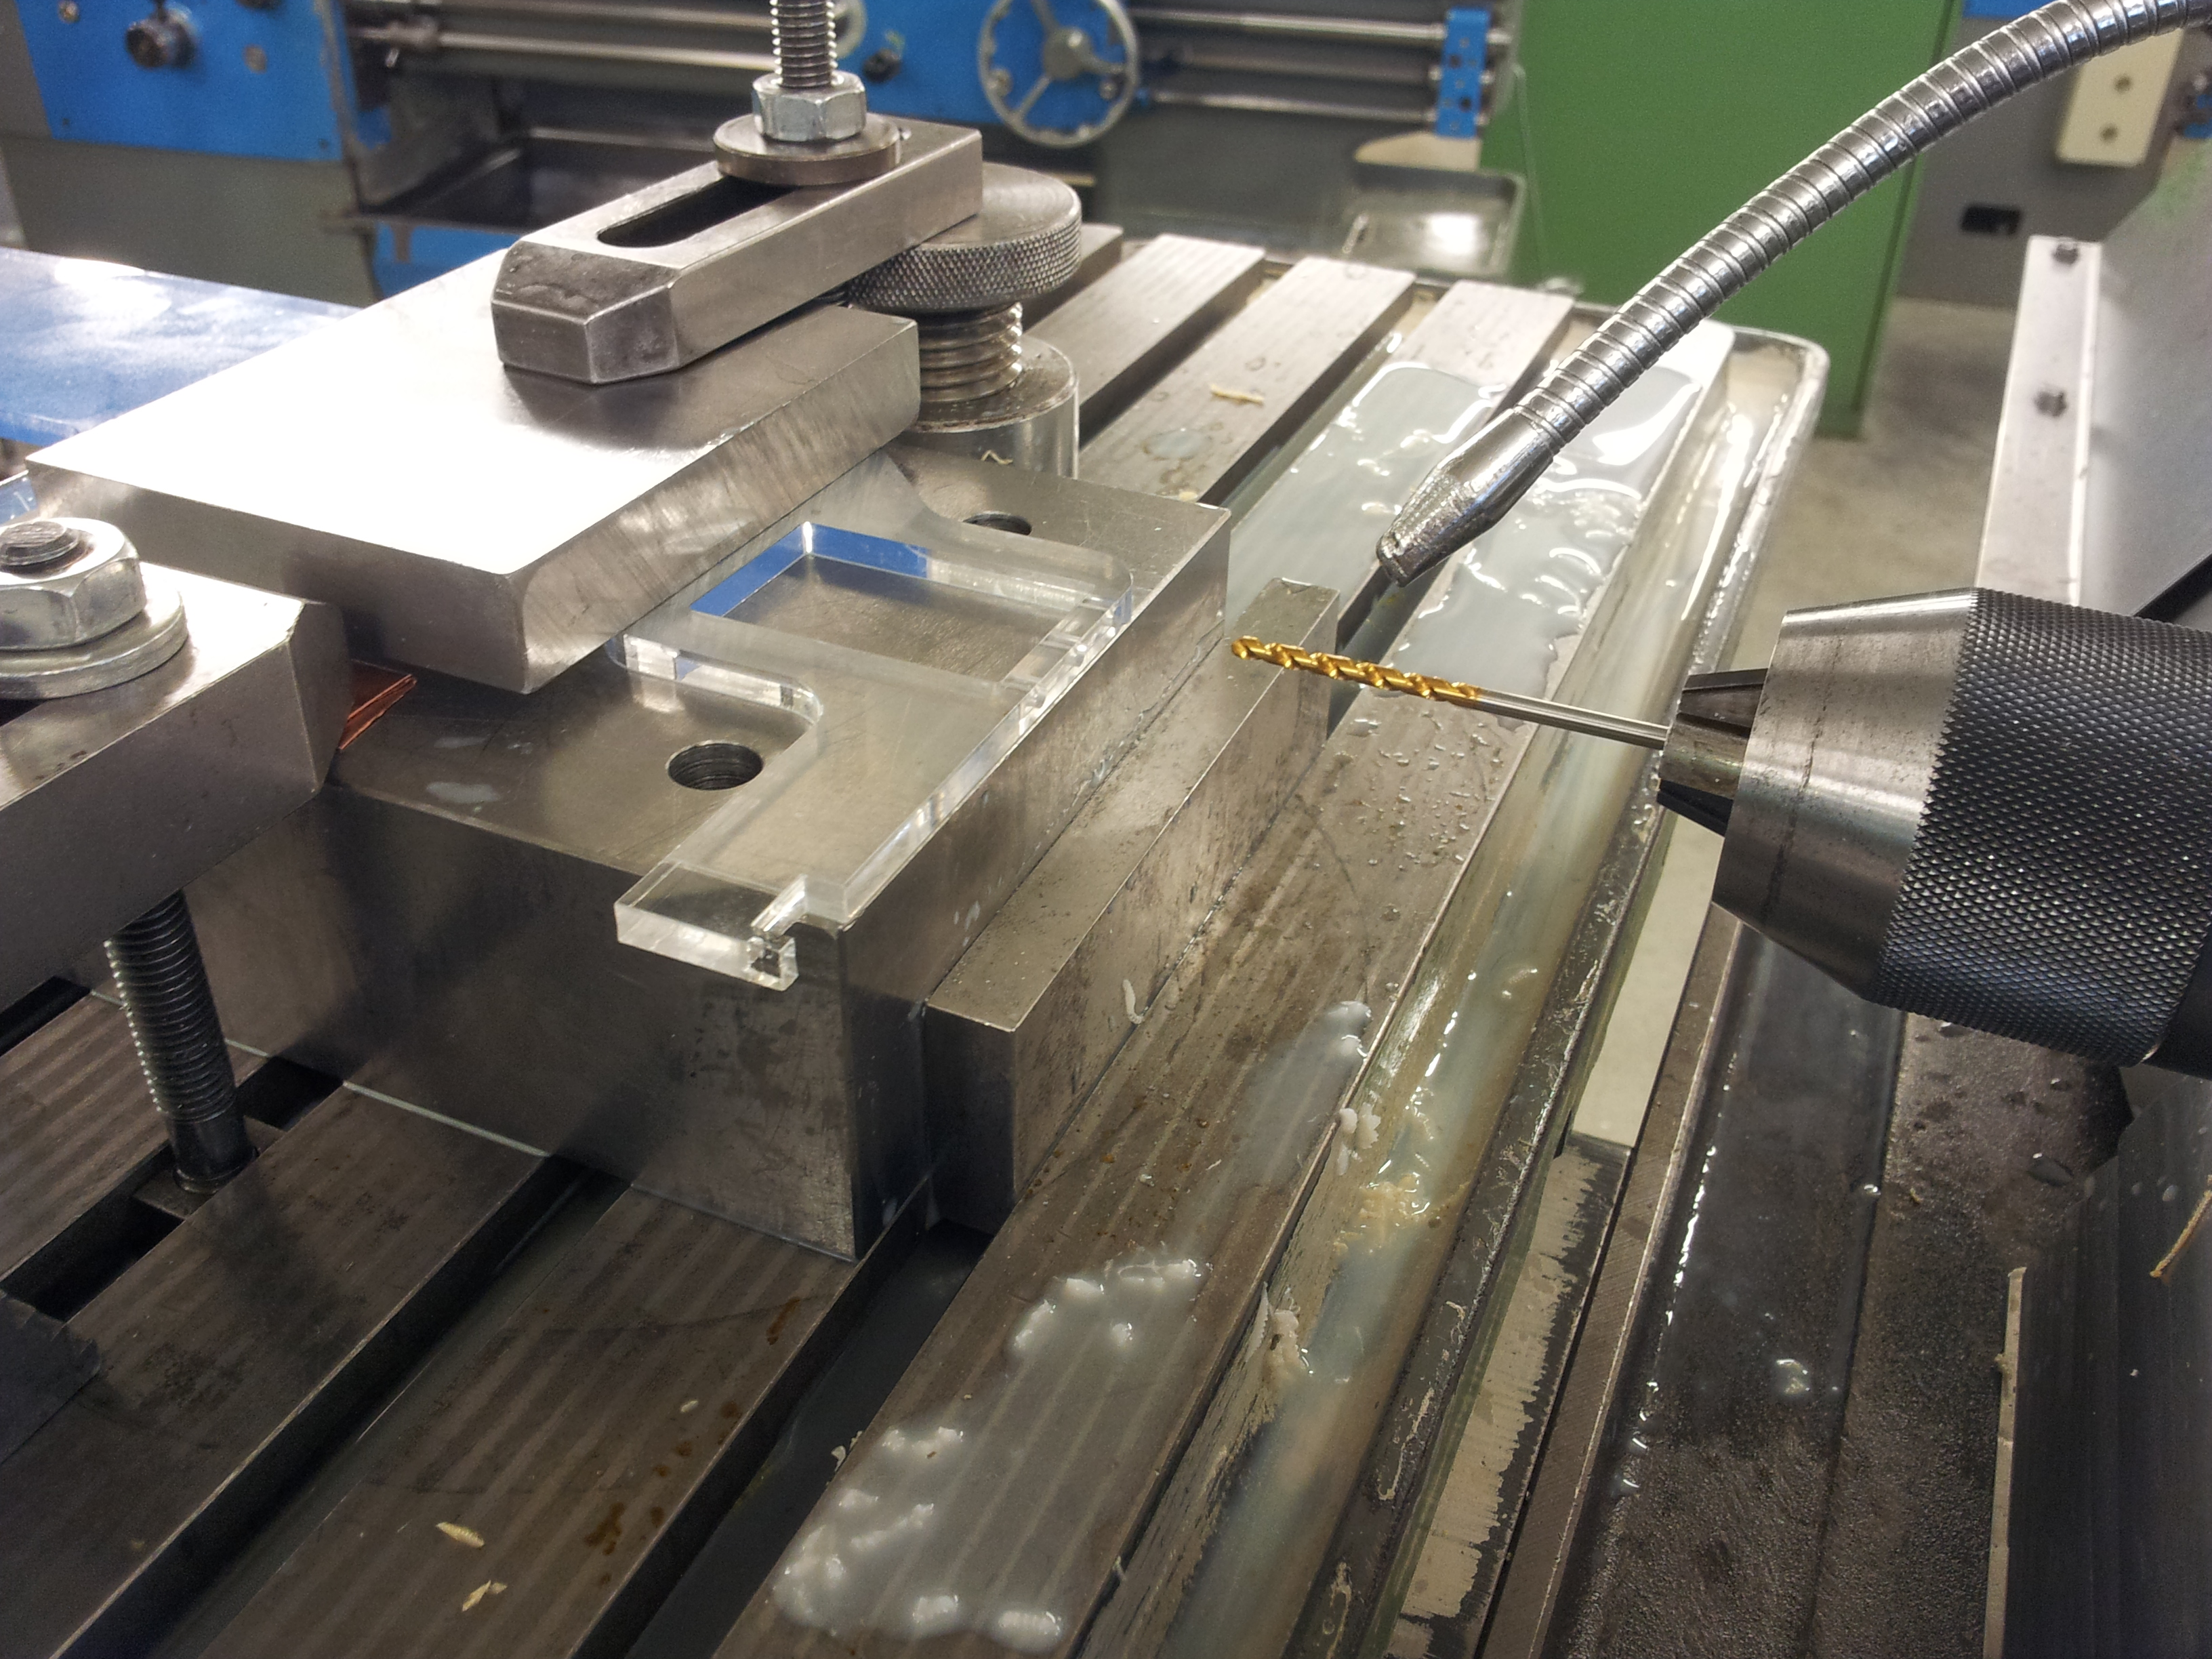
\includegraphics[width=1\textwidth,clip,trim= 0mm 0mm 0mm 0mm]
		   		{Enddokumentation/Bilder/Herstellung_Acrylglas_2.jpg} 
		   		\caption{Herstellung der Acrylglas-Teile}
		   		\label{fig:Acrylglas_2}
			\end{minipage}
		\end{figure}
		
		Neben den mechanischen Hauptkomponenten gibt es auch in der Elektronik sogenannte Grundelemente. 
		
    \subsection{Hauptcontroller}
    	
        Die gesamte Hardware wird über das Freedom-Board\footnote{Development-Board vom 
        Hersteller Freescale, Typ FRDM-KL25Z} gesteuert. Dieses Board hat einen internen UART\footnote{\textbf{U}niversal \textbf{A}synchronous \textbf{R}eceiver 
        \textbf{T}ransmitter, eine serielle Schnittstelle} to USB Converter, über diesen 
        das Smartphone mit dem Freedom-Board kommuniziert. Die Software des Boards besteht aus einem 
        Betriebssystem, dessen Haupttask kontinuierlich den UART Eingangspuffer abruft 
        und die angekommenen Befehle ausführt. Ein wichtiger, nur einmal gebrauchter Task, 
        ist die Initialisierung des Stepperboards, siehe Anhang Kapitel \ref{sec:StepperAnsteuerung}. Der Controller 
        verfügt über zwei SPI\footnote{Serial Peripheral Interface, ein synchroner serieller Datenbus }-Schnittstellen. An einer ist das besagte Stepperboard und 
        an der anderen die beiden Brushless-Boards angeschlossen. Weiter wird ein PWM\footnote{pulse width modulation}-Port 
        verwendet, um den Motor der Ballnachführung anzutreiben, siehe Kapitel 
        \ref{sec:Foerderband}.  

   
    \subsection{Spannungsversorgung}       
        \begin{wrapfigure}{r}{0.35\textwidth}
           	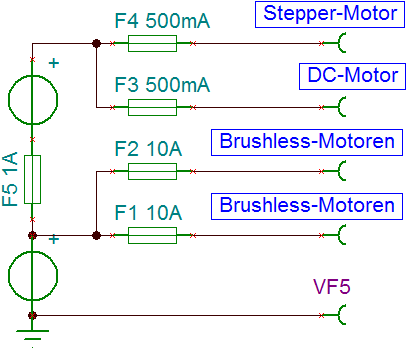
\includegraphics[width=0.35\textwidth,clip,trim=0mm 0.5mm 0mm 0mm]
           	{Enddokumentation/Bilder/BeschaltungNetzteile.png}
           	\centering
           	\caption{Schema der Spannungsversorgung} 
           	\label{abb:Spannungsversorgung}
        \end{wrapfigure}
        Gemäss Datenblatt sind die verwendeten Brushless-Motoren mit einer Versorgungsspannung 
        von $12\si{\volt}$ bei einem maximalen Strom von $11\si{\ampere}$ spezifiziert. 
        Der Steppermotor und der DC-Motor sind gemäss Datenblatt für das Betriebsspannung FreeRTOS 
        von $24\si{\volt}$ ausgelegt. Die Spannungsversorgung wird mit zwei Server-Netzteilen 
        realisiert, die je $12\si{\volt}$ mit maximal $60\si{\ampere}$ liefern. Aus 
        Sicherheitsgründen wird für jeden Motor eine separate Sicherung verwendet. Das Schema 
        in Abbildung \ref{abb:Spannungsversorgung} zeigt, wie die Spannungsversorgung 
        umgesetzt ist. Das Freedom-Board wird über USB vom Akkumulator des Smartphone 
        gespeist. Sämtliche Datenblätter zu den verwendeten Motoren sind im Anhangsdokument 
        angefügt. Das zweite Netzteil wurde so umgebaut, dass es potentialfrei arbeitet. So 
        ist es möglich, dass es die $12\si{\volt}$ auf die Spannung des ersten Netzteils 
        generieren kann. Die Sicherung zwischen den beiden Netzteilen ist als Sicherheit 
        hinzugefügt für den Fall, dass es Probleme mit der Potentialfreiheit gibt.	
        
        \subsection{Smartphone auf dem Ballwerfer}
        Das eingesetzte Smartphone ist ein Samsung Galaxy Nexus I9250. Es führt diverse Aufgaben aus. Dazu zählt 
        die Bildaufnahme, die Auswertung des Bildes, die Berechnung des Winkels, die Kommunikation 
        mit dem Desktop-Computer (Startgerät) und mit dem Freedom-Board.
    \clearpage
    \section{Softwarearchitektur}
    \subsection{Vom Winkel zum Board}

\begin{figure}[h!]
	\includegraphics[width=0.5\textwidth,clip,trim=20mm 120mm 100mm 40mm]  % trim=l b r t
	{Enddokumentation/Bilder/UebersichtWinkelberechnung.pdf}
	\centering
	\caption{Übersichtsskizze zur Winkelberechnung}
	\label{abb:UebersichtWinkelberechnung}
\end{figure}

Wie in Abbildung \ref{abb:editedPicture} ersichtlich ist, erstellt der Detektor ein Schwarz/Weiss Bild, welches den oberen Rand des Korbs zeigt. 
Um das Gerät auf den Korb auszurichten, muss der Winkel (siehe a in Abbildung \ref{abb:UebersichtWinkelberechnung}) errechnet werden, 
damit man den Winkel anschliessend in die Anzahl MircoSteps des Schrittmotors umrechnen kann.
\newline
\newline
Aus diesem Bild wird nun mittels Trigonometrie der Winkel berechnet. 
Dazu wird zuerst die Länge Gegenkathete (siehe G in Abbildung \ref{abb:UebersichtWinkelberechnung}) 
aus dem Schwarz/Weiss Bild errechnet. Ausgehend vom der Mitte des Spielfelds kann die Distanz zum Mittelpunkt des 
Korbs bestimmt werden. Diese Länge liegt zuerst als Anzahl Pixel vor, 
kann anschliessend mit einem (variablen) Umrechnungsverhältnis Pixel zu Zentimeter in Zentimeter umgerechnet werden.
Die Ankathete (siehe A in Abbildung \ref{abb:UebersichtWinkelberechnung}) ist durch das Spielfeld auf die Länge von 170 cm fixiert.
Mit diesen beiden Werten lässt sich nun mit dem Arkustangens der resultierende Winkel errechnen.
Dieser Winkel kann mit dem Umrechnungsverhältnis (siehe Kapitel \ref{sec:Aufloesung}) von Microsteps zu Grad 
in die Anzahl Schritte für den Schrittmotor umgewandelt werden. Um die Drehrichtung des Schrittmotors festzulegen, besteht der 
Befehl des Schrittmotors aus einer Drehrichtung und der Anzahl Schritte. Hat der Winkel einen positiven Wert, muss der Anzahl 
Schritte für den Schrittmotor ein  \enquote{r} für die Drehrichtung vorangestellt werden, ist der Winkel negativ, ein  \enquote{f} 
(siehe Abbildung \ref{abb:UebersichtWinkelberechnung}).  
\newline
\newline
\textit{Nähere Angaben zum Schrittmotor und dessen Ansteuerung sind im Anhang unter der Dokumentation des Steppers der ET-Gruppe verfügbar.}
\newline
\newline
Sollte als Beispiel der errechnete Winkel $-7,8\si{\degree}$ sein, würde das Freedom-Board vom Android-Phone folgenden 
Befehl erhalten: f 15320 (Umrechnungsverhältnis: $1\si{\degree}$ entspricht 1964 Microsteps).
Da die Hypotenuse mit der Länge der Gegenkathete und damit auch mit grösserem Winkel ?? linear, exponentiell,.. ?? an Länge zunimmt, 
hat dies auch eine Verlängerung der Wurfdistanz zur Folge. Um diesem Umstand Rechnung zu tragen, muss die Drehzahl des 
Brushless-DC-Motors entsprechend dem Winkel angepasst werden. Weil das Gerät symmetrisch in der Mitte des Spielfelds platziert ist, 
kann das Vorzeichen des Winkels ausser Acht gelassen werden, denn auf beide Seiten nimmt die Distanz im selben Masse zu.
Dazu wird die folgende Formel verwendet (Die gilt nur bei linearem Anstieg):
\newline
\newline
Formel (muss noch verifiziert werden)
 
\begin{equation}
RPM = RPM_{min} +  \left( \frac{RPM_{max} -RPM_{min}}{Winkel_{max}} \cdot |\text{berechneter Winkel}| \right)
\end{equation}
 
Um den Zeitverlust möglichst klein zu halten, wird die neu errechnete Umdrehungszahl sofort nach erhalten des Winkels an das 
Freedom-Board gesendet, damit die Motoren auf die neue Drehzahl beschleunigt werden können.
Nachdem das Gerät ausgerichtet ist und die Brushless-DC-Motoren die neu errechnete Drehzahl erreicht haben, kann das Förderband 
für die Ballzuführung eingeschaltet werden. Dies erfolgt mit einem simplen Befehl \enquote{DC setpwm <Wert>}. 
Um alle Motoren, welche noch in Betrieb sind, abzuschalten, muss noch eine Serie von Shutdown-Befehlen an das 
Freedom-Board gesendet werden. 


            
            

    % Noch Titel für folgende Komponenten setzten
    \subsection{USB Connection}
Um verschiedene Befehle und den vom Detektor berechneten Winkel vom Android-Phone an das Freedom-Board (KL25Z) 
zu senden, wird eine USB\footnote{Universal Serial Bus}-Schnittstelle zwischen diesen zwei Geräte verwendet.
Da Android keine native Anbindung an MicroController-Boards via USB zur Verfügung stellt, muss auf 
Frameworks von Drittanbietern zugegriffen werden. In unserem Fall verwenden wir UsbSerial \cite{Inf:UsbSerial} als support-library. 
Wie im Namen ersichtlich, 
handelt es sich dabei um eine virtuelle serielle Schnittstelle (COM-Schnittstelle\footnote{Component Object Model})
für den USB-Port eines Android-Gerätes. Dieser Serial Controller erlaubt es programmatisch alle nötigen Konfigurationen 
(Baudrate, Databit, Stopbits, Paritybit, Flowcontrol) für das Board zu setzen. Mittels einer einzigen 
Methode können nun anschliessend Bytes gesendet werden. Um ein ressourcenfressendes Pollen am Eingang zu vermeiden, 
bietet die Library eine Callback-Funktion, die aufgerufen wird, wenn Daten am Eingang eintreffen.
Mit dem Programmieren und Erstellen eines ersten Prototyps (Android App, siehe Abbildung \ref{abb:ScreenshotSerialPortExample}) musste die Frage geklärt werden, 
ob mit der support-library das Senden eines einzelnen Strings (Char) zum Freedom-Board und das Echo des 
Boards auf dem Bildschirm des Smartphones ausgegeben werden kann. Nach einem Testlauf zeigte sich, dass
das Senden des Chars soweit nachvollziehbar einwandfrei funktioniert. Beim Empfangen der Daten zeigte 
sich, dass beim parsen der Bytes im Code der support-library ein oder zwei Bits falsch gesetzt wurden. 
Das hatte zur Folge, dass gewisse Buchstaben oder Zahlen nicht mehr korrekt in ASCII\footnote{American 
Standard Code for Information Interchange} respektive UTF-8\footnote{Universal Coded Character Set + 
Transformation Format—8-bit}
umgewandelt werden konnten. Bei einer Handvoll Buchstaben und Zahlen (f, z, o, w, 2-8) funktionierte die
Echo-Methode einwandfrei, bei allen anderen Zeichen jedoch nicht.

\begin{figure}[h!]
	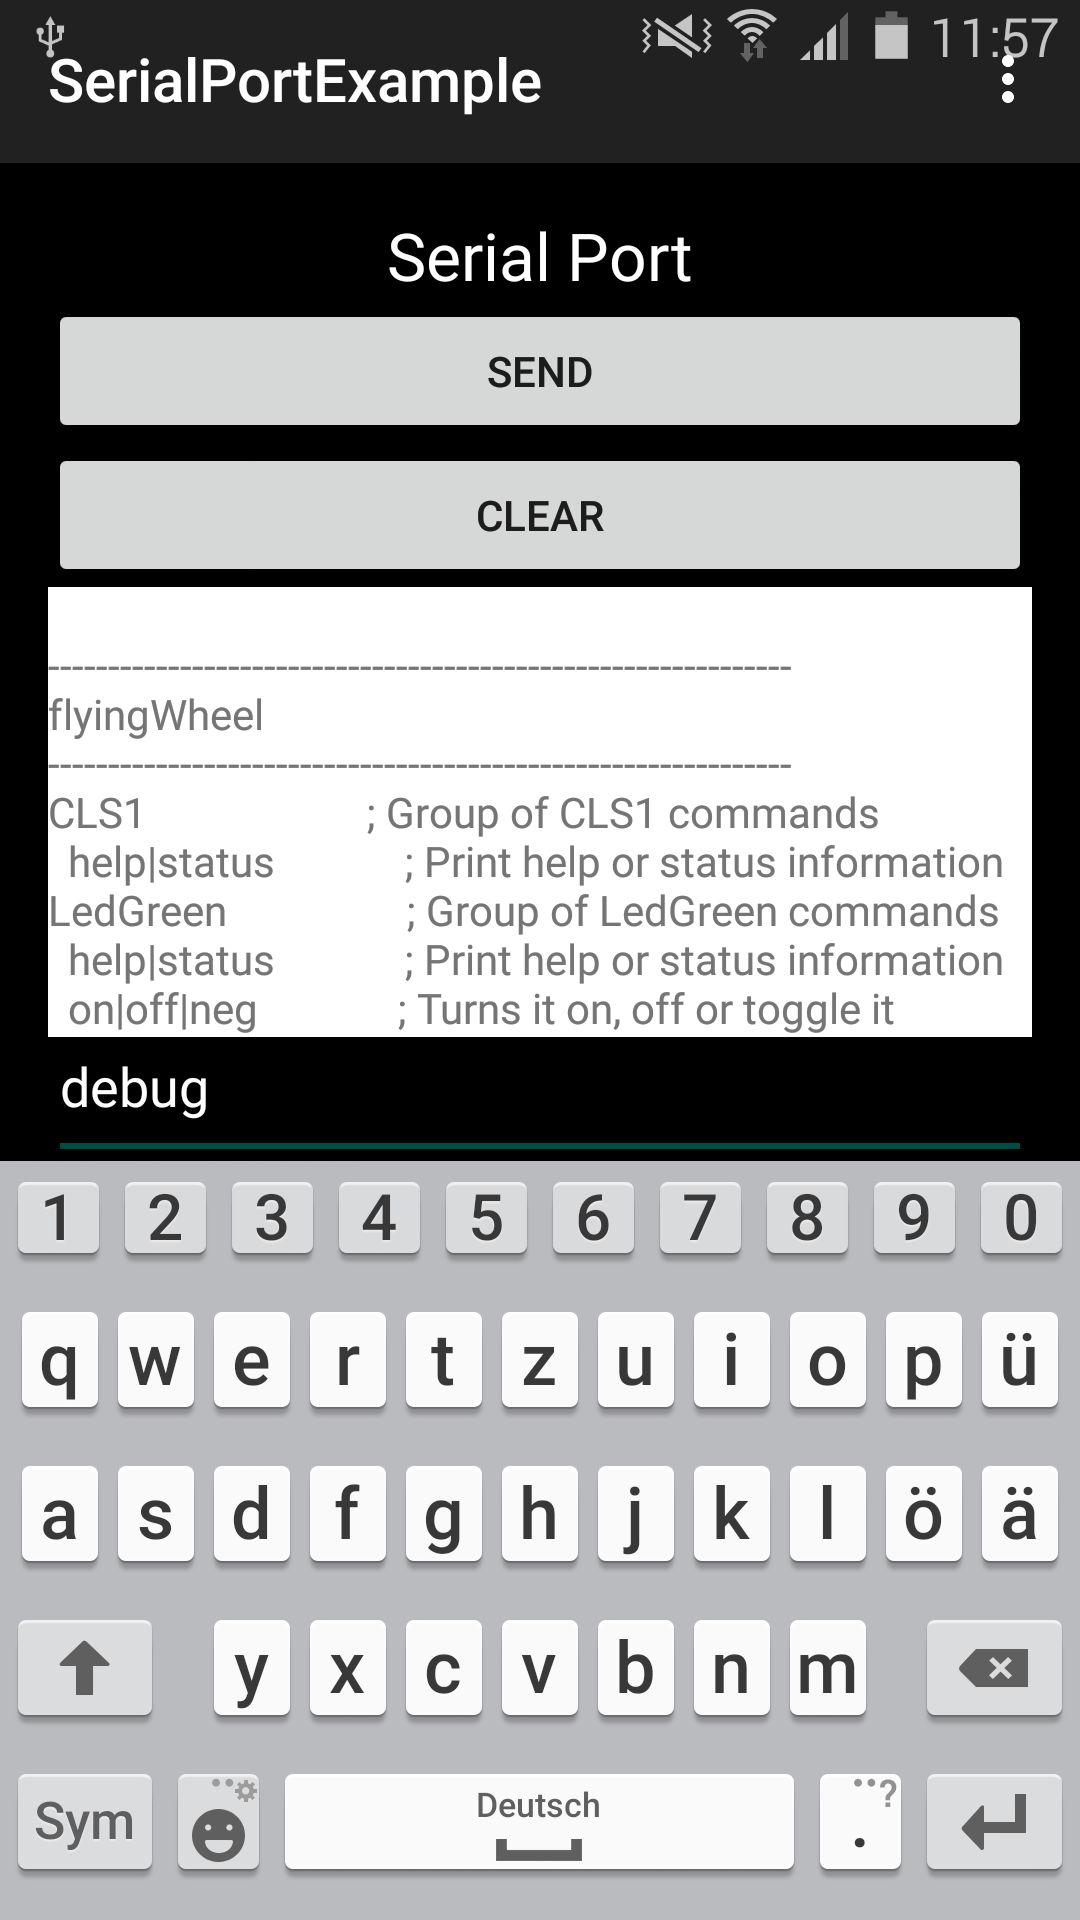
\includegraphics[width=0.3\textwidth,clip,trim=0mm 0mm 0mm 0mm]
	{Enddokumentation/Bilder/Screenshot_SerialPortExample_debug.png}
	\centering
	\caption{Screenshot Prototypen-App zur USB Kommunikation}
	\label{abb:ScreenshotSerialPortExample}
\end{figure}

Nach einem Update Mitte Februar 2015 durch den Entwickler der support-library funktioniert die App nun 
in bidirektionaler Richtung ohne Einschränkungen. Teil des Updates (respektive einziger Grund) war die 
Erweiterung der unterstützten Geräte um die CH34xSerialDevice-Schnittstelle. Damit erklärt sich auch das 
Fehlverhalten der  App vor dem Update, als die Bits nur bruchstückweise richtig geparst wurden. Es lag 
an der damals schon vorhandenen Schnittstelle zu der CDC-Geräte-Gruppe\footnote{Communication Device Class}, 
die nicht alle Geräte voll, sondern nur teilweise unterstütze. Zu einem dieser nicht vollumfänglich 
unterstützen Typen gehörte das Freedom-Board.
Der Code aus dem  Prototyp-App wird nun gewissermassen als Komponente zur Kommunikation mit dem USB-Gerät
im Android-App verwendet. 
\newline
\newline
Die Logik und Auslösung der Befehle an die Motoren findet vom Android-App via Freedom-Board statt. 
Damit sind das Starten der Brushless-DC-Motoren, das Ausrichten des Geräts mit dem Schrittmotor und das Starten 
des Motors für das Förderband gemeint. Nach dem Ausführen ihrer Aufgabe müssen die betreffeden Motoren 
ausgeschaltet werden, das wiederum vom Android-Phone aus passiert.\newline
Es wird ein fixes Protokoll und persistente asynchrone Kommunikation verwendet.
Die Verbindung ist unidirektional vom Android-Phone zum Freedom-Board. 
Als Befehle werden Strings im ASCII-Format an das Freedom-Board gesendet. Bespiele von Befehlen sind im Kapitel
\ref{sec:WinkelzuBoard} zu finden.


    \subsection{Camera}
Als weiteren Baustein der Android-App wird eine Kamera benötigt. Es stehen zurzeit 
zwei Kamera Frameworks von Android zur Verfügung. Das eine Framework ist die (deprecated)‚ 
'Camera', die seit dem Android API-Level\footnote{Application Programming Interface} 1 Teil des 
Android Development Kits ist.
\newline
\begin{figure}[h!]
	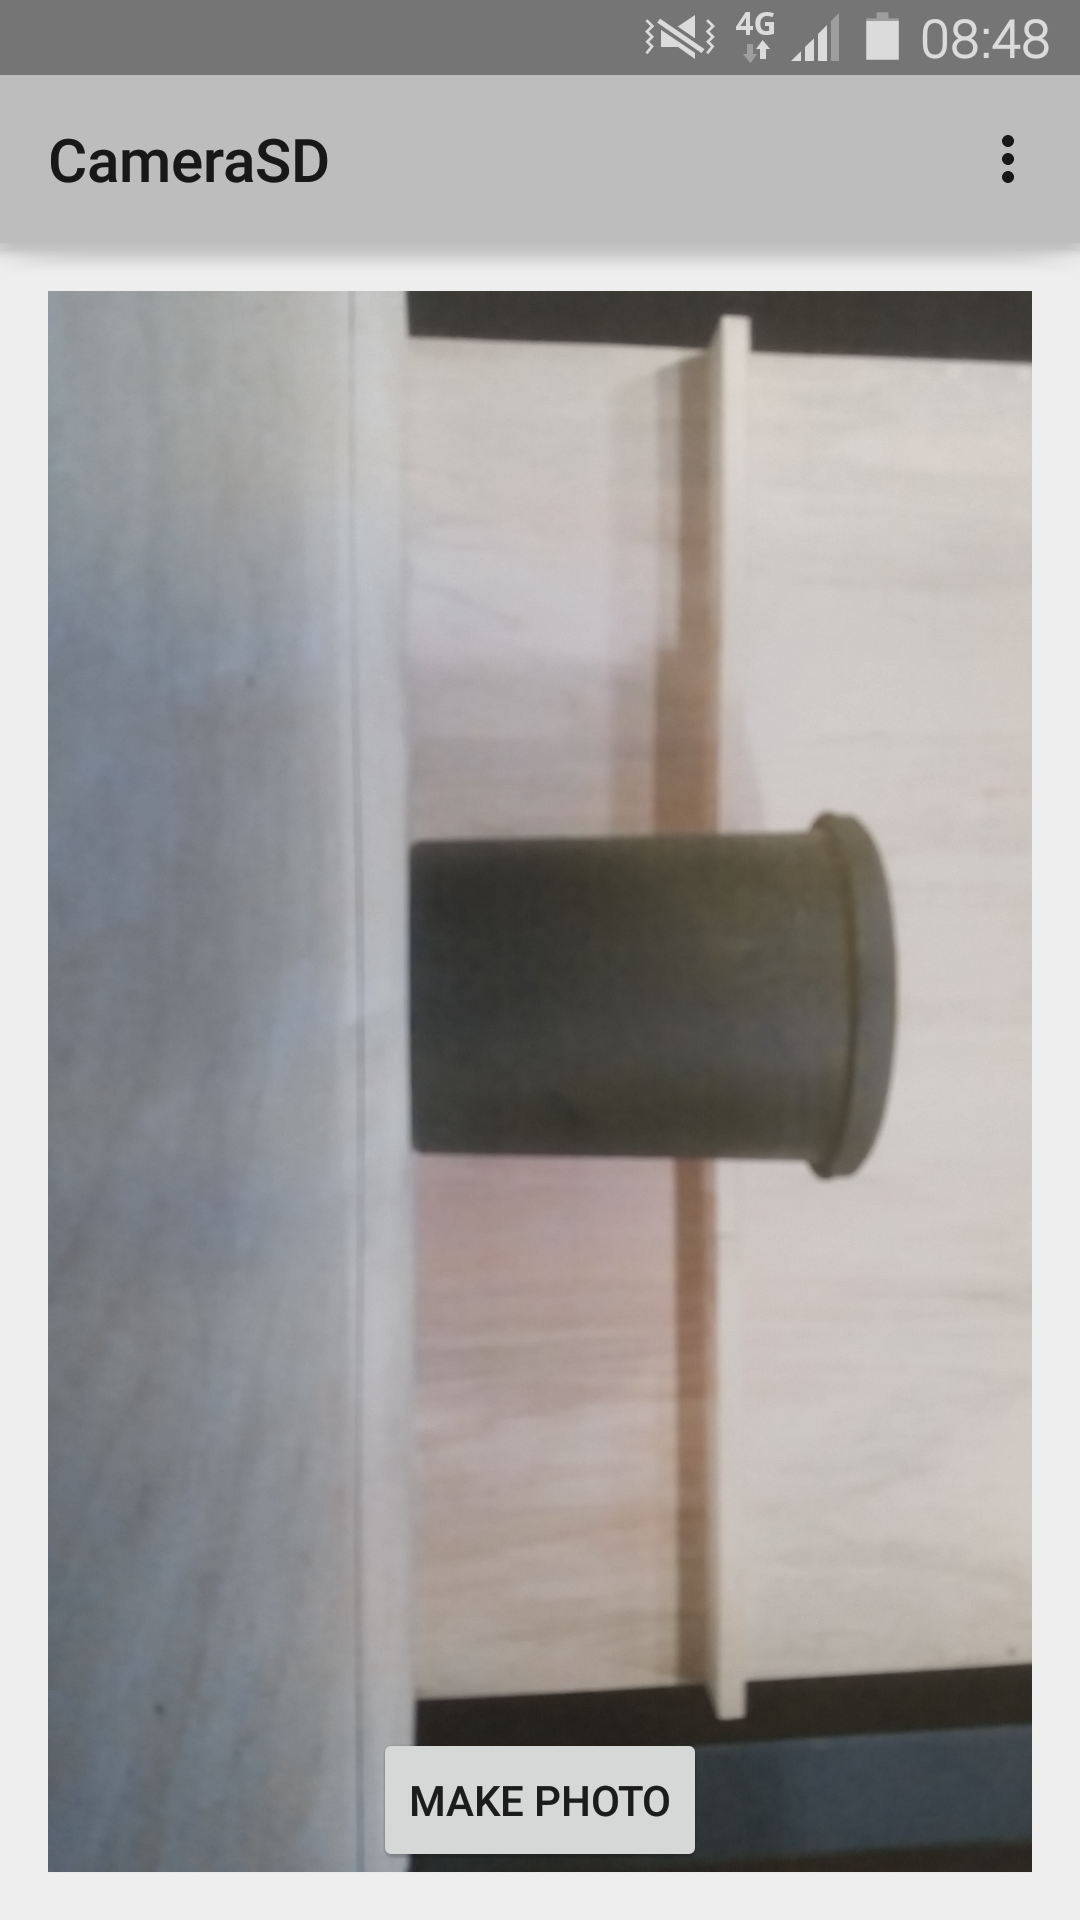
\includegraphics[width=0.3\textwidth,clip,trim=0mm 0mm 0mm 0mm]
	{Enddokumentation/Bilder/Screenshot_CameraSD.png}
	\centering
	\caption{Screenshot Camera Prototypen-App}
	\label{abb:ScreenshotCameraSD}
\end{figure}
Das andere Framework ist die Neue, ab API Level 21 verfügbare‚ 
 \enquote{Camera2}. Um die beiden Camera-Typen zu untersuchen, testen und vergleichen, wurden je eine App programmiert.
Im Vergleich der beiden Frameworks zeigte sich, dass die Entwicklung einer App mit dem alten Camera-Typ 
einiges speditiver von statten geht und der Code viel verständlicher ist. Die Entscheidung fiel deshalb 
auf das zwar veraltete aber erprobte  \enquote{Camera}-Framework.
\newline
\newline
Erst nach dem Test der beiden Applikationen konnte das Informatik-Team das Gerät für den PREN-Wettkampf festlegen. 
Da dieses Gerät auf Android Jelly Bean (API Level 17) basiert, schliesst dies die Verwendung 
der  \enquote{Camera2} (ab API Level 21) aus.

    \clearpage
    \section{Horizontale Ausrichtung}
	
    Um die Abwurfeinheit zum Zielkorb auszurichten, wird ein verstellbarer Mechanismus benötigt, 
    mit einer sehr hohe Genauigkeit. Der Drehpunkt befindet sich unter den Beschleunigungsrädern, 
    damit die Position des Abwurfes im Zentrum des Spielfeldes bleibt. Die Drehbewegung erfolgt 
    mittels eines Schrittmotores. Die Ausführung des Schrittmotores ist sehr flach gewählt, damit 
    der Schwerpunkt der ganzen Konstruktion auch tiefer gelegt werden kann. Dies ist notwendig, 
    damit die ganze Ballmaschine eine grössere Stabilität aufweist. Der Schrittmotor kann eine 
    Haltemoment von 0.083\si{\newton\meter} halten. Dies ist genügend gross, um die ganze 
    Abwurfeinheit in der gewünschten Zeit zu bewegen und bei der Position zu halten. Durch den 
    Schrittmotor kann eine sehr genaue Ansteuerung vorgenommen werden. Der Schrittmotor wird in der Abwurfeinheit angebracht und treibt ein Ritzel an, welches in einen Zahnkranz in der Grundplatte 
    eingreift. Die Grundplatte besteht auch aus einem Kreissegment von ??55\si{\degree}?? 
    mit einem Zahnrad vom Modul 1. Das Ritzel am Motor besteht aus 32 Zähnen. Es ist aus einer 
    6\si{\milli\meter} dicken MDF\footnote{mitteldichte Faserplatte} gelasert worden, damit es auf 
    das die Motorenachse aufgepresst werden konnte. Dies ist mit Acrylglas nicht möglich da dieses 
    Material zu spröde ist. Dadurch kann die Abwurfeinheit gedreht werden. Dies ist in Abbildung 
    \ref{abb:} ersichtlich. Damit die Bauhöhe nicht zusätzlich 
    vergrössert wird, ist der Zahnkranz in die Bodenplatte integriert. Um die Drehachse ist ein Kreis 
    mit dem Durchmesser der Breit vom Abwurfmechanismus integriert worden, welcher eine Abstützung 
    der ganzen Ballmaschine dient.\\
    Damit der Schrittmotor keine hohes Drehmoment aufweisen muss, sind am Ende des Wurfmechanismus 
    zwei Kugellager angebracht, welche die Drehbewegung übernehmen. Dadurch ist die Reibung bei der 
    Drehbewegung sehr klein. Die Lagerung erfolgt im Drehzentrum durch eine Hülse.


     \subsection{Ansteuerung Steppermotor}
        Die Ansteuerung des Stepper-Motors erfolgt über die entwickelte Hardware der PREN-ET-Gruppe. 
        Dieses Board kann direkt auf das Freedom-Board aufgesteckt und über die Konsole bedient 
        werden. Die gesamte Dokumentation dazu ist im Anhang \ref{apx:} angefügt. 
        
        \subsubsection{Auflösung}
        \label{sec:Aufloesung}
            Eine Umdrehung des Steppers benötigt 200 Vollschritte. Das Stepper-Board ist so konfiguriert, 
            dass $1:128$ Microstepping verwendet wird. Das gewählte Übersetzungsverhältnis vom 
            Stepper ist $1:28$ und somit ergeben sich die folgenden Auflösungen:
            \begin{equation}
                128 \cdot 200 \cdot 28 = 716'800\frac{\text{Microsteps}}{360\si{\degree}}
            \end{equation}
            \begin{equation}
                \frac{365\si{\degree}}{716'800} = 509 \cdot 10^{-6}\frac{\si{\degree}}{\text{Microsteps}}
            \end{equation}
            \begin{equation}
               \frac{1\si{\degree}}{509 \cdot 10^{-6}\frac{\si{\degree}}{\text{Microsteps}}} = 1963.8\frac{\text{Microsteps}}{\si{\degree}}
            \end{equation}
            
    \clearpage
    \section{Förderband}
\label{sec:Foerderband}
	Da die Beschleunigungsräder durch den Abwurf abgebremst werden, müssen 
	sie nach jedem Wurf wieder auf Nenndrehzahl gebracht werden. Um dafür 
	genügend Zeit zu haben, erfolgt die Zuführung der Bälle in zeitlichen 
	Abständen. Ein weiteres Kriterium für eine konstante Wurfweite, ist eine 
	gleichbleibende Geschwindigkeit mit der die Bälle zwischen die 
	Beschleunigungsräder kommen. Der Antrieb des Förderbandes erfolgt mit 
	einem DC-Motor, siehe Kapitel \ref{sec:FoerderbandAnsteuerung}. Die 
	Drehzahl ist mittels einer Zahnradpaarung mit $i=5$ übersetzt, um das 
	benötigte Drehmoment an die Antriebswelle des Förderbandes zu übertragen. 
	Die Antriebswelle und die Achse sind einteilig aus Aluminium gedreht. 
	Welle und Achse sind mittels Kugellager in den Seitenplatten gelagert. 
	Die Auflagefläche des Riemens auf der Antriebswelle ist bombiert gefertigt. 
	Dadurch wird ein seitliches Abrutschen des Riemens im Betrieb verhindert. 
	Auf dem Förderband, welches ein Flachbandriemen ist, sind Führungsschaufeln 
	angebracht, siehe Abbildung \ref{abb:Foerderband}. Durch den Abstand dieser 
	Schaufeln, ergeben sich die kurzen 
	Pausen um die Motoren hochzudrehen. Die Führungsschaufeln sind so 
	ausgerundet, dass der Ball möglichst lange geführt werden kann ohne die 
	Beschleunigungsräder zu berühren. Die Schaufeln sind aus $1\si{\milli\meter}$ 
	Aluminium Blech gefertigt und wurden auf dem Riemen aufgeklebt. Bei den 
	Testversuchen stellte sich heraus, dass durch die aufgeklebten Schaufeln 
	der Riemen nicht rund läuft. Jedes Mal wenn eine Klebestelle die Achse 
	passierte, erhöhte sich der Widerstand und das Band drehte langsamer. 
	Ausserdem hat der Endlosriemen an der Stelle an der er gefügt ist eine 
	höhere Steifigkeit, was denselben Effekt hatte. Ausgehend von diesen 
	Erkenntnissen wurde der Riemen neu gefertigt. Die Schaufeln wurden nicht 
	mehr geklebt, sondern mit einem Faden angenäht. Dazu wurden in Riemen 
	und Führungsschaufeln je drei Bohrungen gemacht und mit verstärktem Faden 
	Verbunden. So sind die Führungsschaufeln nur noch mit einer Linienverbindung 
	und nicht mehr mit einer Flächenverbindung auf dem Riemen befestigt. An 
	der Fügestelle des Riemens wurde in Längsrichtung Material entnommen, was 
	eine Verringerung der Steifigkeit bewirken sollte. In den nachfolgenden 
	Testversuchen zeigten die Anpassungen ihre gewünschte Wirkung. Die 
	Geschwindigkeit während einer Umdrehung war nun annähernd konstant. Aus 
	diversen Testversuchen der Ballzuführung während PREN1 wurde erkannt, dass 
	für einen idealen Abwurf die Tennisbälle mit beiden Beschleunigungsräder 
	gleichzeitig in Kontakt kommen müssen. Somit ist es notwendig die Bälle 
	zunächst unter dem oberen Beschleunigungsrad hindurch und anschliessend in 
	einem 45\si{\degree} Winkel nach oben zuzuführen. Dazu dient ein Führungselement, 
	siehe Abbildung \ref{abb:Abschusswinkel}
	welches auf beiden Seiten des Acrylglases angebracht ist. Diese 
	Führungselemente sind an die Form der Tennisbälle angepasst und mittels 
	3D Druck hergestellt worden. 
	\begin{figure}[h!]
    	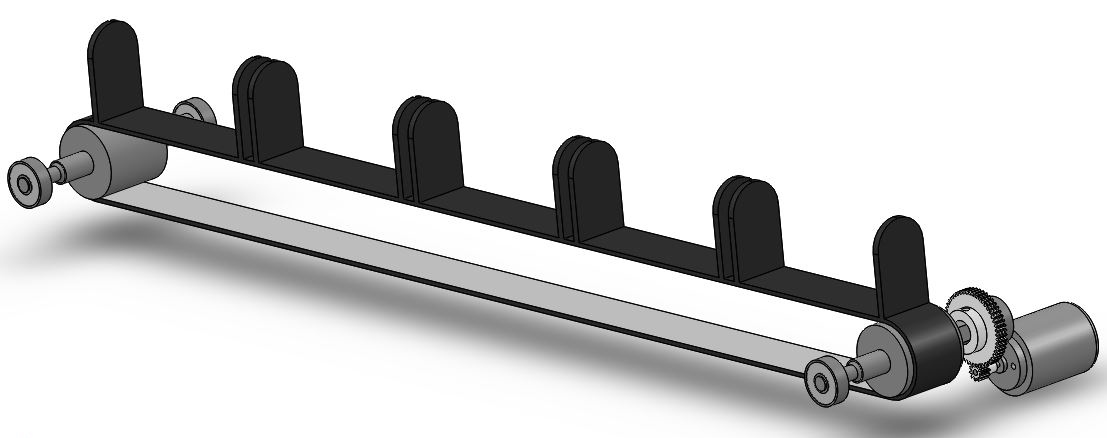
\includegraphics[width=0.9\textwidth,clip,trim=0mm 0mm 0mm 0mm]
    	{Enddokumentation/Bilder/Foerderband.jpg}
    	\centering
    	\caption{Aufbau des Förderbandes}
    	\label{abb:Foerderband}
 	\end{figure}

\subsection{Ansteuerung DC-Motor}
\label{sec:FoerderbandAnsteuerung}
    Die Ansteuerung des Motors, der das Förderband antreibt, erfolgt mittels PWM. Auf diese 
    Weise lässt sich die Drehzahl und somit die Nachführgeschwindigkeit einstellen. Das 
    Band muss nur in eine Richtung angetrieben werden, wodurch die Ansteuerung einfacher 
    realisiert werden kann. Das Schema ist in Abbildung \ref{abb:SchemaAnsteuerung} 
    ersichtlich. Im wesentlichen besteht diese Ansteuerung aus einem Vortreiber und einem 
    Schalter. Der Treiber bewirkt ein möglichst schnelles und effizientes Öffnen und Schliessen des Schalters. Auf diese Weise reduziert man die Schaltverluste. 
    \begin{figure}[h!]
    	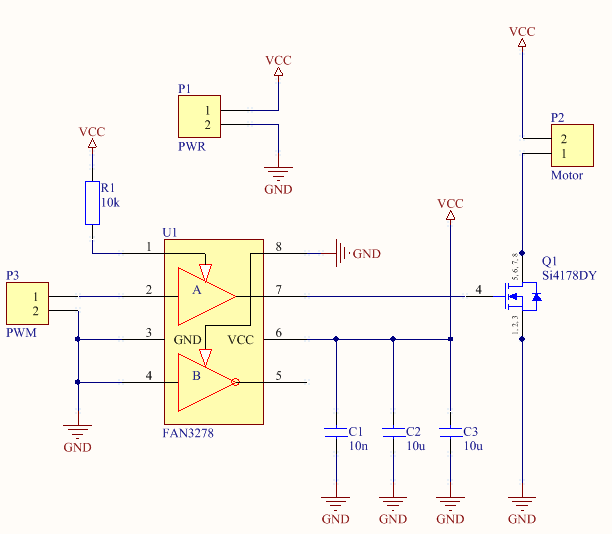
\includegraphics[width=0.7\textwidth,clip,trim=0mm 2mm 0mm 7mm]
    	{Enddokumentation/Bilder/Schema_DC-Ansteuerung.png}
    	\centering
    	\caption{Schema des Förderbandansteuerung}
    	\label{abb:SchemaAnsteuerung}
    \end{figure}
    \section{Beschleunigungsräder}
    Die Vortriebskraft für die Tennisbälle wird durch zwei Beschleunigungsräder gewährleistet. Der verwendete
    Beschleunigungsradantrieb wurde aus mehreren Gründen gewählt. Über die Drehzahl und den 
    Anpressdruck der Räder kann die Wurfweite stufenlos eingestellt werden. Somit ist die Maschine 
    für jeden Tennisball in einem bestimmten Bereich gewappnet. Die Beschleunigungsräder wurden 
    aus PVC hergestellt, da dieser Werkstoff einfach zu bearbeiten ist und zugleich eine genügend 
    grosse Festigkeit bietet. Um möglichst viel Gewicht zu sparen, wurde an beiden Planflächen so 
    viel Material wie möglich herausgenommen. Für die Übertragung des Momentes auf die Welle wurde 
    ein Presssitz realisiert. Dies ermöglicht eine gleichmässige Flächenpressung und erhöht die 
    Rundlaufgenauigkeit gegenüber einer geklebten Welle-Nabe-Verbindung. Weiter ist durch die konkave Form der 
    Beschleunigungsräder die Richtung der Ballflugbahn vorgegeben. Hier wird keine zusätzliche Ballführung 
    gebraucht was Gewicht, Kosten und Platz spart. Die Räder sind konkav ausgearbeitet, so dass die 
    Beschleunigung nicht nur über einen Punkt übertragen wird. So wird gewährleistet, dass die Kraft 
    über eine grössere Fläche übertragen wird. Dadurch entsteht wiederum der Vorteil, dass die 
    Beschleunigung geführt abläuft, wodurch ein gerichteter Wurf entsteht. So kann die vorhandene 
    Rotationsenergie vollumfänglich den Tennisbällen übergeben werden. Die Ausrundung wird durch 
    den Radius der Bälle gegeben. Der Durchmesser der Beschleunigungsräder ist so festgelegt, dass 
    mit der vorhandenen Masse ein genügendes Trägheitsmoment zur Verfügung steht. Dies ist nötig, 
    damit bei der Beschleunigung der Tennisbälle die Räder nicht zu stark abgebremst werden. Durch 
    den Durchmesser wird auch die Winkelgeschwindigkeit festgelegt. Zudem sind die Räder mit einer 
    speziellen Haftmatte beschichtet, damit die 
    Kraft optimal auf den Ball übertragen werden kann. Dies ist in Abbildung \ref{abb:BeschleunigungsräderMitHaftmatte} ersichtlich. Somit wird ein höherer Haftreibungskoeffizient 
    erreicht und Schlupf zwischen Bällen und Beschleunigungsräder verhindert. Die Achsen der zwei Beschleunigungsräder sind im 
    Winkel von 45\si{\degree} zur Bodenplatte angeordnet, siehe Abbildung \ref{abb:Abschusswinkel}. 
    Der Abschusswinkel ist so gewählt, dass 
    die Tennisbälle mit einem genügend grossen Einschlagwinkel im Zielbereich landen. So wird die 
    Möglichkeit einer Kollision mit dem Korbrand vermieden.
    \begin{figure}[h!]
       	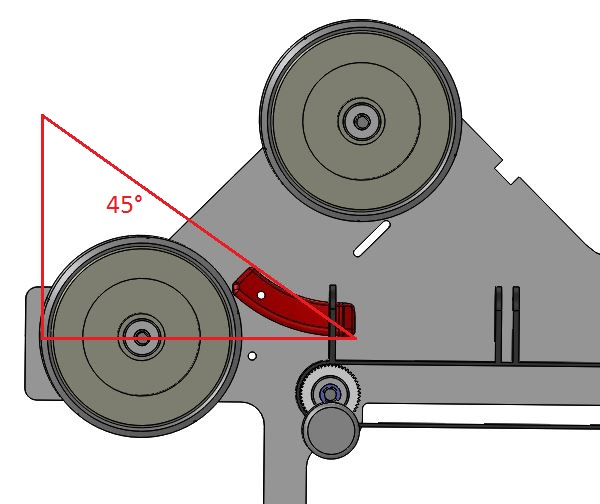
\includegraphics[width=0.5\textwidth,clip,trim=20mm 5mm 0mm 5mm]
       	{Enddokumentation/Bilder/Abschuss.JPG}
       	\centering
       	\caption{Ballzuführung mit Abschusswinkel}
       	\label{abb:Abschusswinkel}
    \end{figure}
    %    
     \begin{figure}[h!]
     	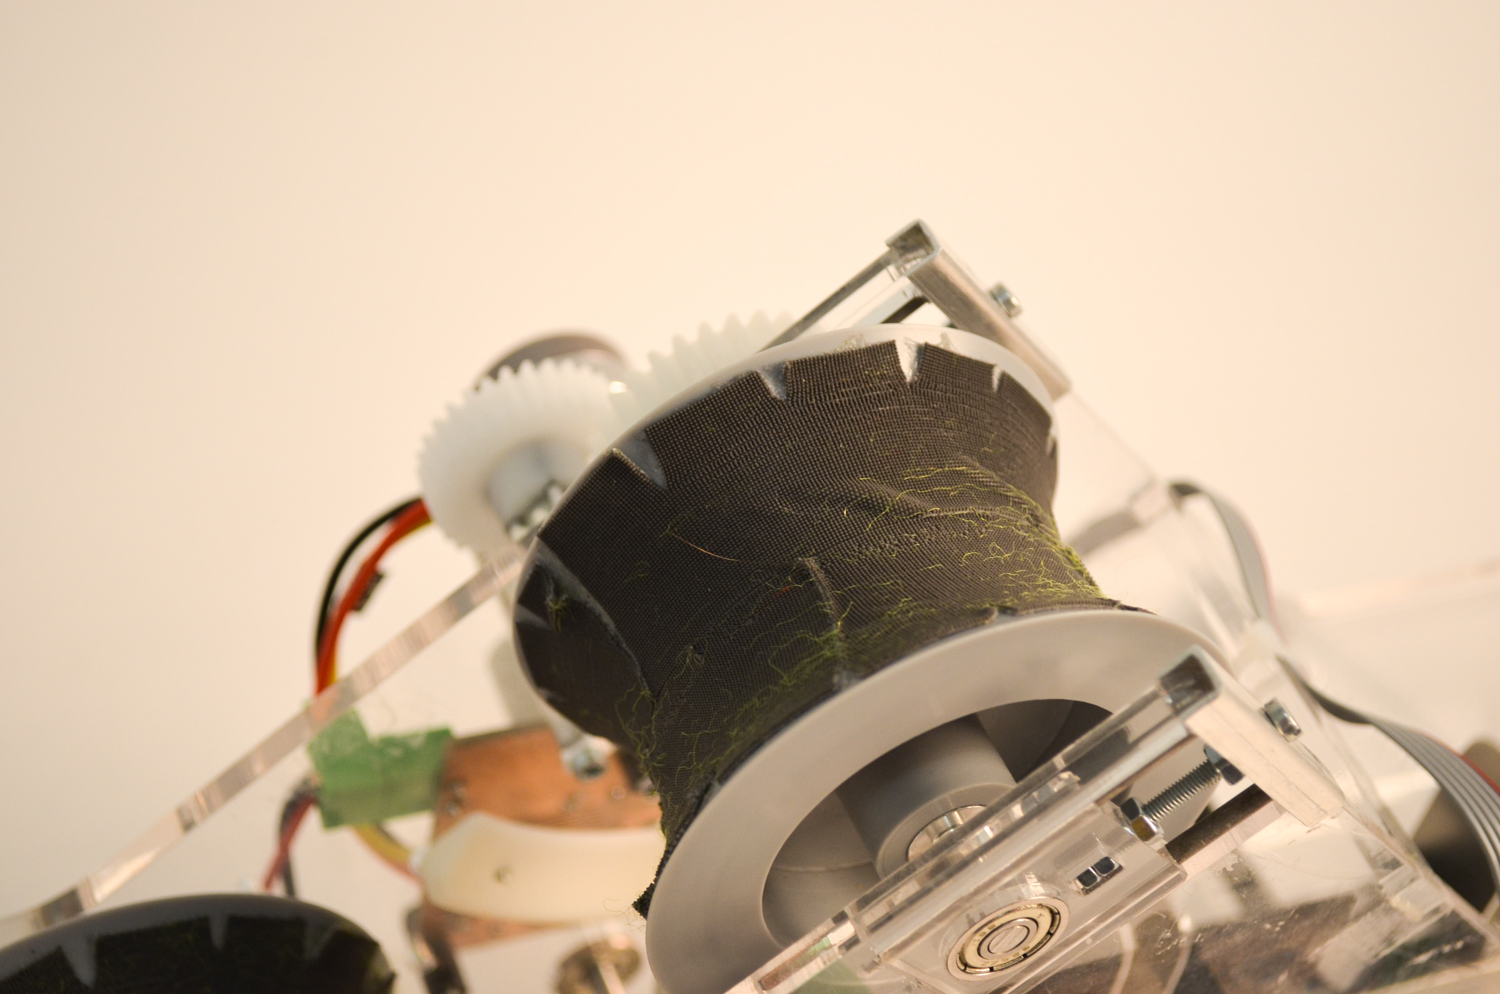
\includegraphics[width=0.5\textwidth,clip,trim=20mm 0mm 0mm 5mm]
     	{Enddokumentation/Bilder/Haftmatte.JPG}
     	\centering
     	\caption{Beschleunigungsräder mit Haftmatte}
     	\label{abb:BeschleunigungsräderMitHaftmatte}
     \end{figure}
    
    \subsection{Antriebsstrang}
        Für die Übertragung der Momente der Brushlessmotoren auf die Beschleunigungsräder wurde eine 
        Zahnradübersetzung von $1:4$ gewählt.
		\begin{figure}[h!]
			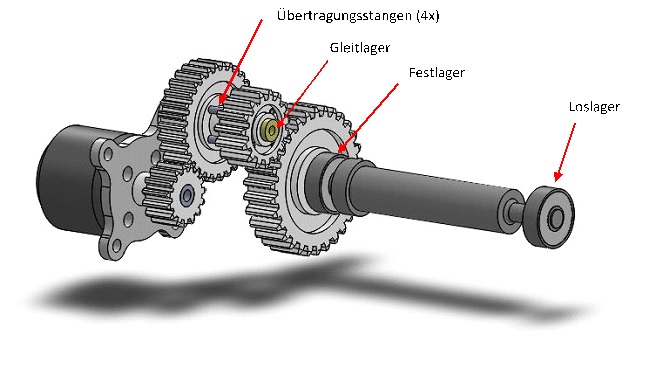
\includegraphics[width=0.9\textwidth,clip,trim=0mm 15mm 0mm 0mm]
			{Enddokumentation/Bilder/Antriebsstrang.JPG}
			\centering
			\caption{Der Antriebsstrang}
			\label{abb:Antriebsstrang}
		\end{figure}
        \begin{table}[h!]
            \centering
            \begin{zebratabular}{p{0.10\textwidth}p{0.25\textwidth}}
                \rowcolor{gray} Anzahl & Beschreibung\\
                \rule{0pt}{11pt}2x & Brushlessmotor \\
                \rule{0pt}{11pt}2x & Zahnrad Modul 1.0 Z15\\
                \rule{0pt}{11pt}2x & Zahnrad Modul 1.0 Z30\\
                \rule{0pt}{11pt}2x & Zahnrad Modul 1.25 Z15\\
                \rule{0pt}{11pt}2x & Zahnrad Modul 1.25 Z30\\
            \end{zebratabular}
            \caption{Zahnräder der Übersetzung}
            \label{tab:AntriebsstrangKraft}
        \end{table}
        Auf die Welle des Brushlessmotores wurde eine Büchse eingepresst, da die Standardbohrung des 
        Zahnrades grösser als die des Wellendurchmessers war. Das Zahnrad selber wurde ebenfalls auf die 
        Büchse aufgepresst und noch zusätzlich mit einer Stellschraube fixiert. Das grosse Zahnrad, 
        der Welle der Beschleunigungsräder, wurde ebenfalls nach dem gleichen Schema 
        montiert. Auch hier kam eine Einpressbüchse zum Einsatz und das Zahnrad wurde wiederum mit 
        einer Stellschraube fixiert. Für das Zahnradpaar in der Mitte der Übertragung brauchte es eine 
        zusätzliche Achse. Diese wurde mit zwei Schrauben an der Seitenwand des 
        Acrylglases und an der Motorbefestigungsplatte festgemacht. Die Achse ist fest und dient als 
        Gleitlager. Für die Übertragung der beiden Zahnräder auf dem Gleitlager wurden vier kleine Stangen 
        aus Aluminium verwendet, wobei das Gleitlager selbst ebenfalls aus Aluminium besteht. Die Welle der 
        Beschleunigungsräder ist als Fest- und Loslager ausgeführt. Das Festlager befindet sich auf 
        der Seite des Zahnrades und ist gegen axiales Verschieben mit einem Sicherungsring versehen. 
        Das Übersetzungsverhältnis $i$ berechnet sich wie folgt, der Index 1 bezieht sich dabei auf 
        das Zahnrad am Brushlessmotor.
        \begin{equation}
            i = i_1 \cdot i_2 = \frac{z_2}{z_1} \cdot \frac{z_4}{z_3} = \frac{30}{15} \cdot \frac{30}{15} = 4
        \end{equation}
%
%Ab hier ist es die ET-Doku. Die Files sind Kopien, der Master liegt im ET-Repo
\subsection{Ansteuerung}
Die folgenden Unterkapitel \ref{sec:ET_Hardware} und \ref{sec:ET_Firmware} sind wie im PREN1 \cite{Team32:Doku} in Zusammenarbeit mit der ET-Gruppe erstellt worden. 

Elektrotechnik-Studierende aus mehreren Gruppen haben sich
zusammengeschlossen um gemeinsame Probleme anzugehen. Dabei handelt es sich
um die benötigte Hard- und Software, um Motoren anzusteuern
und gegebenenfalls zu regeln. In diesem Zusammenschluss werden drei Gruppen
gebildet, um Lösungen für DC-, Stepper- und Brushless-Motoren auszuarbeiten.
Die Idee besteht darin, dass nicht jede Gruppe für dasselbe Problem wo
möglich denselben Lösungsansatz verfolgt, sondern die Ressourcen kombiniert,
Synergien nutzt, um eine bessere Lösung zu erarbeiten. Auf diese Weise kann
das teamübergreifende Arbeiten im Rahmen des PREN erlernt und
geübt werden. Somit wird Idee der Interdisziplinarität im erweiterten Sinn
Rechnung getragen. Die Gruppen und deren Mitglieder sind in Tabelle 
\ref{tab:pren-et-overview} aufgeführt.
\begin{table}[h!]
	\centering
	\begin{zebratabular}{l l}
		\rowcolor{gray} Projekt		& Team \\
		DC Motoren   & 33, 39 \\
		Schrittmotor & 27, 33, 38 \\
		BLDC Motor   & 27, 32 \\
	\end{zebratabular}
	\caption{Übersicht der PREN-ET Projektgruppen}
	\label{tab:pren-et-overview}
\end{table}


\ifSTANDALONE
\section{Hardware}
\fi
\ifEMBED
\subsubsection{Hardware}
\label{sec:ET_Hardware}
\fi
\ifSTANDALONE
\subsection{Übersicht}
\fi
\ifEMBED
\paragraph{Übersicht}$~~$\vspace{2mm}\\
\fi
Der Aufbau der Ansteuerung der BLDC-Motoren ist als Blockschaltbild in Abbildung 
\ref{abb:BlockschaltbildBLDC} ersichtlich.\\
\begin{figure}[h!]
   	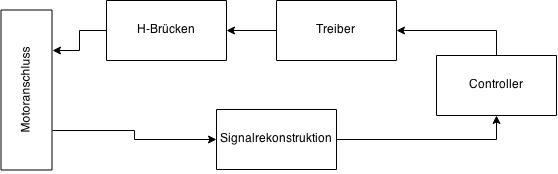
\includegraphics[width=0.8\textwidth,clip,trim=0mm 0mm 0mm 0mm]
   	{\EtPath/Bilder/Blockschaltbild_BLDC.jpg}
   	\centering
   	\caption{Blockschaltbild des BLDC-Boards}
   	\label{abb:BlockschaltbildBLDC}
\end{figure}\\
In der Abbildung \ref{abb:BlockschaltbildBLDCPhoto} ist die Realisierung der Blöcke ersichtlich. 
Dabei ist der erste Kasten der Anschluss des Motors, der zweite die H-Brücken, der dritte der 
Treiber, der vierte die Signalrekonstruktion und der fünfte Teil ist der Controller, auf dem 
die Firmware läuft.
\begin{figure}[h!]
   	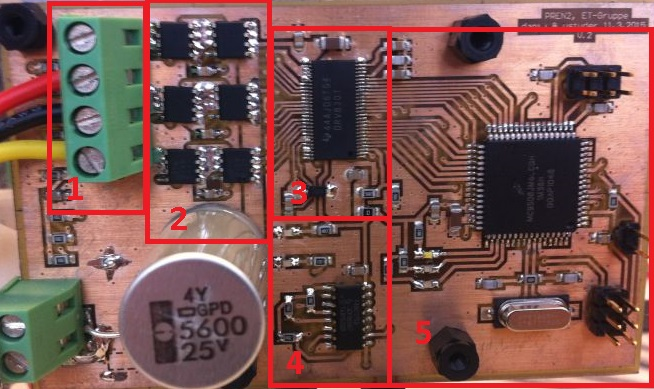
\includegraphics[width=0.8\textwidth,clip,trim=0mm 0mm 0mm 0mm]
   	{\EtPath/Bilder/BLDC-BoardBloecke.jpg}
   	\centering
   	\caption{Blockschaltbild des BLDC-Boards}
   	\label{abb:BlockschaltbildBLDCPhoto}
\end{figure}

\ifSTANDALONE
\subsection{Kommutierung}
\fi
\ifEMBED
\paragraph{Kommutierung}$~~$\vspace{2mm}\\
\fi
Der Motor wird mit drei Halbbrücken kommutiert. Für die Ansteuerung der MOSFET\footnote{metal-oxide-semiconductor field-effect transistor} 
wird ein Predriver DRV8301 von Texas Instruments eingesetzt. Die Halbbrücken 
werden einzeln vom Controller geschalten. Damit nur ein 
PWM\footnote{\textbf{P}ulse \textbf{W}idth \textbf{M}odulation}-Signal erzeugt 
werden muss, werden die Ansteuerleitungen mittels Widerständen mit dem 
PWM-Signal verbunden. Werden die Ansteuerungen vom Controller nicht aktiv 
getrieben, liegt die PWM an. Die Konfiguration der Predrivers erfolgt über SPI. 

\ifSTANDALONE
\subsection{Phasendetektion}
\fi
\ifEMBED
\paragraph{Phasendetektion}$~~$\vspace{2mm}\\
\fi
Die Phasendetektion besteht aus Sternpunktnachbildung, Komparator und 
Synchronisation. Die Sternpunktnachbildung erzeugt einen virtuellen Sternpunkt 
mit Hilfe eines Widerstandsnetzwerkes und eines Tiefpassfilters. Die einzelnen 
Phasenspannungen werden mit diesem virtuellen Sternpunkt verglichen. Mit einem 
Flipflop wird das Signal mit der PWM Synchronisiert. 

\ifSTANDALONE
\subsection{Controller}
\fi
\ifEMBED
\paragraph{Controller}$~~$\vspace{2mm}\\
\fi
Als Controller kommt ein HC9S08JM60 der Firma Freescale zum Einsatz. Der Takt 
wird mittels Quarz mit 12MHz erzeugt. Um den aktuellen Betriebsszustand 
anzuzeigen, stehen drei LED zur Verfügung. 

\ifSTANDALONE
\subsection{Speisung}
\fi
\ifEMBED
\paragraph{Speisung}$~~$\vspace{2mm}\\
\fi
Die Eingangsspannung wird mittels eines optional bestückbaren Filters von 
Murata gefiltert. Der Predriver wird direkt mit dieser gefilterten Speisung 
betrieben. Mit dem im Predriver integrierten Step-Down-Converter wird eine 
Spannung von 3.3\si{\volt} erzeugt. Für Varianten mit hoher Betriebsspannung (>30\si{\volt}) 
wird der Komparator der Phasendetektion über einen diskret aufgebauten 
Spannungsregler mit einer Spannung von 30\si{\volt} versorgt. 


\ifSTANDALONE
\section{Firmware}
\fi
%\ifEMBED
%\subsection{Firmware}
%\fi

\subsection{Übersicht}

\ifSTANDALONE
\subsection{Takt}
\fi
\ifEMBED
\subsubsection{Takt}
\fi
Der Referenztakt wird durch einen Quarz mit einer Frequenz von 
12\si{\mega\hertz} erzeugt.  Dieser Takt dient als Referenztakt für die PLL 
des HS9S08JM60. Dazu wird er durch 8 geteilt um im erlaubten 
Bereich\footnote{Die Frequenz des Eingangssignals der PLL muss im Bereich 1 
\ldots 2\si{\mega\hertz} liegen. \cite[p.  195]{Datasheet:HCS08}} für die PLL 
zu liegen. In der PLL wird der Takt mit 32 multipliziert. Dies ergibt einen 
CPU Takt von 48\si{\mega\hertz}. Da der Bustakt der Hälfte des CPUtakts 
entspricht, weist dieser eine Frequenz von 24\si{\mega\hertz} auf.  Der 
Externe Takt (16\si{\mega\hertz}) wird zusätzlich als externer Referenztakt 
zur Verfügung gestellt und vom RTC verwendet.  (siehe auch Abschnitt 
\ref{sec:rtc} \nameref{sec:rtc})

\ifSTANDALONE
\subsection{RTC}
\fi
\ifEMBED
\subsubsection{RTC}
\fi
\label{sec:rtc}
Um regelmässig abzuarbeitende Aufgaben zu steuern, wird ein entsprechender 
Takt benötigt. Dafür wird der RTC\footnote{\textbf{R}eal \textbf{T}ime 
\textbf{Counter}} verwendet. Dieser verwendet als Takt den externen 
Referenztakt mit einer Frequenz von 16\si{\mega\hertz}. Dieser wird mit dem 
Prescaler auf eine Frequenz von 16\si{\kilo\hertz} geteilt. Über das Modulo 
Register kann eine Periodendauer im Bereich 62.5\si{\micro\second} \ldots 
16\si{\milli\second} eingestellt werden. Es wird zunächst eine Periodendauer 
von 1\si{\milli\second} verwendet. In der ISR\footnote{\textbf{I}nterrupt 
\textbf{S}ervice \textbf{Routine}} wird ein Flag gesetzt, welches in der 
Hauptschlaufe abgefragt wird. 
\begin{table}[h!]
    \begin{zebratabular}{p{0.10\textwidth}p{0.06\textwidth}p{0.25\textwidth}p{0.5\textwidth}}
    \rowcolor{gray} Register & Wert & Beschreibung & Bemerkungen \\
    RTCSC &
        \verb!0x38! &
        RTC Status and Control Register &
        ERCLK, Interrupts enabled, Prescaler = $10^3$ $\to$ T$_{\text{Count}}$ = $\frac{1}{16}$\si{\milli\second} \\
    RTCMOD &
        \verb!0x0F! &
        RTC Modulo Register &
        Modulo = 15 $\to$ T$_{\text{Interrupt}}$ = 1\si{\milli\second} \\
    \end{zebratabular}
    \caption{Registerinitialisierung RTC}
    \label{tab:rtc_init}
\end{table}

\subsection{PWM}
Mit der PWM\footnote{\textbf{P}ulse \textbf{W}idth \textbf{M}odulation} werden 
die Ausgangsstufen angesteuert. Über das Puls - Pausenverhältnis wird die 
Leistung eingestellt. Damit diese Ansteuerung jedoch nicht hörbar wird, muss 
der Motor mit einer PWM Frequenz oberhalb des hörbaren Frequenzbereichs des 
Menschen angesteuert werden. Es wird eine Frequenz von 24\si{\kilo\hertz} 
verwendet.  Für das Erzeugen der PWM wird der Timer TPM2 verwendet. 
\begin{table}[h!]
    \begin{zebratabular}{p{0.10\textwidth}p{0.06\textwidth}p{0.25\textwidth}p{0.5\textwidth}}
    \rowcolor{gray} Register & Wert & Beschreibung & Bemerkungen \\
    TPM2SC &
        \verb!0x08! &
        TPM2 Status and Control Register &
        Overflow interrupt disabled, no Center-aligned PWM, Bus clock as clock 
            source, Prescaler = 1\\
    TPM2CNT &
        \verb!0x____! &
        TPM2 Counter Register &
        No initialisation \\
    TPM2MOD &
        \verb!0x03FF! &
        TPM2 Counter Modulo Register &
        1023 $\to$ $\frac{24\si{\mega\hertz}}{1024} = 23.4375\si{\kilo\hertz}$  \\
    TPM2C0SC &
        \verb!0x28! &
        TPM2 Channel 0 Status and Control Register &
        Interrupt disabled, edge aligned PWM, High-true\\
    TPM2C0V &
        \verb!0x0033! &
        TPM2 Channel 0 Value Register &
        5\si{\percent} \\
    TPM2C1SC &
        \verb!0x24! &
        TPM2 Channel 1 Status and Control Register &
        Interrupt disabled, edge aligned PWM, Low-true\\
    TPM2C1V &
        \verb!0x03CD! &
        TPM2 Channel 1 Value Register &
        5\si{\percent} \\
    \end{zebratabular}
    \caption{Registerinitialisierung TPM2}
    \label{tab:rtc_init}
\end{table}

\ifSTANDALONE
\subsection{Kommutierungsverzögerung / Zeitmessung}
\fi
\ifEMBED
\subsubsection{Kommutierungsverzögerung / Zeitmessung}
\fi
Um den exakten Kommutierungszeitpunkt einstellen zu können, und um die Zeit 
zwischen zwei Kommutierungen zu messen wird ein weiterer Timer benötigt. Dafür 
wird TPM1 verwendet. Als Taktquelle für den Timer wird der Bustakt mit einer 
Frequenz von 24\si{\mega\hertz} verwendet. Dieser wird mit dem maximal möglichen 
Prescaler von 128 geteilt. Dies ergibt eine Frequenz von 187.5\si{\kilo\hertz} 
und eine Auflösung von 5.33\si{\micro\second}. Damit ist eine maximale 
Messdauer von 349.5\si{\milli\second} möglich. 
\begin{table}[h!]
    \begin{zebratabular}{p{0.10\textwidth}p{0.06\textwidth}p{0.25\textwidth}p{0.5\textwidth}}
    \rowcolor{gray} Register & Wert & Beschreibung & Bemerkungen \\
    TPM1SC &
        \verb!0x0F! &
        TPM1 Status and Control Register &
        Overflow interrupt disabled, no Center-aligned PWM, Bus clock as clock 
            source, Prescaler = 128\\
    TPM1CNT &
        \verb!0x____! &
        TPM1 Counter Register &
        No initialisation \\
    TPM1MOD &
        \verb!0x0000! &
        TPM1 Counter Modulo Register &
        Free running \\
    TPM1C0SC &
        \verb!0x50! &
        TPM1 Channel 0 Status and Control Register &
        Interrupt enabled, Output compare \\
    TPM1C0V &
        \verb!0x0000! &
        TPM1 Channel 0 Value Register &
        Used for commutation delay of phase U \\
    TPM1C1SC &
        \verb!0x50! &
        TPM1 Channel 1 Status and Control Register &
        Interrupt enabled, Output compare \\
    TPM1C1V &
        \verb!0x0000! &
        TPM1 Channel 1 Value Register &
        Used for commutation delay of phase V \\
    TPM1C2SC &
        \verb!0x50! &
        TPM1 Channel 2 Status and Control Register &
        Interrupt enabled, Output compare \\
    TPM1C2V &
        \verb!0x0000! &
        TPM1 Channel 2 Value Register &
        Used for commutation delay of phase W \\
    TPM1C3SC &
        \verb!0x44! &
        TPM1 Channel 3 Status and Control Register &
        Interrupt enable, input capture \\
    TPM1C3V &
        \verb!0x0000! &
        TPM1 Channel 3 Value Register &
        Initialized zero, value not used later \\
    TPM1C4SC &
        \verb!0x44! &
        TPM1 Channel 4 Status and Control Register &
        Interrupt enable, input capture \\
    TPM1C4V &
        \verb!0x0000! &
        TPM1 Channel 4 Value Register &
        Initialized zero, value not used later \\
    TPM1C5SC &
        \verb!0x44! &
        TPM1 Channel 5 Status and Control Register &
        Interrupt enable, input capture \\
    TPM1C5V &
        \verb!0x0000! &
        TPM1 Channel 5 Value Register &
        Initialized zero, value not used later \\
    \end{zebratabular}
    \caption{Registerinitialisierung TPM1}
    \label{tab:rtc_init}
\end{table}


\ifSTANDALONE
\subsection{Kommunikation zum Host}
\fi
\ifEMBED
\subsubsection{Kommunikation zum Host}
\fi
Zur Interaktion mit dem BLDC-Board wird die SPI1-Schnittstelle des $\mu C$ verwendet. Dabei
ist das SPI-Interface im 8 Bit Mode mit LSB-First konfiguriert. Zusätzlich zu dieser Schnittstelle
ist eine IRQ-Leitung vorhanden, mit der das BLDC-Board den Host triggern kann, um auf ein Problem 
hinzuweisen. Die Steckerbelegung ist in Tabelle \ref{tab:SPI_stecker} ersichtlich.
\begin{table}[h!]
    \begin{zebratabular}{p{0.10\textwidth}p{0.06\textwidth}p{0.25\textwidth}p{0.5\textwidth}}
    \rowcolor{gray} Register & Wert & Beschreibung & Bemerkungen \\
    SPI1C2 &
        \verb!0x00! &
        SPI Control Register 2 & 
        \\
    SPI1C1 &
        \verb!0x85! &
        SPI Control Register 1 &
        IRQ-Enable aktiviert und LSB-First konfiguriert\\
    \end{zebratabular}
    \caption{Registerinitialisierung SPI1}
    \label{tab:spi1_init}  
\end{table}

\begin{table}[h!]
    \begin{zebratabular}{p{0.10\textwidth}p{0.06\textwidth}}
    \rowcolor{gray} Pin & Name\\
    1 & GND\\
    2 & MISO\\
    3 & CS\\
    4 & MOSI\\
    5 & CLK\\
    6 & IRQ\\
    \end{zebratabular}
    \centering
    \caption{Steckerbelegung der SPI-Schnittstelle}
    \label{tab:SPI_stecker}
\end{table}
Die Kommunikation zwischen BLDC-Board und Host funktioniert über ein Protokoll zur Interaktion. die 
Spezifikation dieses ist in der Tabelle \ref{tab:Spi_Int_Table} ersichtlich. Das obere Nibble des
CMD's enthält den Befehl und das untere Nibble die Anzahl Argumente, die zum CMD gehören.
Wenn das untere Nibble \verb!0xF! ist, wird die Länge der Übertragung im nächsten Byte signalisiert.
\begin{table}[h!]
    \begin{zebratabular}{p{0.12\textwidth}p{0.06\textwidth}p{0.35\textwidth}p{0.4\textwidth}}
    \rowcolor{gray} Name & Wert & Beschreibung & Parameter\\
    Dummy &
        \verb!0x00! & 
        Byte das benötigt wird, um zu clocken für die Übertragung von Argumenten &
        \\
    Start &
        \verb!0x10! & 
        Startet den Motor &
        \\
    Stop &
        \verb!0x20! & 
        Stoppt den Motor &
        \\
    setRPM &
        \verb!0x32! & 
        16 Bit Zahl um die Drehzahl einzustellen & 
        1. Byte = High-Byte\newline 
        2. Byte = Low-Byte\\
    setVoltage &
        \verb!0x42! & 
        $U_{GS}$ der FET's. & 1. Byte = Spannungswert-High-Byte\newline 
                              2. Byte = Spannungswert-Low-Byte\\
    setCurrent &
        \verb!0x51! & 
        Wert der Strombegrenzung. Der Stromwert ergibt sich nach der Formel $Current = Wert \cdot 10$ &
        $Registerwert = \frac{Sollwert\; in \;[mA]}{10} $\\
    getStatus &
        \verb!0x64! & 
        Gibt der Board-Status zurück &
        1. Byte = Motor-Status\newline
        2. Byte = Fehler-Code\newline
        3. Byte = RPM-High-Byte\newline
        4. Byte = RPM-Low-Byte\\
    areYouAlive &
        \verb!0x71! & 
        Damit kann die Kommunikation und das BLDC-Board testen &
        Das BLDC-Board gibt \verb!0x55! zurück\\
    setPwm &
        \verb!0x81! & 
        Damit kann die PWM des Motors eingestllt werden &
        PWM-Wert im Bereich 1-100 \% \\
    startMessung Param &
        \verb!0xC3! & 
        Messung parametrisiert starten &
        1. Byte = Pulsdauer\newline
        2. Byte = RPM-High-Byte\newline
        3. Byte = RPM-Low-Byte\\
    startMessung &
        \verb!0xD0! & 
        Messung mit einem Schritt starten &
        \\
    getMessung &
        \verb!0xEF! & 
        gibt die gespeicherte Messung zurück &
        1. Byte = Länge\newline
        2. - n. Byte = Daten der Messung\\
    \end{zebratabular}
    \caption{Kommunikationsprotokoll}
    \label{tab:Spi_Int_Table}
\end{table}



\begin{table}[h!]
    \begin{zebratabular}{p{0.07\textwidth}p{0.07\textwidth}p{0.07\textwidth}p{0.07\textwidth}p{0.07\textwidth}p{0.07\textwidth}p{0.07\textwidth}p{0.07\textwidth}}
    \rowcolor{gray} \multicolumn{8}{|c|}{Mögliche Werte als Argument für setVoltage }\\
    $60 mV$   & $68 mV$   & $76 mV$   & $86 mV$   & $97 mV$   & $109 mV$  & $123 mV$  & $138 mV$  \\
    $155 mV$  & $175 mV$  & $197 mV$  & $222 mV$  & $250 mV$  & $282 mV$  & $317 mV$  & $358 mV$  \\
    $403 mV$  & $454 mV$  & $511 mV$  & $576 mV$  & $648 mV$  & $730 mV$  & $822 mV$  & $926 mV$  \\
    $1046 mV$ & $1175 mV$ & $1324 mV$ & $1491 mV$ & $1679 mV$ & $1892 mV$ & $2131 mV$ & $2400 mV$ \\
    \end{zebratabular}
        \centering
    \caption{Gültige Wert als Argument für setVoltage}
\end{table}



    \clearpage
    \section{Projektplanung / -Management}

Das Projektteam 32 besteht aus sieben Personen, die sich auf folgende 
Studienrichtungen aufteilen: Drei Personen Maschinentechnik, drei 
Personen Informatik und eine Person Elektrotechnik. Die Studienrichtungen 
sind sogleich die jeweiligen Verantwortungen. In den Bereichen mit mehreren 
Projektmitgliedern wird die Verantwortung für Teilaufgaben jeweils 
situativ verteilt. Für allgemeine Projektarbeiten ist jeweils die 
hauptverantwortliche Person bestimmt. Diese kann Teilaufgaben definieren 
und sie an andere Teammitglieder zur Bearbeitung delegieren. Die Hierarchie 
im Team ist bewusst flach und ohne eigentlichen Projektleiter gehalten. 
Entscheide werden im Plenum diskutiert und gefällt. Die Leitung oder Führung 
einer Besprechung obliegt der oder den Verantwortlichen des jeweiligen Themas. 
Mit dieser Teamstruktur ist gewährleistet, dass alle Mitglieder Verantwortung 
tragen können und müssen. Dies soll Motivation und Eigeninitiative fördern. 
Im Verlauf von PREN1 hat sich gezeigt, dass diese Projektorganisation optimal 
ist. Jedes Teammitglied hatte das gleiche Mitspracherecht, was die Kreativität 
und das Engagement wesentlich förderte. Da kein eigentlicher Projektleiter 
vorhanden war, musste jedes Teammitglied über seinen Themenbereich hinaus 
mitdenken. Es entstand eine lebhafte Diskussionskultur, die viele gute Ansätze 
und Lösungen hervorbrachte. Da dies alles eher offen und frei vonstattenging, 
waren die Aufteilung und das Vorgehen danach nicht immer allen zu 100\% klar. 
Aus diesem Grund wurden in PREN2 die sogenannten Planungssitzungen eingeführt. 
Mit diesem Instrument wurden die Besprechungen und die Beschlussfassungen, die 
sich während PREN1 ergeben haben, organisierter und vor allem strukturierter durchgeführt.
Die Planungssitzungen wurden jeweils alle zwei bis drei Wochen abgehalten. An diesen 
Sitzungen wurden die Hauptaufgaben für die nächste Periode besprochen und 
festgehalten. Es wurde definiert, wer welche Arbeiten zu verrichten hat und welche 
Priorität diese haben. Weiter wurden Beschlüsse gefasst, Erkenntnisse und 
Auswirkungen der letzten Periode besprochen. Das Ganze wurde jeweils in einem 
Protokoll festgehalten (siehe Kapitel \ref{sec:BeginnRaporte}). Im Anschluss an 
die Planungssitzungen wurde jeweils auch das Risikomanagement besprochen und auf den 
neusten Stand gebracht. 
\newline
\newline
Die Projektplanung wurde nach demselben Muster wie in PREN1 geführt. Diese Excel 
Projektplanungsvorlage hat sich bewährt. Das Gantt-Diagramm ist einfach in der 
Handhabung und bietet eine grosse Übersichtlichkeit. Arbeiten welche im PREN1 
abgeschlossen wurden, sind übersichtshalber in dieser Planung nicht mehr 
aufgeführt. Allgemeine Projektarbeiten und Themengebiete, welche sich über beide 
Semester erstrecken, sind in die Planung von PREN2 übernommen worden. Um 
grösstmögliche Übersicht zu haben, ist die Projektplanung relativ allgemein 
gehalten. Das heisst, es sind alle Themen und Arbeitsblöcke vorhanden, jedoch 
ist nicht jeder einzelne Arbeitsschritt der darunter anfällt, auch aufgeführt. 
Ebenso ist jeweils nur die verantwortliche Person aufgelistet. Sie trägt die 
Hauptverantwortung über ein Arbeitsblock, jedoch können auch andere Personen 
daran gearbeitet haben. Die Zeitangaben, welche in Spalte drei enthalten sind, 
sind jeweils die Schätzungen, die im Voraus vom Verantwortlichen des Projektteiles 
gemacht wurden. Genaue Angaben über geleistete Arbeitszeit wie auch ein 
Soll-Istzeit Vergleich sind unter (siehe Kapitel \ref{sec:SollIstVergleich}) ersichtlich. 
Die Planung ist in einen Block allgemeine Projektarbeiten und einzelne Blöcke, welche die 
Disziplinen repräsentieren, unterteilt.
\begin{landscape}
\subsection{Zeitplan}    
    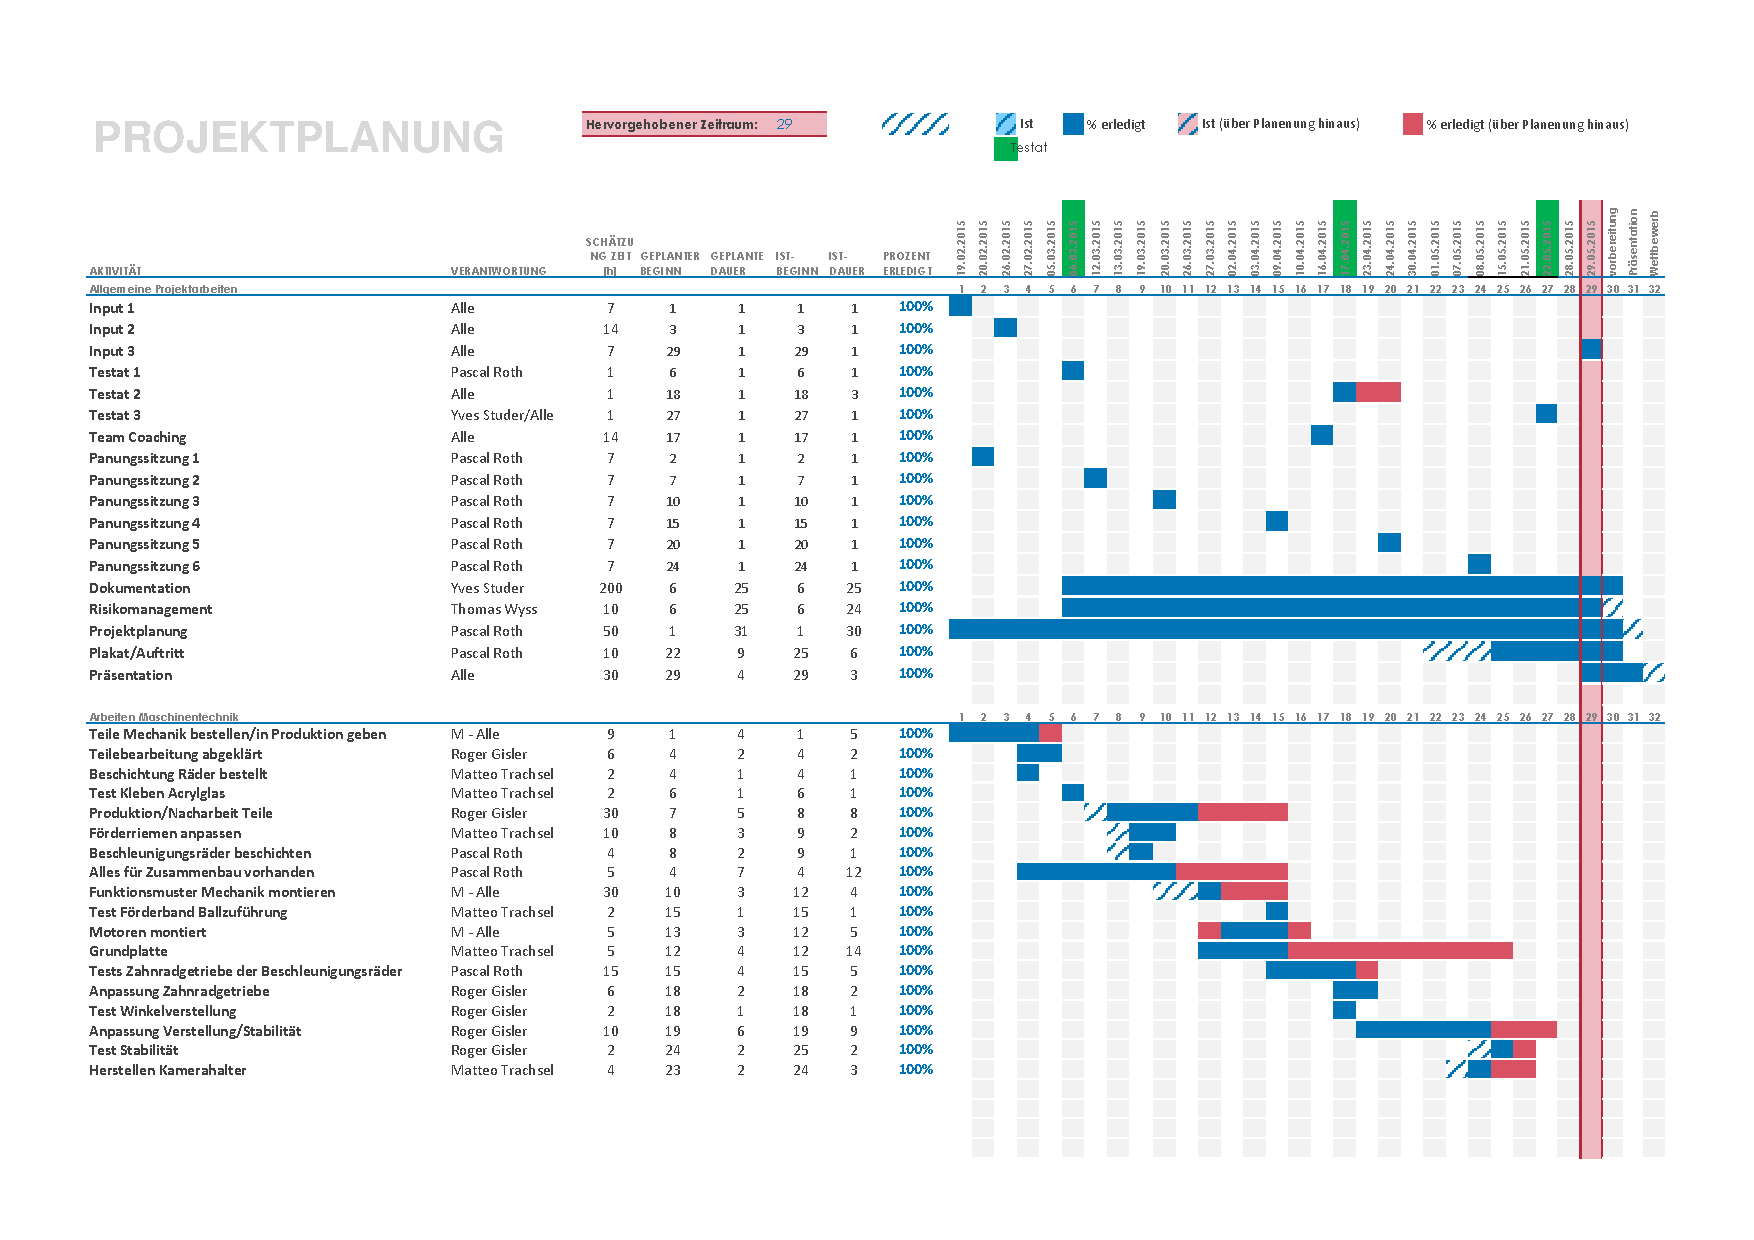
\includegraphics[page=1,scale=0.87,clip,trim=15mm 15mm 13mm 18mm] {Enddokumentation/Bilder/Projektplanung.pdf}
    \newpage        
    \includegraphics[page=2,scale=0.87,clip,trim=15mm 0mm 13mm 10mm] {Enddokumentation/Bilder/Projektplanung.pdf}
\end{landscape}

    \newpage
    \section{Schlussdiskussion}


    \subsection{Lessons Learned}
Eine wichtige Lektion hat das Informatik-Team bezüglich Vorhandensein einer nützlichen, 
konkreten Fallbacklösung (Dank vorhandenem Risikomanagement) für Schlüssel Technologien gelernt. 
Da eine zufriedenstellende Kommunikation mittels Bluetooth nicht gewährleistet werden konnte, 
musste auf die Fallback-Variante, die WLAN als Kommunikationsmittel verwendet, zurückgegriffen werden. 
Das Refactoring des Codes beanspruchte, im Vergleich zur aufgewendet Zeit für das Lösen des Bluetooth-Problems, 
signifikant weniger Zeit. Das Informatik-Team hätte den Umstieg auf die Fallback-Lösung früher einleiten sollen, 
dass hätte einiges an wertvoller Entwicklungszeit eingespart.
\newline
\newline
Als Kommunikationsmittel zwischen den Android-Phone und dem Desktop war anfangs PREN2 eine Verbindung 
mittels Bluetooth gedacht. Obwohl im PREN1 schon einzelne Test bezüglich verbinden der zwei Geräte und 
senden von Daten durchgeführt wurden, kam das Informatik-Team nicht umhin, das Konzept \enquote{Bluetooth} mit einem neuen 
Konzept zu ersetzen. Wie bereits in der Dokumentation des PREN1-Moduls beschrieben, war als Fallback-Lösung 
die Verwendung von WLAN gedacht. 
\\
\\
Die teamübergreifende Zusammenarbeit in der ET-Gruppe hat sich extrem bewährt.  Auf diese Weise 
konnte eine komplexere und anspruchsvolle Lösung realisiert werden. Dementsprechend war der 
Lerneffekt massiv grösser. Die ET-Zusammenarbeit hat sich nicht nur in der Erhöhung der man-power 
niedergeschlagen, sondern auch in der Vielfalt der Themen und deren spezifischen Problemen sowie 
Lösungen. Am Anfang war es zeitintensiv, die Gruppen, die Tools und das gemeinsame Vorgehen zu 
definieren und umzusetzen. Sobald dies erledigt war, funktionierte die Zusammenarbeit innerhalb 
der ET-Gruppe ausserordentlich gut.
    \newpage
    
    %Beginn Testberichte / Testprotokolle
    \section{Tests}
\subsection{Klebeversuch}
\begin{zebratabular}{p{4.5cm}p{\textwidth-5.3cm}}
	\rule{0pt}{11pt}\textit{Tester}           & Matteo Trachsel\\ 
	\rule{0pt}{11pt}\textit{Datum}:           & 06.03.2015\\
	\rule{0pt}{11pt}\textit{Beschreibung}:    & Das Ziel dieses Testes bestand darin, den 
												gekauften Kleber UHU Hart auf seine Klebekraft und auf sein Erscheinungsbild zu testen.\\
	\rule{0pt}{11pt}\textit{Akteure}:         & Acrylglas \\
	\rule{0pt}{11pt}\textit{Bedingung}:       & Für den Test werden verschiedene Acrylglas-Stücke zusammengeklebt.
	Hierfür wird der Kleber wie auf der Gebrauchsanweisung auf zwei Verfahren getestet. 
	Im ersten Versuch wird der UHU Kleber aufgetragen und die zwei Platten zusammengeklebt. 
	Im zweiten Versuch wird der Kleber zuerst auf die Acrylglasstücke aufgetragen und 
	gewartet bis er angetrocknet ist, danach noch einmal eine Schicht vom Kleber aufgetragen 
	und zusammengefügt.\\
	\rule{0pt}{11pt}\textit{Erwartete Fehlermeldung}:          & keine \\
	\rule{0pt}{11pt}\textit{Vorgehen}:        & Kleber auf Acrylglas, zusammenhalten \\
	\rule{0pt}{11pt}\textit{Erwartetes Ergebnis}: & Mit dem Versuch konnte gezeigt werden, dass der Kleber sicher glasklar bleibt. Weiter 
	ist die erwünschte Klebekraft bestätigt worden. Beim zweiten Versuch, wo zuerst der 
	Kleber etwas angetrocknet wurde, ist eine deutlich schlechtere Klebekraft festgestellt 
	worden. Dadurch wird der Kleber immer sofort aufgeklebt.\\
	\rule{0pt}{11pt}\textit{Eingetretenes Ergebnis}: & Alles IO.\\
	\rule{0pt}{11pt}\textit{Test bestanden?}:     & Ja \\
\end{zebratabular}  


\begin{figure}[h!]
	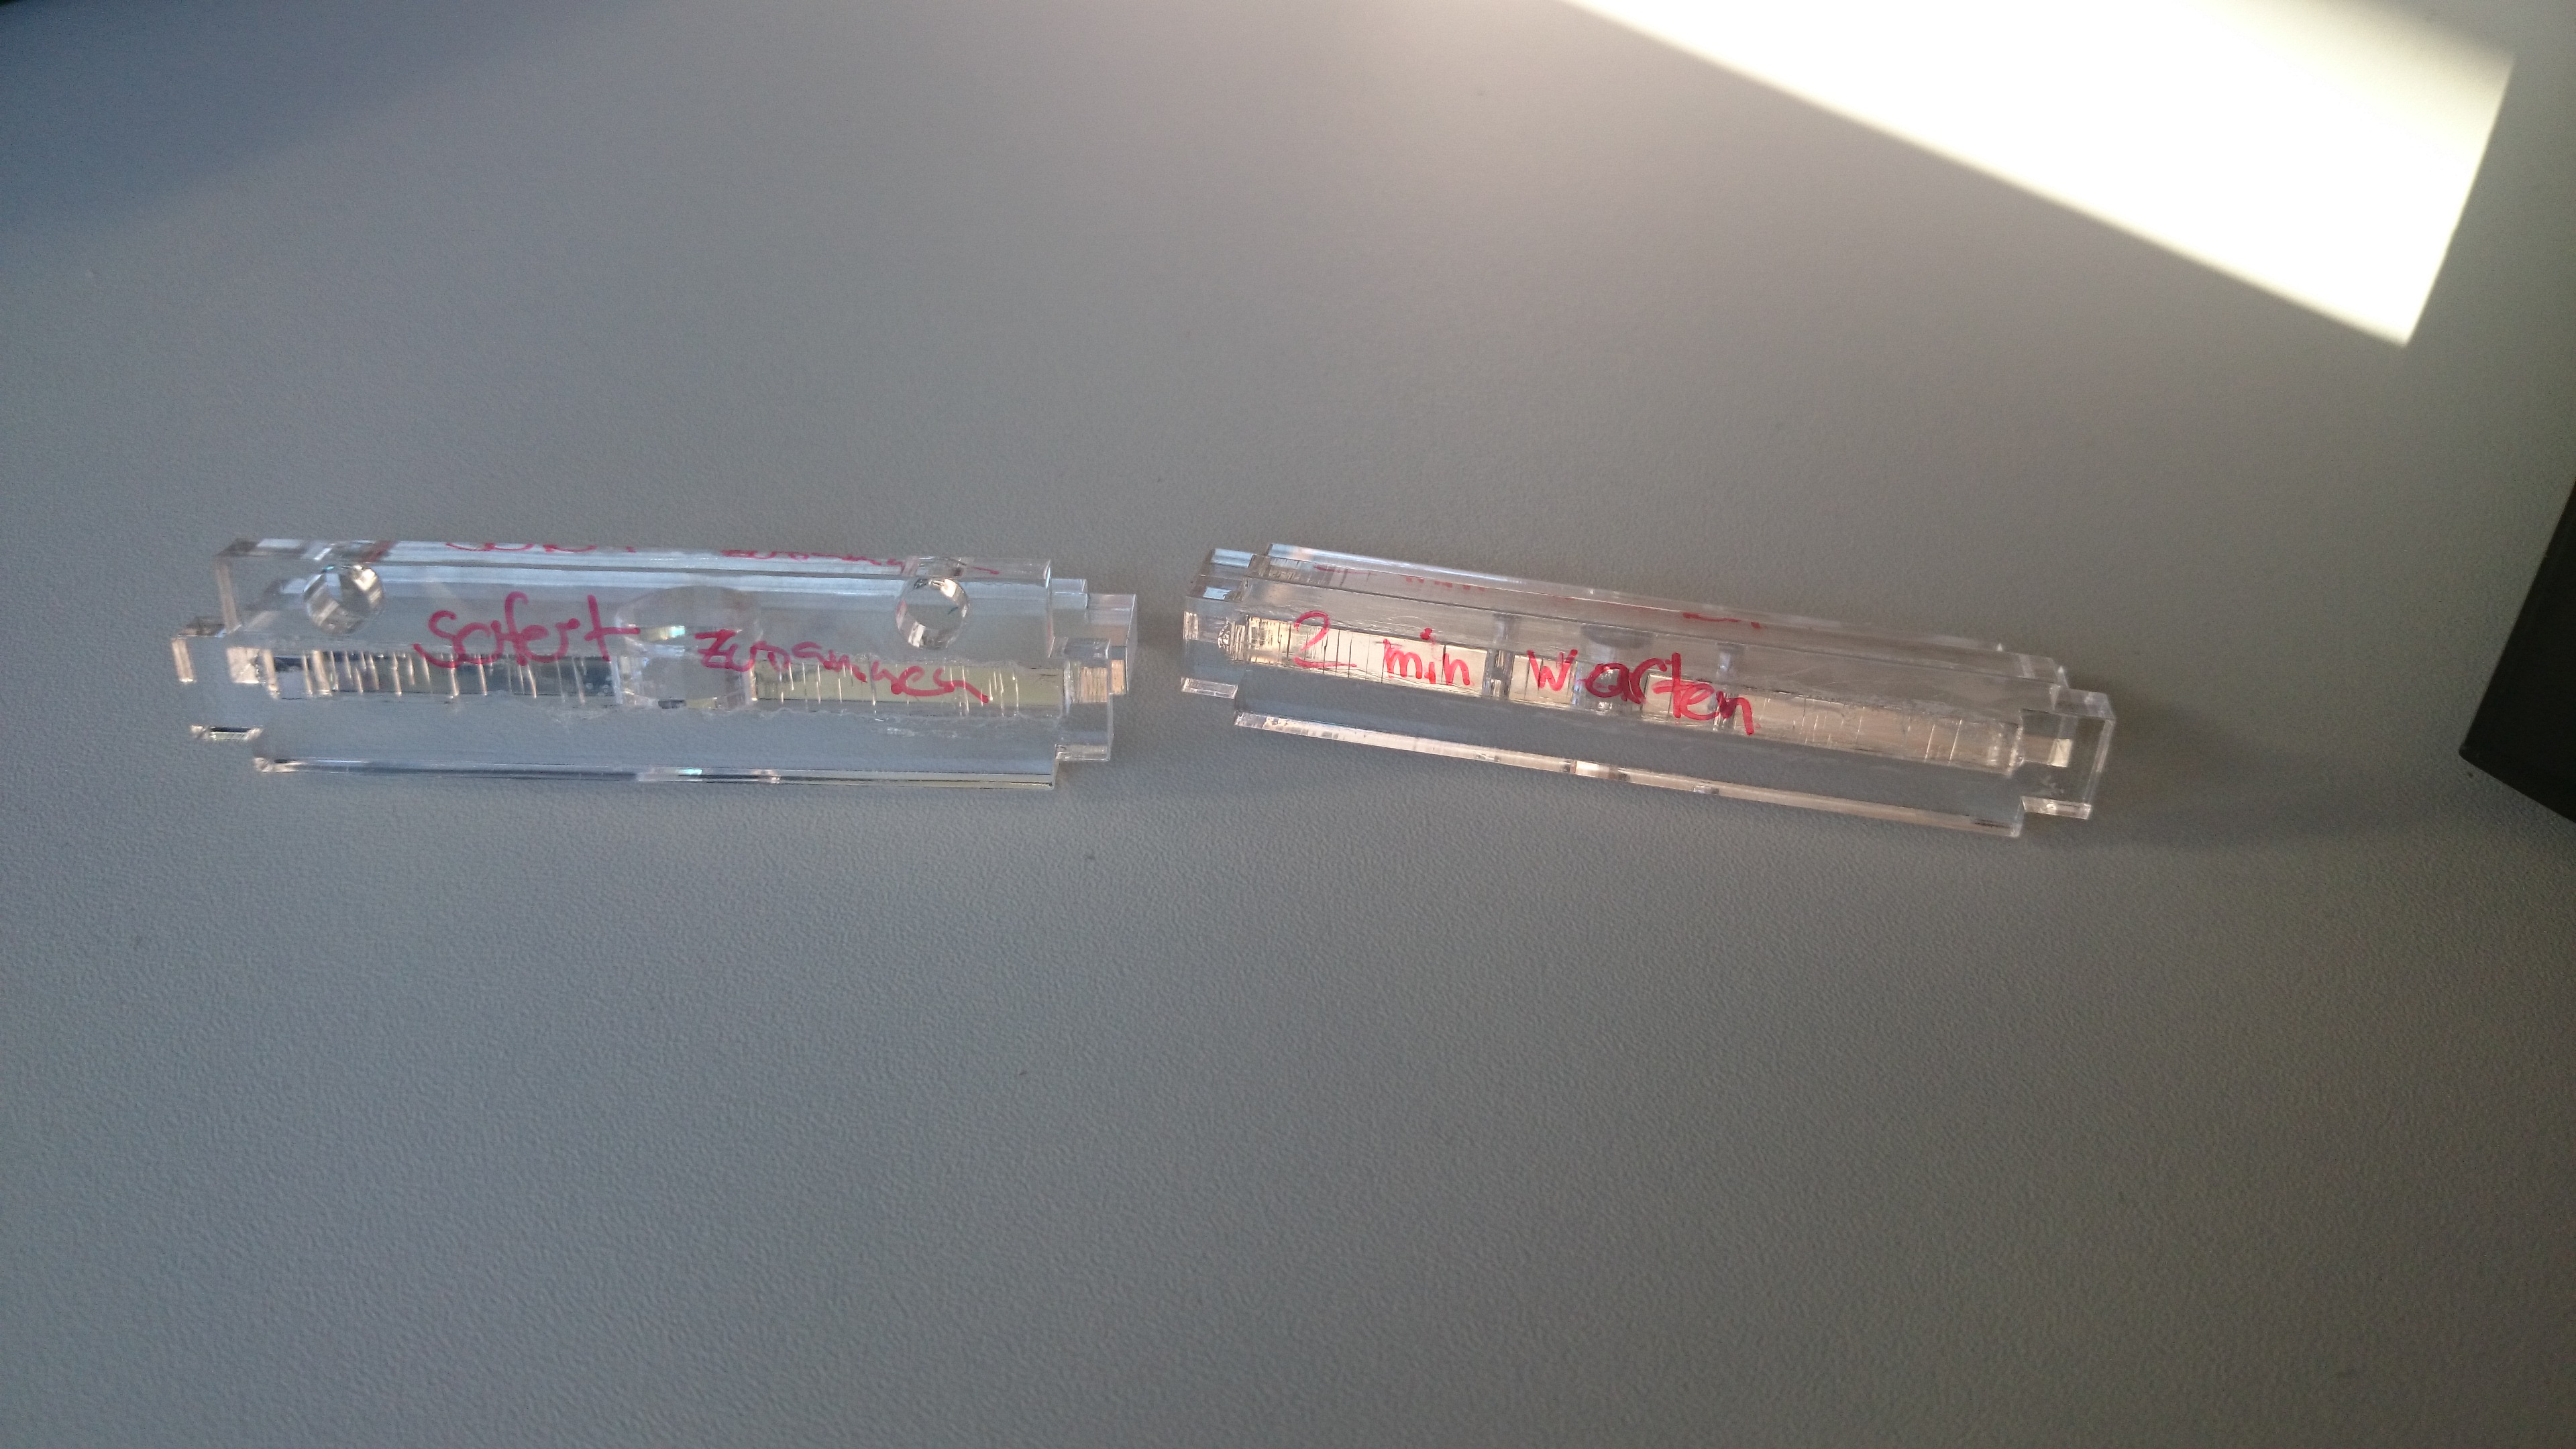
\includegraphics[width=0.7\textwidth,clip,trim=0cm 0cm 0cm 0cm]
	{Testberichte/Klebeversuch.jpg}
	\centering
	\caption{Klebeversuch mit UHU Kleber} 
	\label{abb:Klebeversuch}
\end{figure}
    
\subsection{Führungsschaufel}
\begin{tabular}{p{3.6cm}p{\textwidth-3.6cm-0.7cm}}
	\rule{0pt}{11pt}\textit{Typ}              & Führungsschaufel\\
	\rule{0pt}{11pt}\textit{Datum}:           & 13.03.2015   \\
	\rule{0pt}{11pt}\textit{Ort}:             & Werkstatt \\
	\rule{0pt}{11pt}\textit{Tester}:          & Pascal Roth und Matteo Trachsel  \\
	\rule{0pt}{11pt}\textit{Ziel des Testes}: & Das Ziel des Testes besteht darin, verschieden Führungsschaufeln zu testen und eine geeignete Befestigung zu finden. \\
	
	
	\rule{0pt}{11pt}\textit{Aufbau / Ablauf}: &
	Für den Test wurden aus einem 1 mm dicken Aluminiumblech, welches bereits auf die Breite des Förderbandes zugeschnitten wurde, verschieden Lange Stücke abgeschnitten. Da pro Tennisball zwei Führungsschaufeln vorne und hinten benötigt werden, gibt es zwei Möglichkeiten zur Gestaltung der Führungsschaufeln. Die erste Möglichkeit besteht darin, dass immer eine einzelne Schaufel für je vorne und hinten realisiert wird. Die zweite Möglichkeit besteht darin, dass man die hinter und die nächste vorne liegende Führungschaufel zusammen in einem Blechstück realisiert.\\
	
	
	\rule{0pt}{11pt}\textit{Fazit / Verbesserungs-\newline vorschlag}: &
	Durch den Versuch stellte sich heraus, dass es sich besser eignet, wenn zwei Führungsschaufeln zusammen in einem Blechstück realisiert werden. Wenn die Führungschaufelpaare mit dem UHU Kleber am vorderen Rand angeklebt werden, können sie immer noch den Radius der Wellen überfahren, ohne sich abzulösen. Zur Sicherheit können die Führungsschaufeln noch mit einem Klebeband befestigt werden. \\
\end{tabular}

\begin{figure}[h!]
	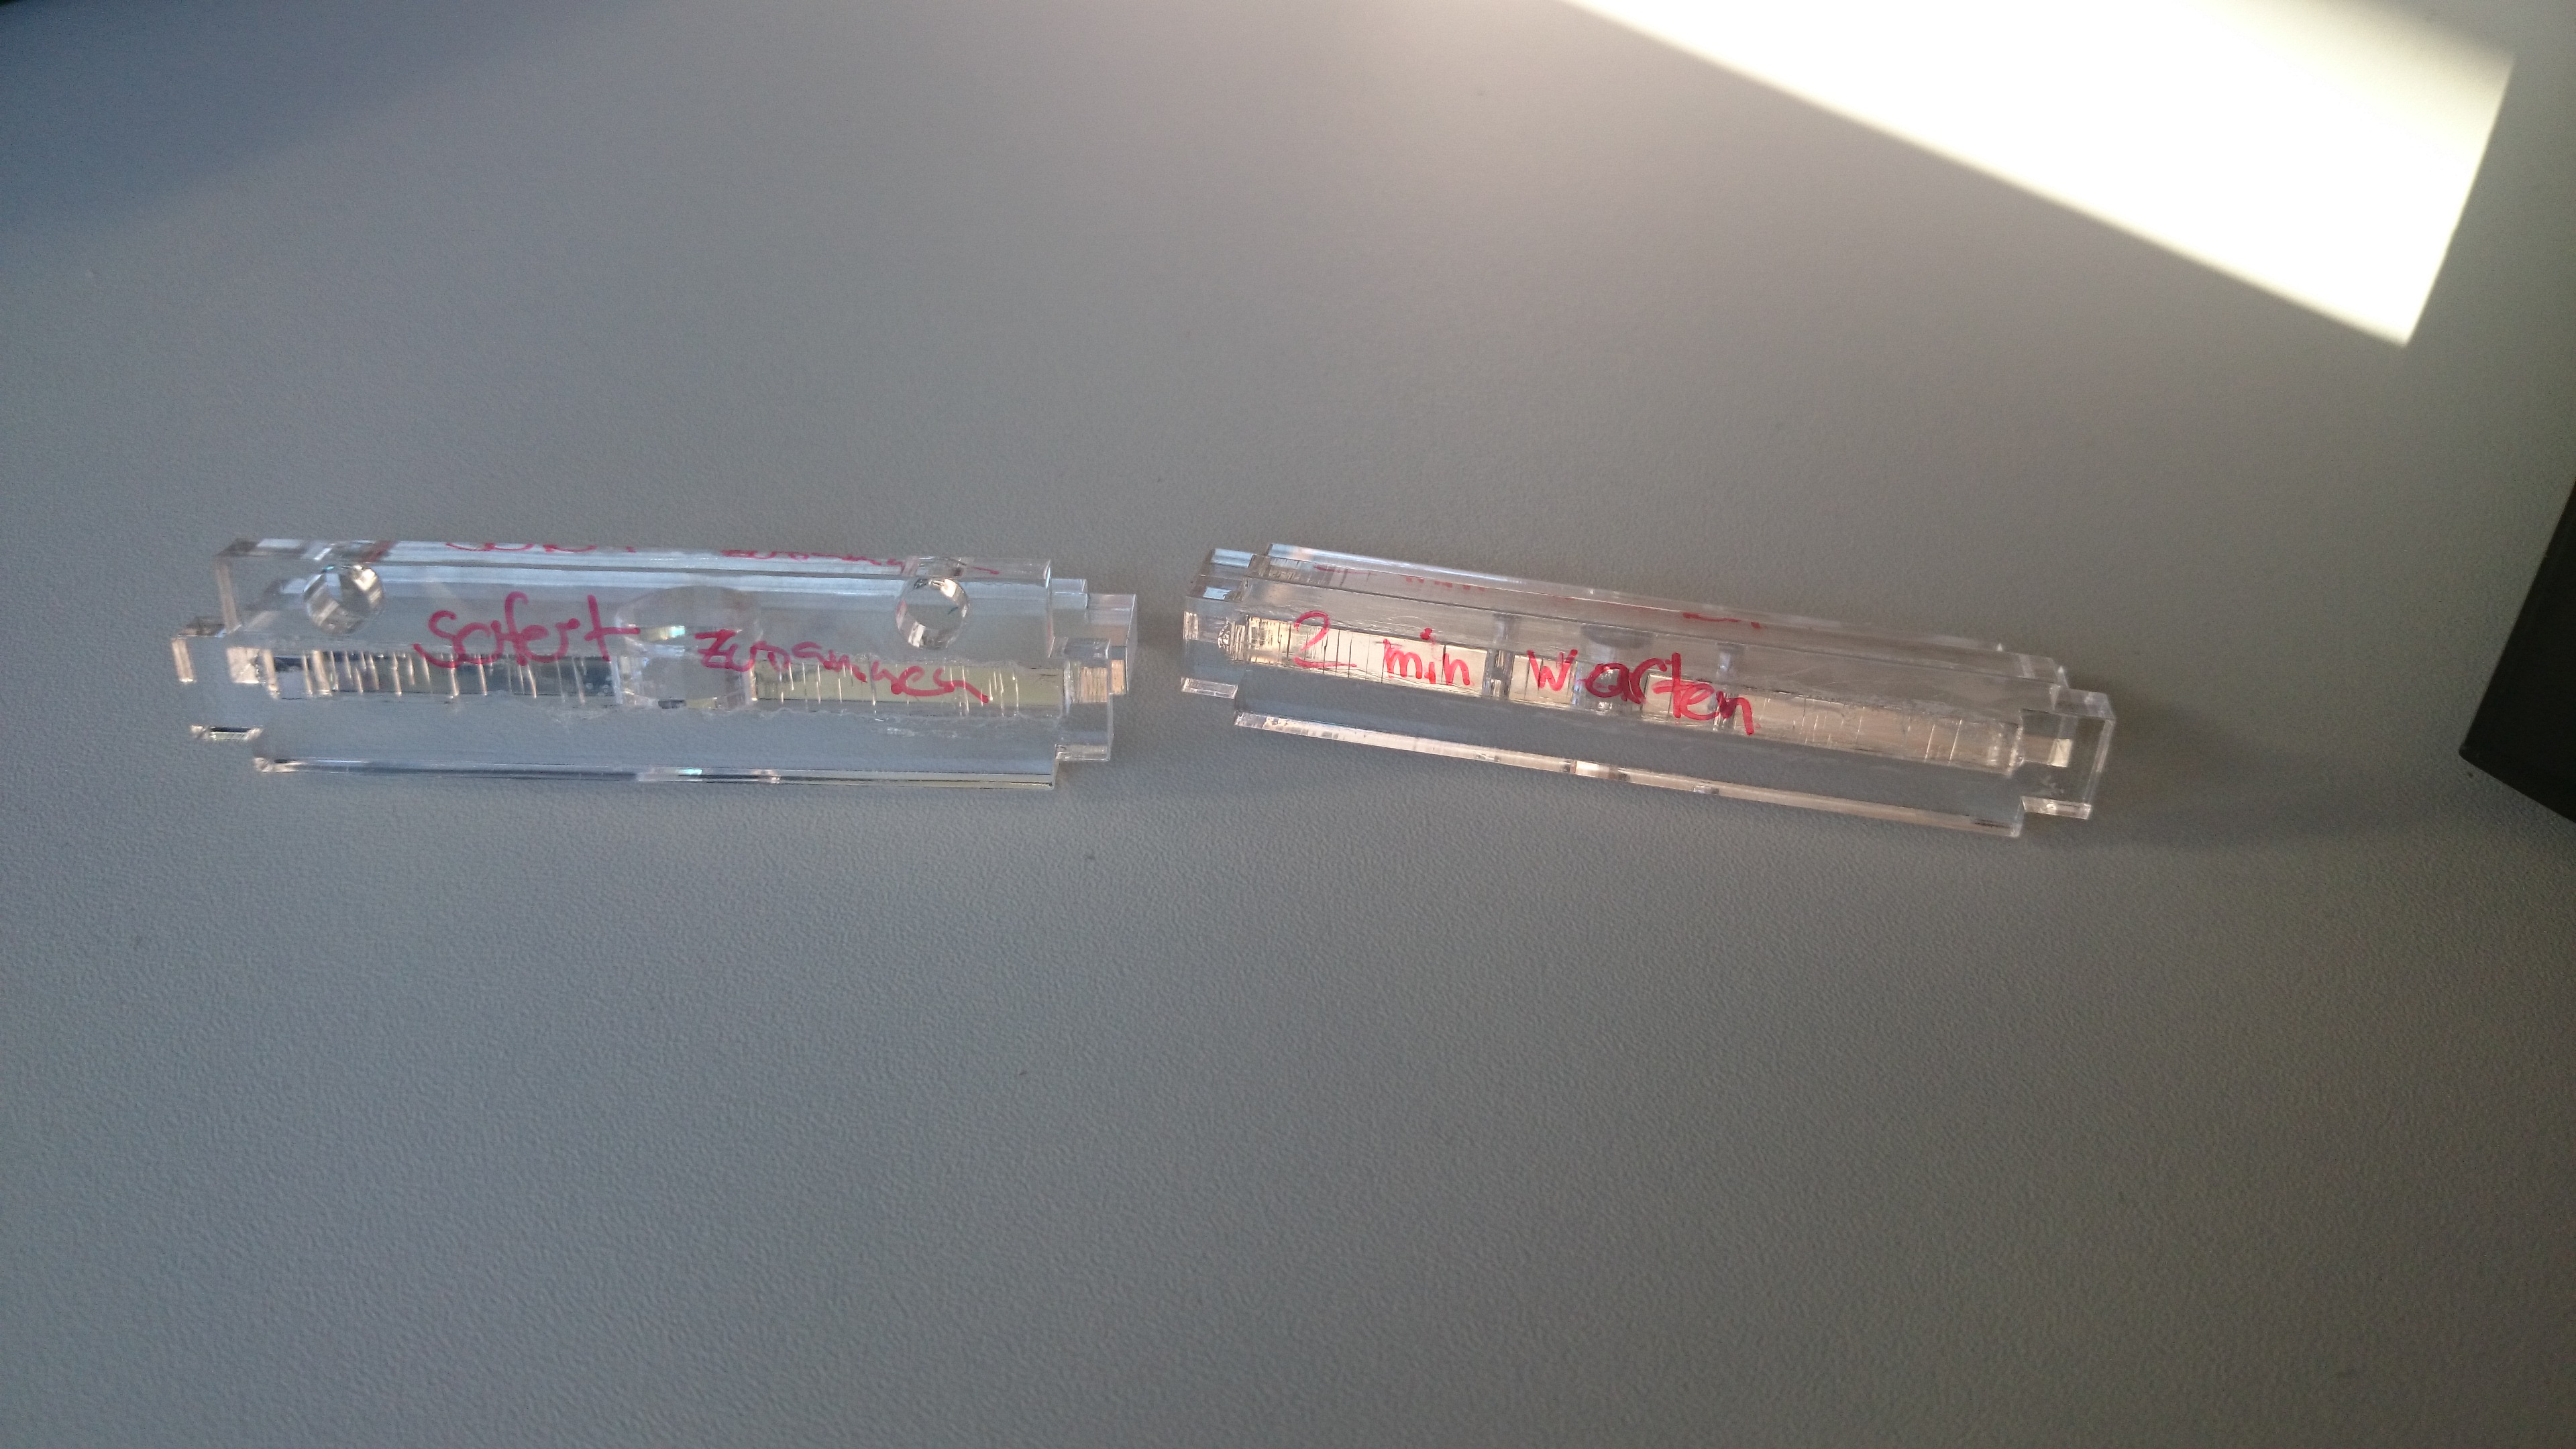
\includegraphics[width=0.9\textwidth,clip,trim=10cm 15cm 40cm 6cm]
	{Testberichte/Klebeversuch.jpg}
	\centering
	\caption{Förderband mit Führungschaufeln}
	\label{abb:Klebeversuch}
\end{figure}



    \section{Förderband}
\label{sec:Foerderband}
	Da die Beschleunigungsräder durch den Abwurf abgebremst werden, müssen 
	sie nach jedem Wurf wieder auf Nenndrehzahl gebracht werden. Um dafür 
	genügend Zeit zu haben, erfolgt die Zuführung der Bälle in zeitlichen 
	Abständen. Ein weiteres Kriterium für eine konstante Wurfweite, ist eine 
	gleichbleibende Geschwindigkeit mit der die Bälle zwischen die 
	Beschleunigungsräder kommen. Der Antrieb des Förderbandes erfolgt mit 
	einem DC-Motor, siehe Kapitel \ref{sec:FoerderbandAnsteuerung}. Die 
	Drehzahl ist mittels einer Zahnradpaarung mit $i=5$ übersetzt, um das 
	benötigte Drehmoment an die Antriebswelle des Förderbandes zu übertragen. 
	Die Antriebswelle und die Achse sind einteilig aus Aluminium gedreht. 
	Welle und Achse sind mittels Kugellager in den Seitenplatten gelagert. 
	Die Auflagefläche des Riemens auf der Antriebswelle ist bombiert gefertigt. 
	Dadurch wird ein seitliches Abrutschen des Riemens im Betrieb verhindert. 
	Auf dem Förderband, welches ein Flachbandriemen ist, sind Führungsschaufeln 
	angebracht, siehe Abbildung \ref{abb:Foerderband}. Durch den Abstand dieser 
	Schaufeln, ergeben sich die kurzen 
	Pausen um die Motoren hochzudrehen. Die Führungsschaufeln sind so 
	ausgerundet, dass der Ball möglichst lange geführt werden kann ohne die 
	Beschleunigungsräder zu berühren. Die Schaufeln sind aus $1\si{\milli\meter}$ 
	Aluminium Blech gefertigt und wurden auf dem Riemen aufgeklebt. Bei den 
	Testversuchen stellte sich heraus, dass durch die aufgeklebten Schaufeln 
	der Riemen nicht rund läuft. Jedes Mal wenn eine Klebestelle die Achse 
	passierte, erhöhte sich der Widerstand und das Band drehte langsamer. 
	Ausserdem hat der Endlosriemen an der Stelle an der er gefügt ist eine 
	höhere Steifigkeit, was denselben Effekt hatte. Ausgehend von diesen 
	Erkenntnissen wurde der Riemen neu gefertigt. Die Schaufeln wurden nicht 
	mehr geklebt, sondern mit einem Faden angenäht. Dazu wurden in Riemen 
	und Führungsschaufeln je drei Bohrungen gemacht und mit verstärktem Faden 
	Verbunden. So sind die Führungsschaufeln nur noch mit einer Linienverbindung 
	und nicht mehr mit einer Flächenverbindung auf dem Riemen befestigt. An 
	der Fügestelle des Riemens wurde in Längsrichtung Material entnommen, was 
	eine Verringerung der Steifigkeit bewirken sollte. In den nachfolgenden 
	Testversuchen zeigten die Anpassungen ihre gewünschte Wirkung. Die 
	Geschwindigkeit während einer Umdrehung war nun annähernd konstant. Aus 
	diversen Testversuchen der Ballzuführung während PREN1 wurde erkannt, dass 
	für einen idealen Abwurf die Tennisbälle mit beiden Beschleunigungsräder 
	gleichzeitig in Kontakt kommen müssen. Somit ist es notwendig die Bälle 
	zunächst unter dem oberen Beschleunigungsrad hindurch und anschliessend in 
	einem 45\si{\degree} Winkel nach oben zuzuführen. Dazu dient ein Führungselement, 
	siehe Abbildung \ref{abb:Abschusswinkel}
	welches auf beiden Seiten des Acrylglases angebracht ist. Diese 
	Führungselemente sind an die Form der Tennisbälle angepasst und mittels 
	3D Druck hergestellt worden. 
	\begin{figure}[h!]
    	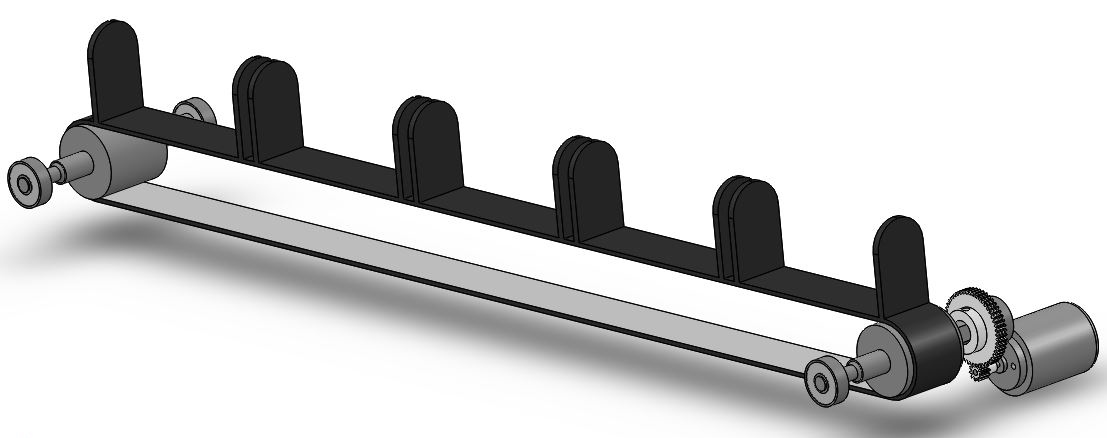
\includegraphics[width=0.9\textwidth,clip,trim=0mm 0mm 0mm 0mm]
    	{Enddokumentation/Bilder/Foerderband.jpg}
    	\centering
    	\caption{Aufbau des Förderbandes}
    	\label{abb:Foerderband}
 	\end{figure}

\subsection{Ansteuerung DC-Motor}
\label{sec:FoerderbandAnsteuerung}
    Die Ansteuerung des Motors, der das Förderband antreibt, erfolgt mittels PWM. Auf diese 
    Weise lässt sich die Drehzahl und somit die Nachführgeschwindigkeit einstellen. Das 
    Band muss nur in eine Richtung angetrieben werden, wodurch die Ansteuerung einfacher 
    realisiert werden kann. Das Schema ist in Abbildung \ref{abb:SchemaAnsteuerung} 
    ersichtlich. Im wesentlichen besteht diese Ansteuerung aus einem Vortreiber und einem 
    Schalter. Der Treiber bewirkt ein möglichst schnelles und effizientes Öffnen und Schliessen des Schalters. Auf diese Weise reduziert man die Schaltverluste. 
    \begin{figure}[h!]
    	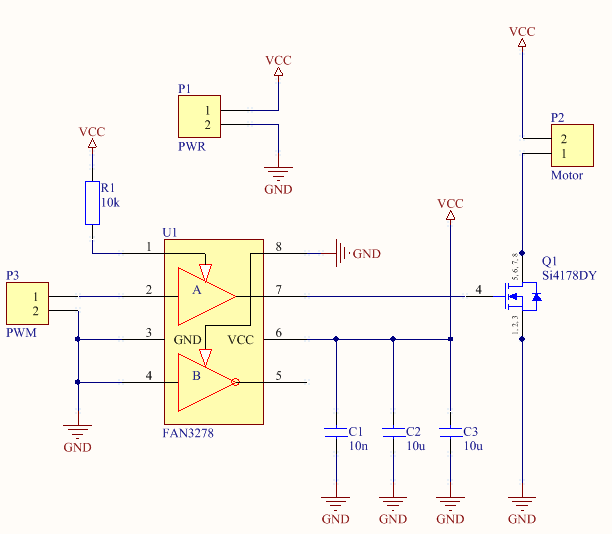
\includegraphics[width=0.7\textwidth,clip,trim=0mm 2mm 0mm 7mm]
    	{Enddokumentation/Bilder/Schema_DC-Ansteuerung.png}
    	\centering
    	\caption{Schema des Förderbandansteuerung}
    	\label{abb:SchemaAnsteuerung}
    \end{figure}
    \subsection{Bildaufnahme mit Smartphone inklusive persistente Speicherung}
\begin{zebratabular}{p{4.5cm}p{\textwidth-3.6cm-0.7cm}}
    \rule{0pt}{11pt}\textit{Tester}              & Thomas Wiss \\ 
    \rule{0pt}{11pt}\textit{Datum}:           & 26.03.2015   \\
    \rule{0pt}{11pt}\textit{Ort}:             & Teaminsel \\
    \rule{0pt}{11pt}\textit{Beschreibung}:          & Mittels dem aufgenommenen Bild wird ein 
    Schwarz/Weiss-Abgleich erstellt und der PREN-Korb erkennt. Das Bild wird aufgenommen und 
    anschliessend in einem internen Verzeichnis des Smartphones abgespeichert. 
    Es handelt sich hier um einen Komponententest. \\
    \rule{0pt}{11pt}\textit{Akteure}:          & Operator zur Bedienung des Android-Phones. \\
    \rule{0pt}{11pt}\textit{Bedingung}:          & Lauffähiges Android-Phone mit 
    Android-Applikation \enquote{CameraSD}. \\
    \rule{0pt}{11pt}\textit{Erwartete Fehlermeldung}:          & keine \\
    \rule{0pt}{11pt}\textit{Vorgehen}:          & Applikation öffnen und Button \enquote{Take Picture}
     betätigen. Mittels Android-Explorer den Speicherort des Bildes verifizieren. \\
    \rule{0pt}{11pt}\textit{Erwartetes Ergebnis}:          & Gespeichertes Bild, am 
    vorgängig programmierten Speicherort. \\
    \rule{0pt}{11pt}\textit{Eingetretenes Ergebnis}:          & Bild in guter Qualität am 
    programmierten Speicherort gespeichert. \\
    \rule{0pt}{11pt}\textit{Test bestanden?}:          & Ja \\
    \rule{0pt}{11pt}\textit{Weiter Tests nötig?}:          & Nein \\
\end{zebratabular}    


    \subsection{Förderband Ballzuführung}
\begin{zebratabular}{p{4.5cm}p{\textwidth-3.6cm-0.7cm}}
    \rule{0pt}{11pt}\textit{Tester}           & Matteo Trachsel\\ 
    \rule{0pt}{11pt}\textit{Datum}:           & 26.03.2015   \\
    \rule{0pt}{11pt}\textit{Beschreibung}:    & Um die Bälle möglichst schnell zu den Beschleunigungsräder zu fördern, muss das Förderband gleichmässig, zentral und ohne Schlupf auf der Welle laufen. \\
    \rule{0pt}{11pt}\textit{Akteure}:         & Welle mit DC-Motor für Antrieb und Stirnrädern, Förderriemen mit aufgeklebten Leitschaufeln, Achse mit Spannelement. \\
    \rule{0pt}{11pt}\textit{Bedingung}:       & Funktionsmuster soweit montiert dass Förderreimen betrieben werden kann.\\
    \rule{0pt}{11pt}\textit{Erwartete Fehlermeldung}:          & keine \\
    \rule{0pt}{11pt}\textit{Vorgehen}:        & Förderreimen einsetzen, spannen, mit fünf Bällen bestücken. Spannung an DC-Motor anlegen. \\
    \rule{0pt}{11pt}\textit{Erwartetes Ergebnis}: & Bälle werden nach vorne befördert. Förderreimen bleibt mittig auf Achse und Welle (??***wort vergessen). Kein Schlupf zwischen Welle und Riemen. \\
    \rule{0pt}{11pt}\textit{Eingetretenes Ergebnis}: & Funktionsfähigkeit bestätigt. Erkenntnis: Schlupf auf Welle ist kein Problem. Je weniger der Riemen gespannt ist, desto gleichmässiger ist der Lauf. Keine Gefahr des seitlichen Ablaufens des Riemens. \newline
    Negativ: Durch ungenaue Bearbeitung läuft Stirnrad nicht Rund. 
    \\
    \rule{0pt}{11pt}\textit{Test bestanden?}:     & Ja, allerdings neues Stirnrad bestellen und nochmals bearbeiten.  \\
    \rule{0pt}{11pt}\textit{Weiter Tests nötig?}: & Nein \\
\end{zebratabular}  
    \subsection{Windelverstellung}
\begin{zebratabular}{p{4.5cm}p{\textwidth-5.3cm}}
    \rule{0pt}{11pt}\textit{Tester}           & Roger Gisler\\ 
    \rule{0pt}{11pt}\textit{Datum}:           & 17.04.2015\\
    \rule{0pt}{11pt}\textit{Beschreibung}:    & Um den Ballwerfer zum Korb hin auszurichten, ist eine Verstelleinheit montiert. Diese verändert den Winkel des Ballwerfers gegenüber seiner Anfangsposition bis auf einen gewünschten Wert. \\
    \rule{0pt}{11pt}\textit{Akteure}:         & Schrittmotor mit Ritzel welches in den Zahnkranz am Ende der Grundplatte eingreift.\\
    \rule{0pt}{11pt}\textit{Bedingung}:       & Funktionsmuster soweit montierte. Bälle auf Förderband. Mit zusätzlichen Gewichten belastet um Endgewicht von zu simulieren. \\
    \rule{0pt}{11pt}\textit{Erwartete Fehlermeldung}:          & keine \\
    \rule{0pt}{11pt}\textit{Vorgehen}:        & Schrittmotor ansteuern, und in beide Drehrichtungen drehen. Ineinandergreifen der Verzahnung, ruckfreier Lauf, Festigkeit der Bauteile überprüfen. \\
    \rule{0pt}{11pt}\textit{Erwartetes Ergebnis}: & Ruckfreier Lauf, optimaler Eingriff der Verzahnung über den gesamten Verstellwinkel gewährleistet. Verstellung in beide Richtungen. \\
    \rule{0pt}{11pt}\textit{Eingetretenes Ergebnis}: & Ritzel und Zahnrad greifen über den gesamten Verstellwinkel optimal ineinander. Kraft des Schrittmotor ausreichend. 
    Festigkeit des Ritzels aus Acrylglas nicht ausreichend, was zum Bruch des Bauteils führte. 
    Stabilität des gesamten Ballwerfers kritisch da sich ein grosser Teil des Gewichts auf dem vorderen Drehpunkt befindet. \\
    \rule{0pt}{11pt}\textit{Test bestanden?}:     & Nein \\
    \rule{0pt}{11pt}\textit{Weiter Tests nötig?}: & Ja \\
    \rule{0pt}{11pt}\textit{Weiteres Vorgehen}: & Ritzel aus MDF (höhere Elastizität) Lasern.
    Vorderer Quersteg(Acrylglas) auf dem ein grosser Teil des Gewichts lastet aus Aluminium fertigen um die Durchbiegung und Schwingungen zu eliminieren. 
    Grundplatte im vorderen Bereich rund um den Drehpunkt neu Konstruieren um die Kippgefahr zu eliminieren und die Seitliche Stabilität zu erhöhen. \\
\end{zebratabular}  
    \subsection{Zahnradgetriebe der Beschleunigungsräder}
\begin{zebratabular}{p{4.5cm}p{\textwidth-3.6cm-0.7cm}}
    \rule{0pt}{11pt}\textit{Tester}           & Pascal Roth\\ 
    \rule{0pt}{11pt}\textit{Datum}:           & 09.04.2015\\
    \rule{0pt}{11pt}\textit{Beschreibung}:    & Um die Kraft der Motoren auf die Beschleunigungsräder zu übertragen, muss Eingriff und Wellenabstand der Zahnräder stimmen.\\
    \rule{0pt}{11pt}\textit{Akteure}:         & Je zwei Zahnradpaarungen pro Beschleunigungsrad.\\
    \rule{0pt}{11pt}\textit{Bedingung}:       & Achsen, Wellen und Zahnräder des Getriebes montiert, Achsabstand auf variabler Seite eingestellt. Motoren montiert (nicht angeschlossen)\\
    \rule{0pt}{11pt}\textit{Erwartete Fehlermeldung}:          & keine \\
    \rule{0pt}{11pt}\textit{Vorgehen}:        & Motor manuell drehen. Eingriff, Rundlauf, axiale Verschiebung der Zahnräder überprüfen. \\
    \rule{0pt}{11pt}\textit{Erwartetes Ergebnis}: & Eingriff, Achsabstand, Rundlauf stimmen analog CAD Modell\\
    \rule{0pt}{11pt}\textit{Eingetretenes Ergebnis}: & Alles IO.\\
    \rule{0pt}{11pt}\textit{Test bestanden?}:     & Ja \\
    \rule{0pt}{11pt}\textit{Weiteres Vorgehen}: & Test mit erhöhter Drehzahl\\
\end{zebratabular}  
    \subsection{Zahnradgetriebe der Beschleunigungsräder II}
\begin{zebratabular}{p{4.5cm}p{\textwidth-3.6cm-0.7cm}}
    \rule{0pt}{11pt}\textit{Tester}           & Pascal Roth / Yves Studer\\ 
    \rule{0pt}{11pt}\textit{Datum}:           & 16.04.2015\\
    \rule{0pt}{11pt}\textit{Beschreibung}:    & Erweiterung des ersten Zahnradgetriebe Tests. Antrieb durch Motoren mit Nenndrehzahl.\\
    \rule{0pt}{11pt}\textit{Akteure}:         & Je zwei Zahnradpaarungen pro Beschleunigungsrad. Brushless-Motoren inkl. deren Ansteuerung.\\
    \rule{0pt}{11pt}\textit{Bedingung}:       & Achsen, Wellen und Zahnräder des Getriebes montiert, Achsabstand auf variabler Seite eingestellt. Motoren montiert, angeschlossen und funktionsfähig.\\
    \rule{0pt}{11pt}\textit{Erwartete Fehlermeldung}:          & keine \\
    \rule{0pt}{11pt}\textit{Vorgehen}:        & Motoren auf Nenndrehzahl beschleunigen. Verhalten des Getriebes bezüglich Schwingungen und Vibrationen überprüfen. Festigkeit der Welle-Nabe Verbingdungen.\\
    \rule{0pt}{11pt}\textit{Erwartetes Ergebnis}: & Verhalten des ersten Testlaufs auch mit höherer Drehzahl bestätigt. \\
    \rule{0pt}{11pt}\textit{Eingetretenes Ergebnis}: & Eingriff der Verzahnung auch mit hohen Drehzahlen okay. Keine übermässigen Vibrationen. Welle-Nabe Verbindung Zahnrad – Welle der Beschleunigungsräder ist dem Beschleunigungsmoment nicht gewachsen. Achse aus Gleitlagermaterial iglidur ist der Thermischen Belastung durch die Reibung nicht gewachsen.
    \\
    \rule{0pt}{11pt}\textit{Test bestanden?}:     & Verzahnung Ja\newline
    Lagerung Nein\newline
    Welle-Nabe Nein\\
    \rule{0pt}{11pt}\textit{Weiteres Tests nötig}: & Ja\\
    \rule{0pt}{11pt}\textit{Weiteres Vorgehen}: & Defekte Achse aus Aluminium fertigen. Phase in Welle der Beschleunigungsräder Fräsen damit Stellschraube mehr Halt findet. \\
\end{zebratabular}  
    \subsection{Zahnradgetriebe der Beschleunigungsräder III}
\begin{zebratabular}{p{4.5cm}p{\textwidth-3.6cm-0.7cm}}
    \rule{0pt}{11pt}\textit{Tester}           & Pascal Roth / Yves Studer\\ 
    \rule{0pt}{11pt}\textit{Datum}:           & 23.04.2015\\
    \rule{0pt}{11pt}\textit{Beschreibung}:    & Wiederholung des Tests Zahnradgetriebe II mit neuer Achse und optimierter Welle-Nabe Verbindung. \\
    \rule{0pt}{11pt}\textit{Akteure}:         & Je zwei Zahnradpaarungen pro Beschleunigungsrad. Brushless-Motoren inkl. deren Ansteuerung. Speziell Achse des Getriebes und Welle-Nabe Verbindung zwischen der Welle der Beschleunigungsräder und dessen Zahnrad.\\
    \rule{0pt}{11pt}\textit{Bedingung}:       & Achsen, Wellen und Zahnräder des Getriebes montiert, Achsabstand auf variabler Seite eingestellt. Motoren montiert, angeschlossen und funktionsfähig.\\
    \rule{0pt}{11pt}\textit{Erwartete Fehlermeldung}:          & keine \\
    \rule{0pt}{11pt}\textit{Vorgehen}:        & Motoren auf Nenndrehzahl beschleunigen. Sitz der erwähnten Welle-Nabe Verbindung unter verschiedenen Betriebsbedingungen und Lastwechsel. Verhalten der Gleitlagerpaarung Alu-achse Kunststoffzahnrad.\\
    \rule{0pt}{11pt}\textit{Erwartetes Ergebnis}: & Bauteile sind nun den erhöhten Belastungen gewachsen. \\
    \rule{0pt}{11pt}\textit{Eingetretenes Ergebnis}: & Welle-Nabe Verbindung auch nach mehreren Beschleunigungszyklen und Lastwechsel noch fest. Neue Achse aus Aluminium ist der Belastung gewachsen. 
    \\
    \rule{0pt}{11pt}\textit{Test bestanden?}:     & Ja\\
    \rule{0pt}{11pt}\textit{Weiteres Vorgehen}: & Nein\\
\end{zebratabular}  
    \clearpage
    \subsection{Kommunikation zwischen Freedom-Board und Android-Phone}
\begin{tabular}{p{4.5cm}p{\textwidth-3.6cm-0.7cm}}
    \rule{0pt}{11pt}\textit{Tester}              & Thomas Wiss \\ 
    \rule{0pt}{11pt}\textit{Datum}:           & 16.04.2015   \\
    \rule{0pt}{11pt}\textit{Ort}:             & Teaminsel \\
    \rule{0pt}{11pt}\textit{Beschreibung}:          & Um den auf dem Android-Phone berechneten 
    Winkel zum Freedom-Board zu senden, muss die Kommunikation zwischen dem Freedom-Board 
    und dem Android-Phone getestet werden. \\
    \rule{0pt}{11pt}\textit{Akteure}:          & Operator zur Bedienung des Android-Phones. \\
    \rule{0pt}{11pt}\textit{Bedingung}:          & USB-Kabel muss am Android-Phone und gleichzeitig 
    auch am Freedom-Board eingesteckt sein. \\
    \rule{0pt}{11pt}\textit{Erwartete Fehlermeldung}:          & keine \\
    \rule{0pt}{11pt}\textit{Vorgehen}:          & USB-Kabel am Android-Phone und am 
    Freedom-Board einstecken. Starten der Applikation \enquote{SerialPortExample} auf dem Android-Phone. 
    Den Befehl \enquote{debug} ins Textfeld eintragen und den Button Send betätigen. \\
    \rule{0pt}{11pt}\textit{Erwartetes Ergebnis}:          & Die Rückmeldung in der TextBox 
    muss ein Informations- und Hilfemenu anzeigen. \\
    \rule{0pt}{11pt}\textit{Eingetretenes Ergebnis}:          & Siehe Abbildung 
    \ref{abb:ScreenshotSerialPortExampleTestProtokol}. \\
    \rule{0pt}{11pt}\textit{Test bestanden?}:          & Ja \\
    \rule{0pt}{11pt}\textit{Weiter Tests nötig?}:          & Nein \\
\end{tabular}    
    \newline
    \newline
    \begin{figure}[h!]
    	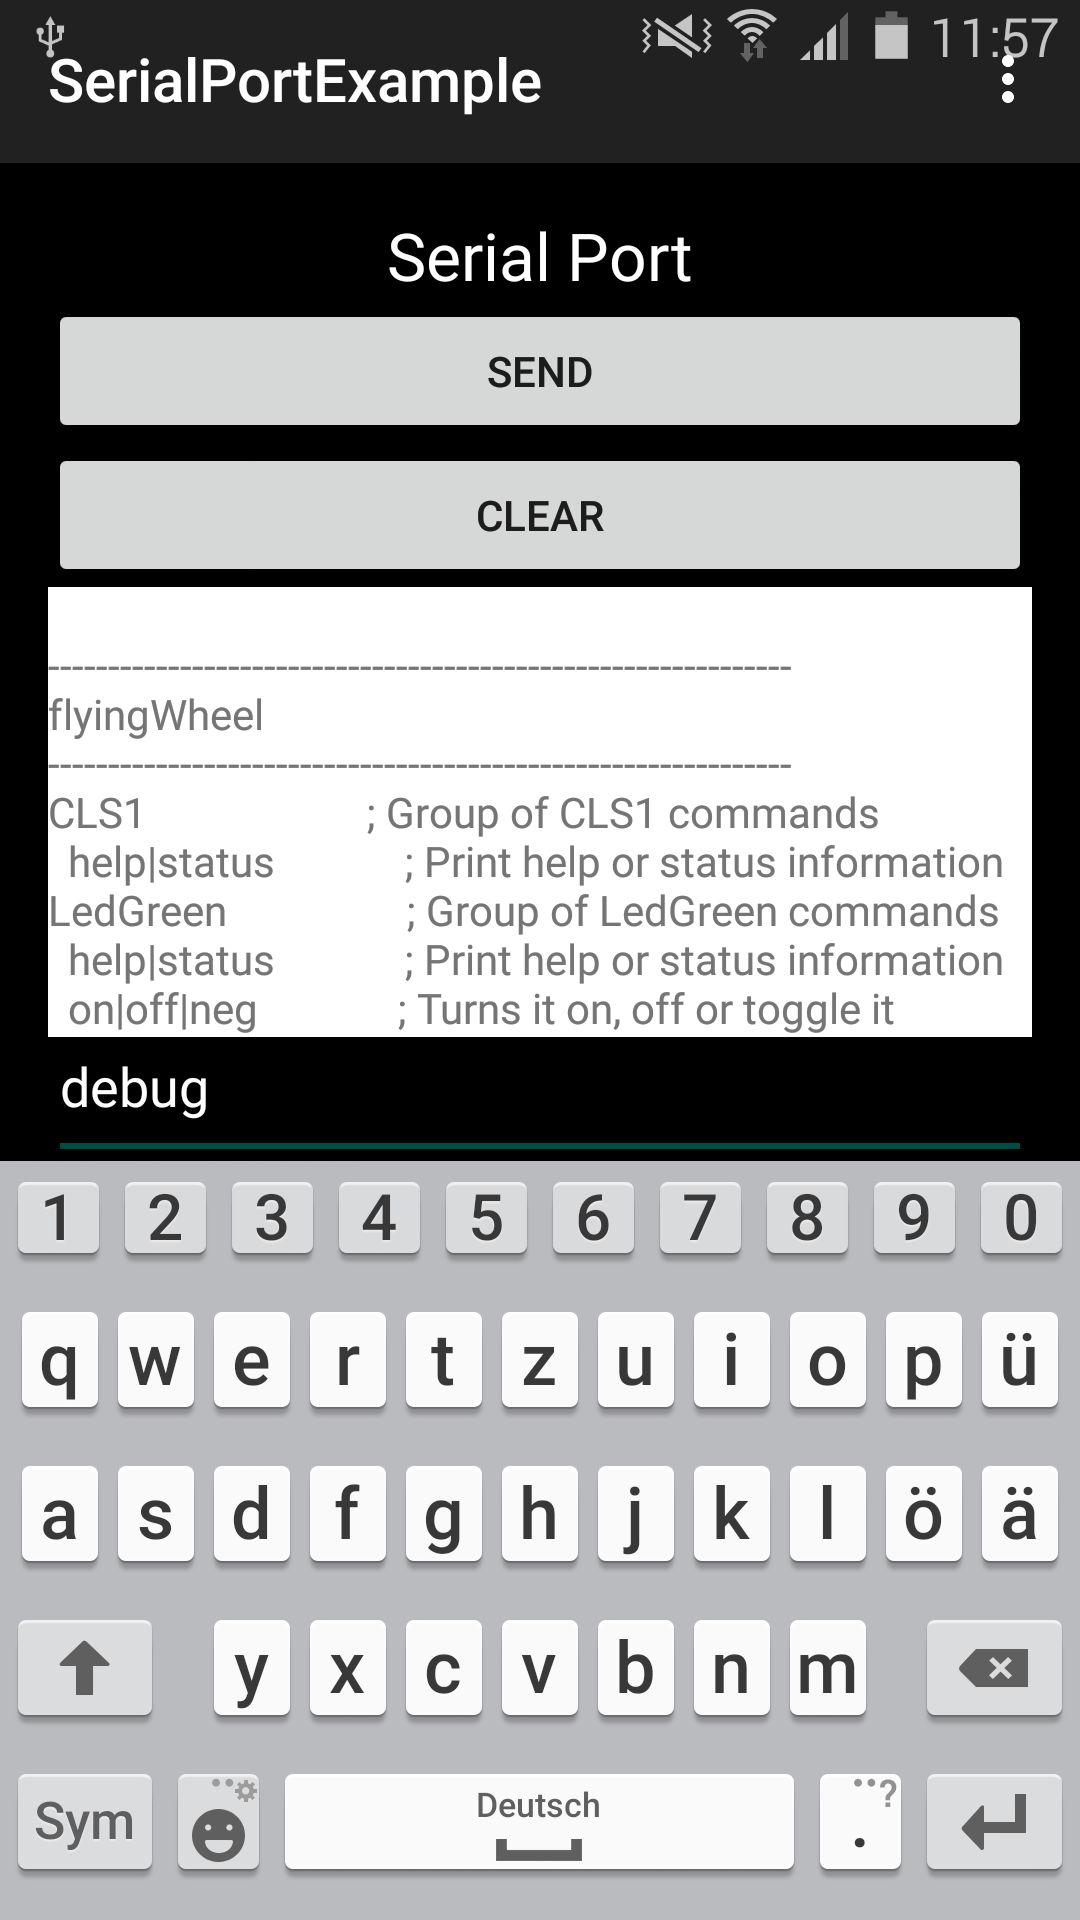
\includegraphics[width=0.3\textwidth,clip,trim=0mm 0mm 0mm 0mm]
    	{Enddokumentation/Bilder/Screenshot_SerialPortExample_debug.png}
    	\centering
    	\caption{Screenshot der Applikation \enquote{SerialPortExample}}
    	\label{abb:ScreenshotSerialPortExampleTestProtokol}
    \end{figure}
    

    \clearpage
    % Testprotkolle Informatik als PDF's
    \newpage
    
    
    % % % %
    \begin{flushleft}
        \setlength\bibitemsep{2\itemsep}
        %\nocite{*} %Alle Quellen ausgeben
        \renewcommand{\refname}{Literatur- und Quellenverzeichnis}
%        \{\refname}{Quellenverzeichnis}
        \bibliography{Enddokumentation/ET-Gruppe/et-gruppe_source,../common/Quellen}{} %!!! Kein Leerzeichen nach dem , !!!!
    \end{flushleft}
    %
    % Beginn des Anhangs
    %
    \appendix      
   	\begin{appendix}
   		\clearpage
   		\pagenumbering{Roman} % römische Nummerierung des Anhangs (Grosse Buchstaben)
   		\section{Anhang}
   		
   		
   		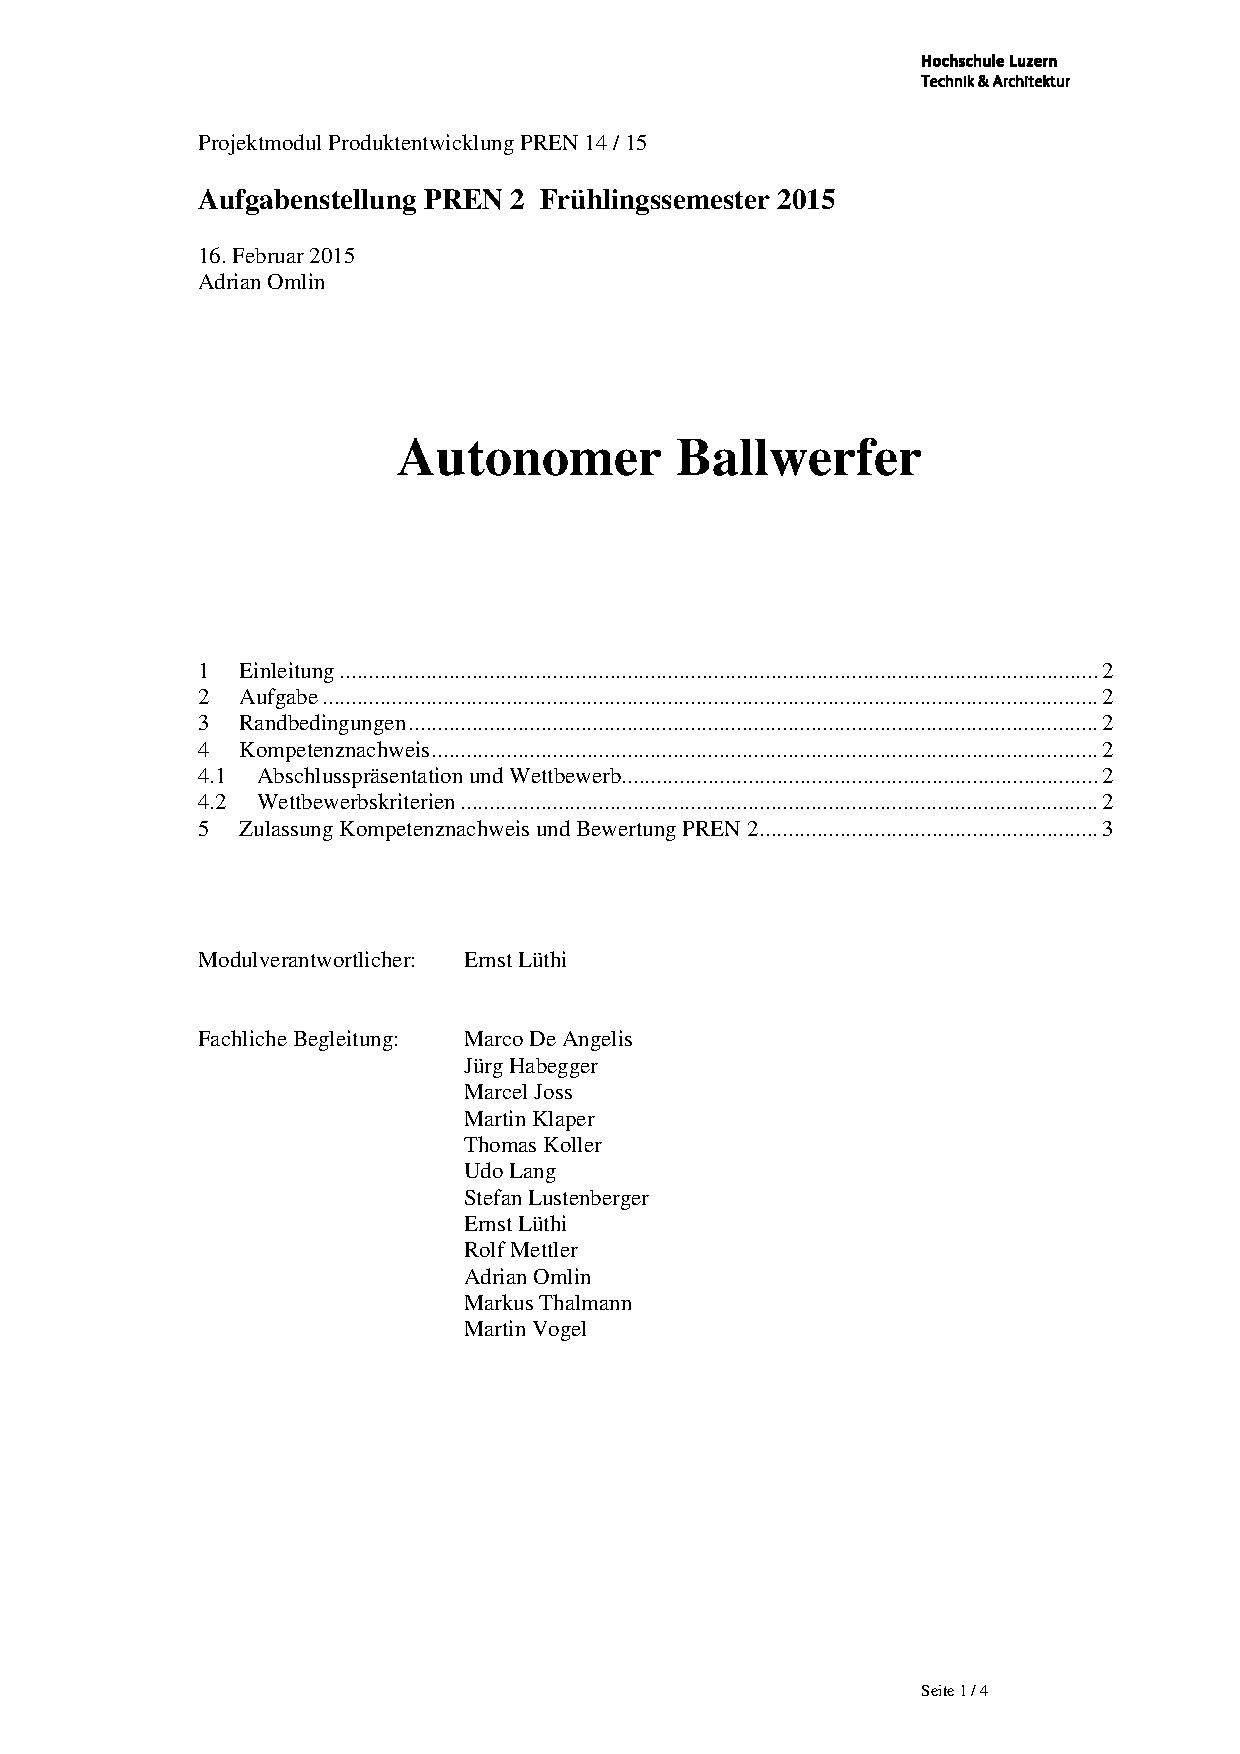
\includepdf[page=1 , offset=0cm -1.9cm, width=1.05\textwidth,picturecommand={\centering},pagecommand=\section{Aufgabenstellung PREN 2}{\thispagestyle{fancy}},]{Anhang/Aufgabenstellung_PREN2_F15.pdf}
   		
   		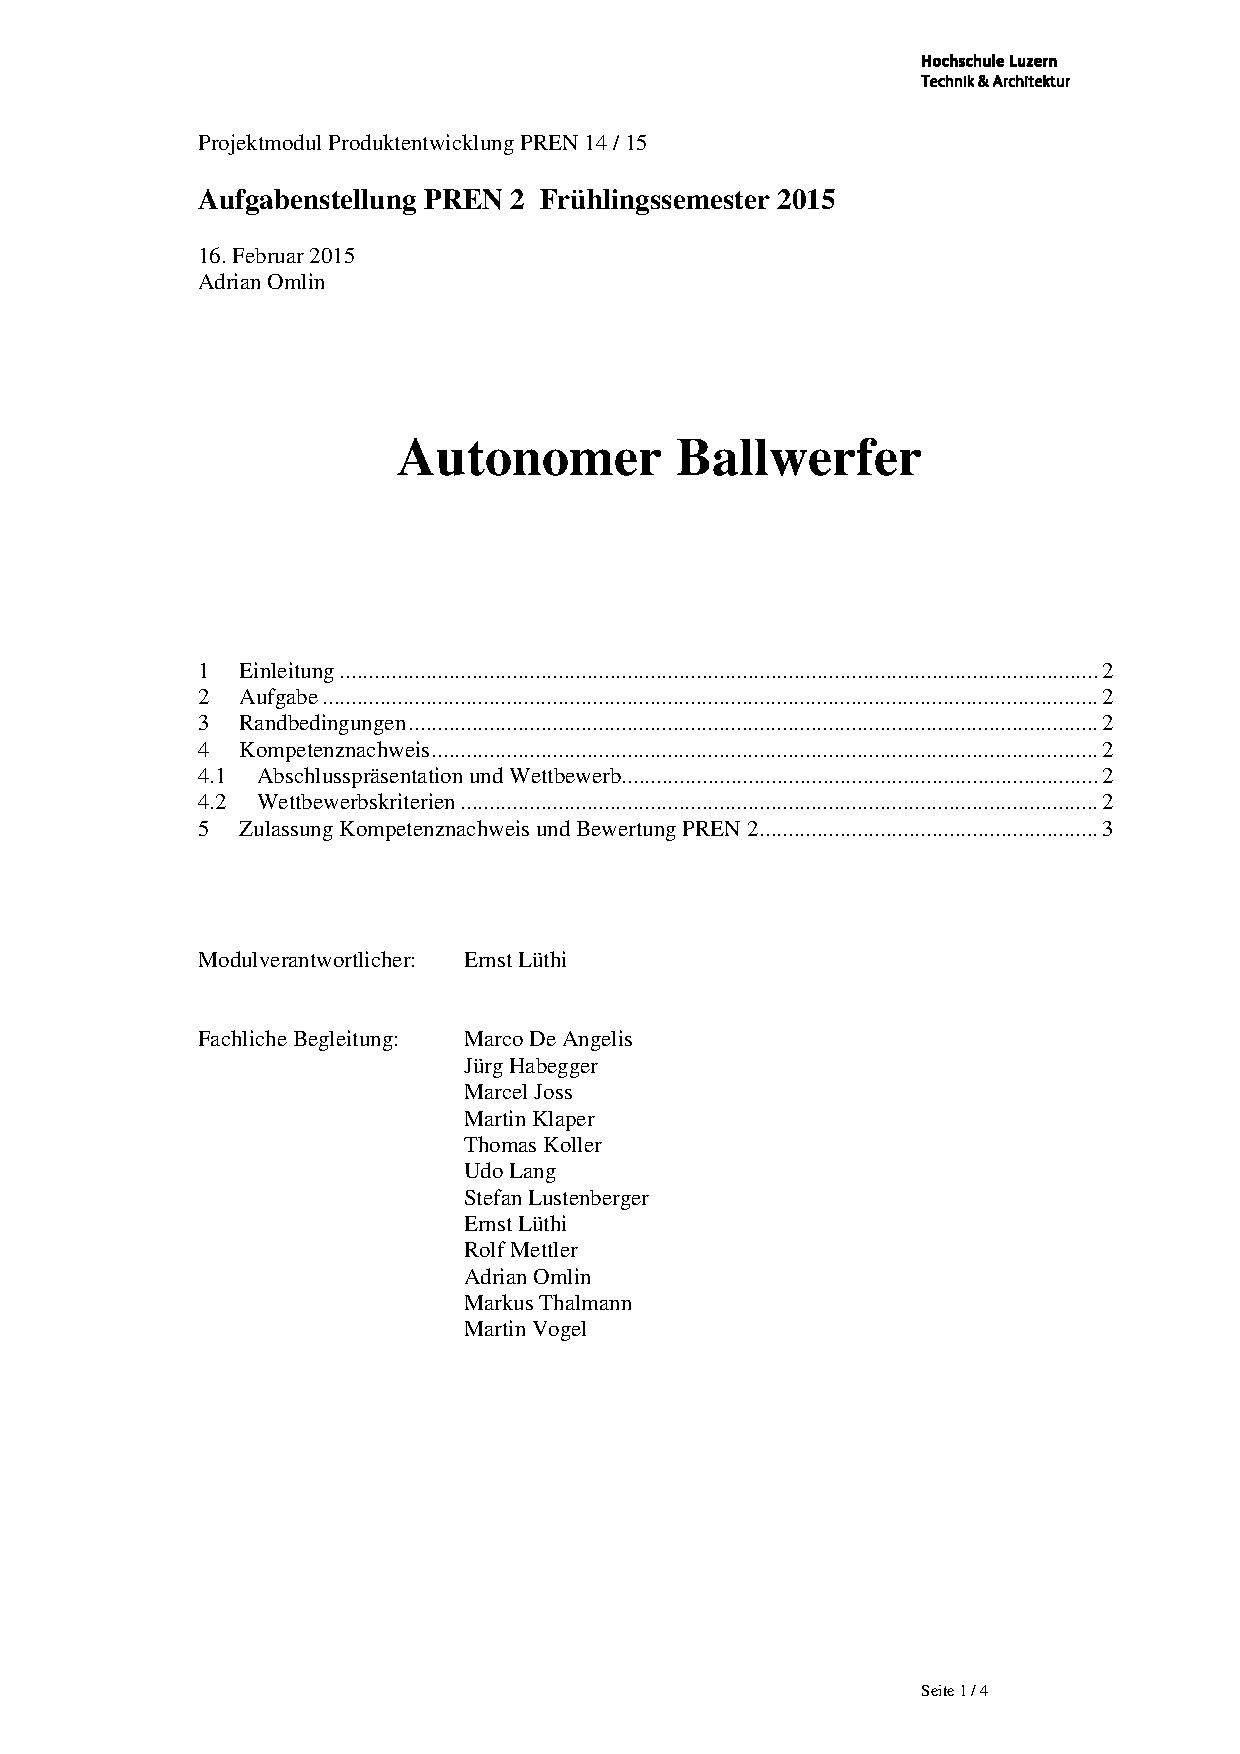
\includepdf[page=2- , offset=0cm -1.60cm, width=1.1\textwidth,picturecommand={\centering},pagecommand={\thispagestyle{fancy}},]{Anhang/Aufgabenstellung_PREN2_F15.pdf}
   		
   		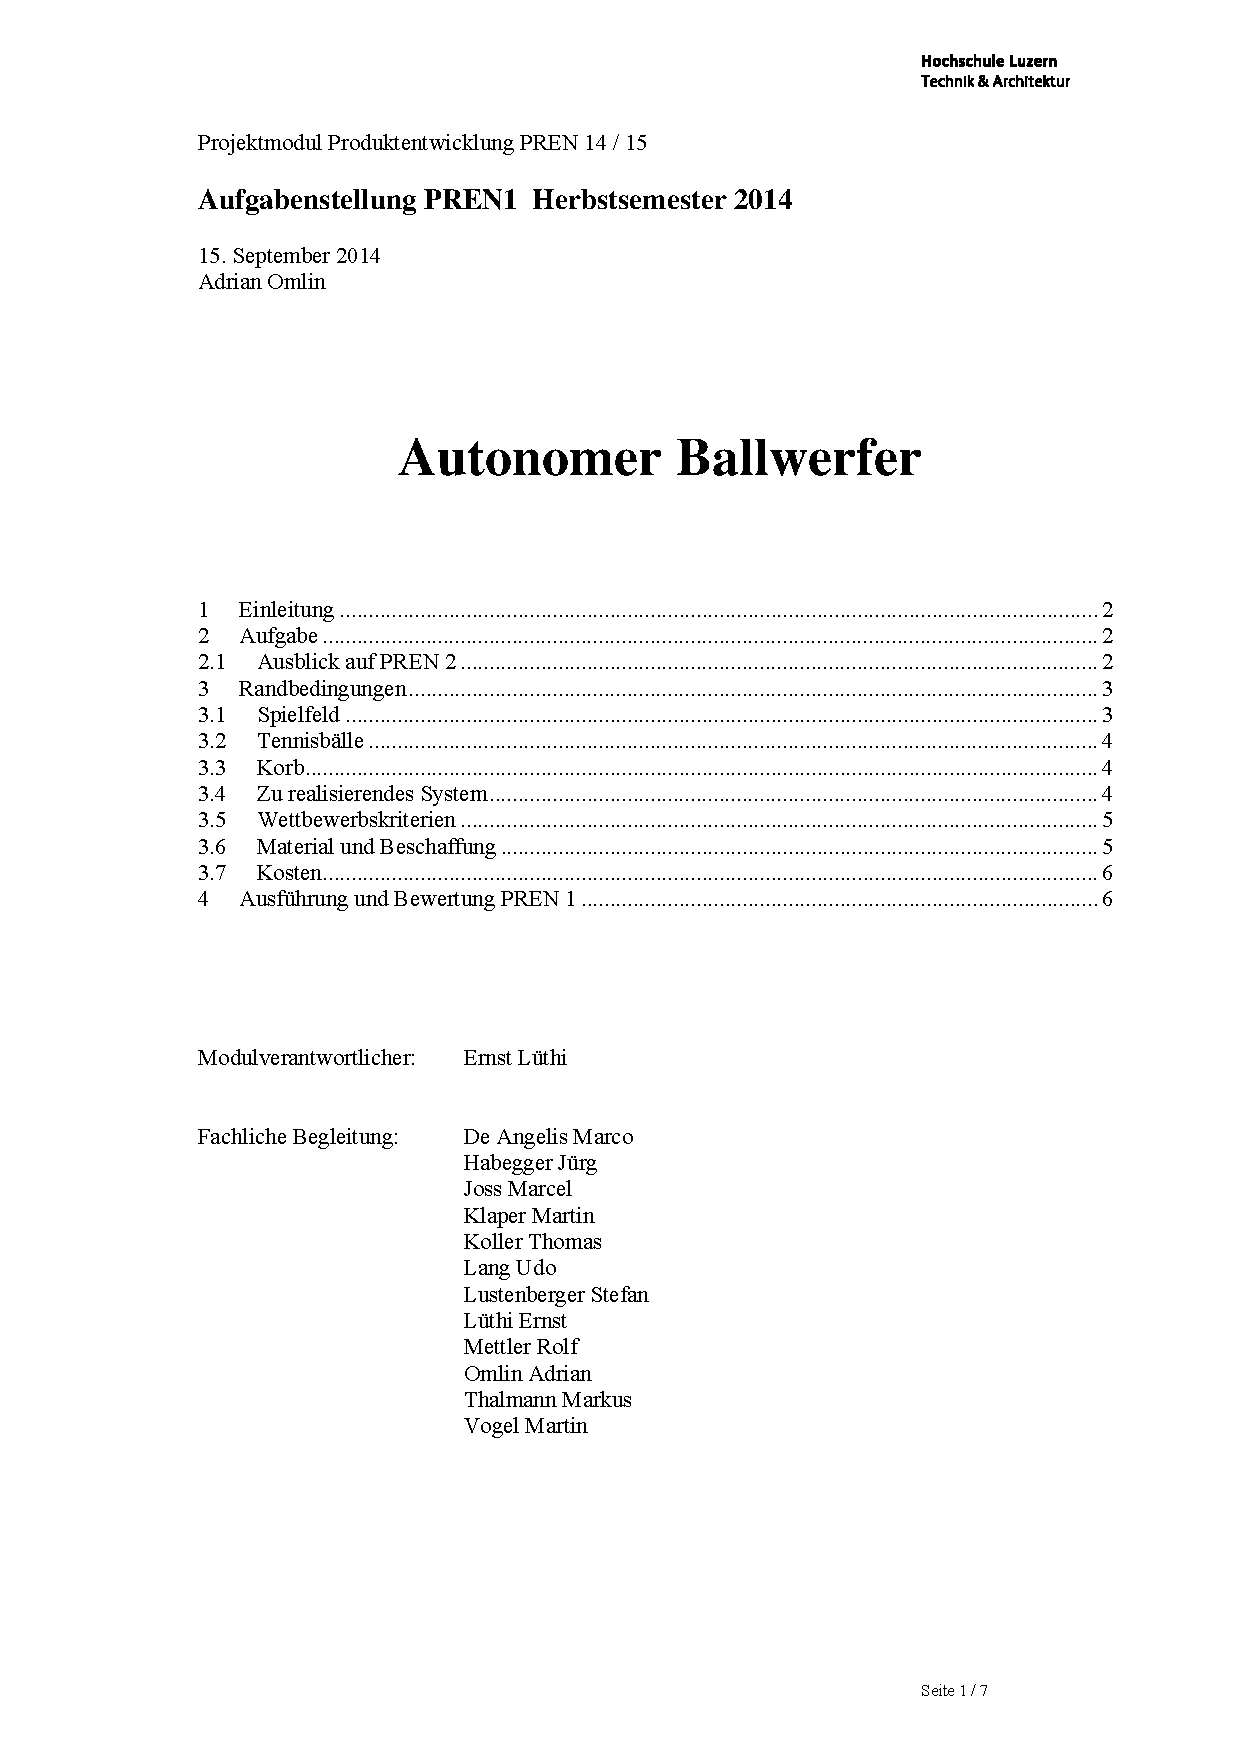
\includepdf[page=1 , offset=0cm -1.9cm, width=1.05\textwidth,picturecommand={\centering},pagecommand=\section{Aufgabenstellung PREN 1}{\thispagestyle{fancy}},]{Anhang/Aufgabenstellung_PREN1_H14.pdf}
   			
   		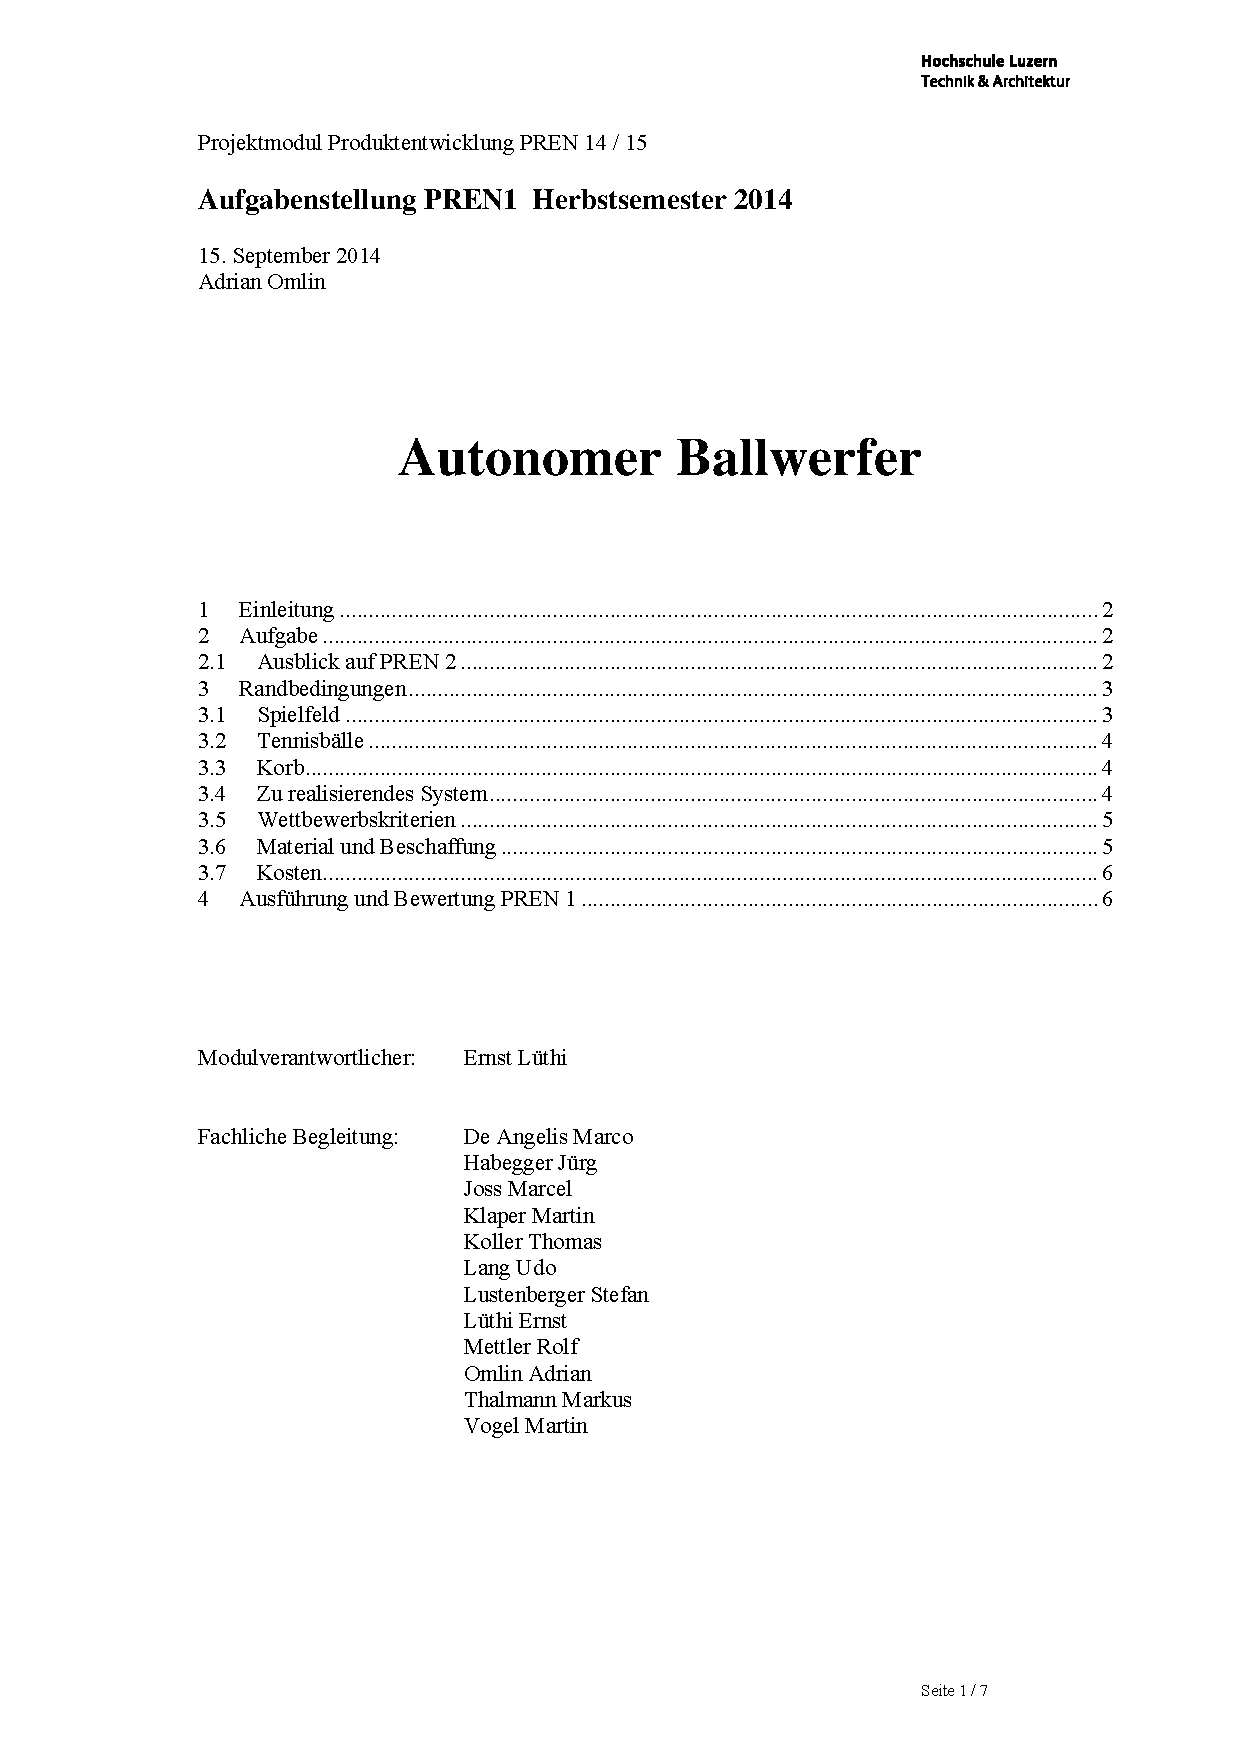
\includepdf[page=2- , offset=0cm -1.60cm, width=1.1\textwidth,picturecommand={\centering},pagecommand={\thispagestyle{fancy}},]{Anhang/Aufgabenstellung_PREN1_H14.pdf}
   		
   		\begin{landscape}
   			\section{Risikokatalog}
   			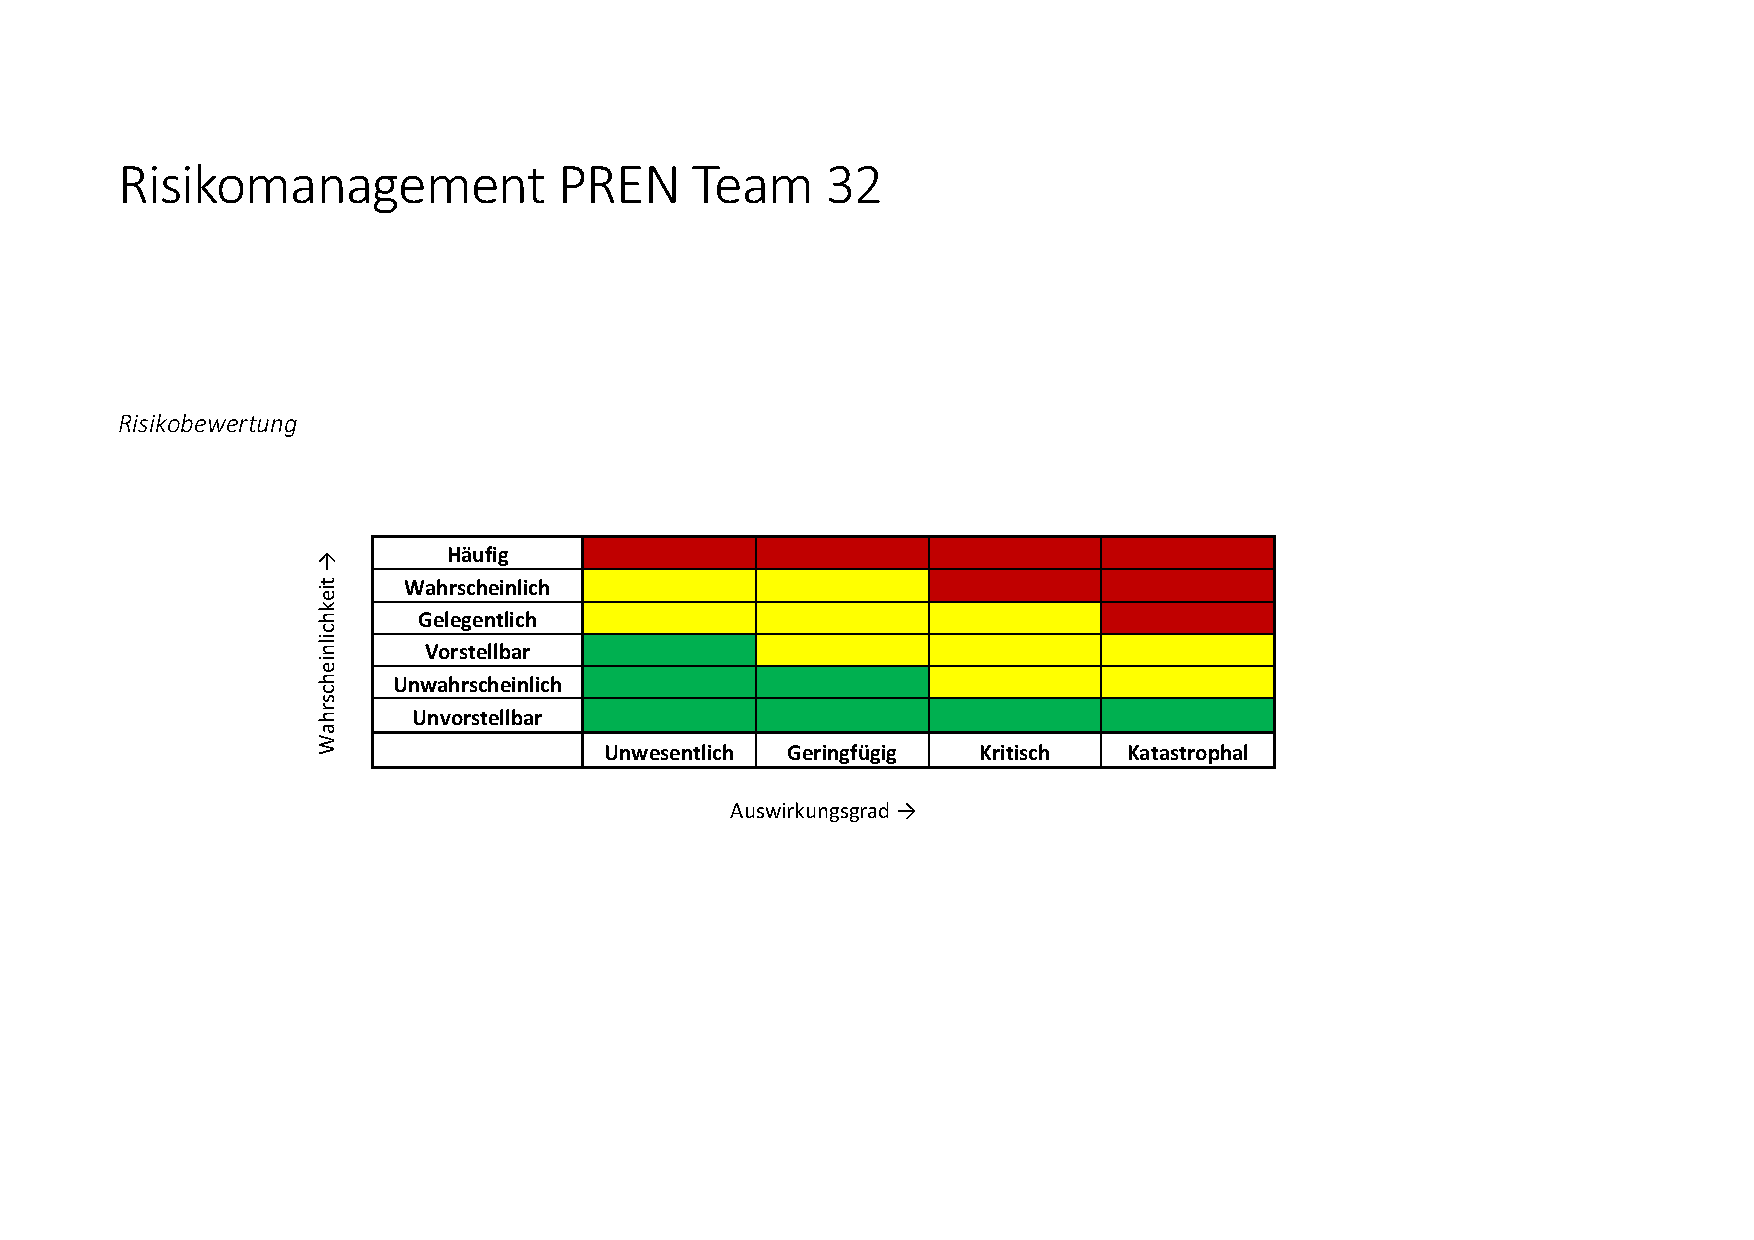
\includegraphics[page=1,scale=0.73,clip,trim=17mm 27mm 31mm 39mm]{Anhang/Risikomanagement.pdf}
   			\newpage  			
   			\includegraphics[page=2,scale=1,clip,trim=20mm 22mm 21mm 32mm]{Anhang/Risikomanagement.pdf}
   			\newpage  			
   			\includegraphics[page=3,scale=1,clip,trim=20mm 22mm 21mm 22mm]{Anhang/Risikomanagement.pdf}
   			\newpage  			
   			\includegraphics[page=4,scale=1,clip,trim=20mm 22mm 21mm 22mm]{Anhang/Risikomanagement.pdf}
   			\newpage  			
   			\includegraphics[page=5,scale=1,clip,trim=20mm 22mm 21mm 22mm]{Anhang/Risikomanagement.pdf}	
   			\newpage  			
   			\includegraphics[page=6,scale=1,clip,trim=20mm 22mm 21mm 22mm]{Anhang/Risikomanagement.pdf}	
   		\end{landscape} 
   		
   	\end{appendix}  
\end{document}